\documentclass[graybox, envcountchap]{svmult}
% Springer document settings
\usepackage[bottom]{footmisc}% places footnotes at page bottom

\usepackage{newtxtext}       % 
\usepackage[varvw]{newtxmath}       % selects Times Roman as basic font
%%%%%%%%%%%%%%%%%%%%%%%%%%%%%%%

% \usepackage{amssymb}
\usepackage{ntheorem}
\usepackage{amsmath}
\usepackage{enumitem}


\usepackage{graphicx}
\usepackage{color}
\usepackage{cite}
\usepackage{makeidx}


\usepackage{ascmac}
\usepackage{eclbkbox}
\usepackage{dsfont}

\usepackage{longtable}

\usepackage{url}

\usepackage{hyperref}

\usepackage{multicol}

%% --川口追加--
\makeatletter
\let\MYcaption\@makecaption
\makeatother
\usepackage{subcaption}
\captionsetup{compatibility=false}      % 必要に応じて

\makeatletter
\let\@makecaption\MYcaption
\makeatother
% ----

%%
\theoremstyle{plain}
\theoremheaderfont{\bfseries}
\theorembodyfont{\rmfamily}
\theoremseparator{\hspace{1ex}}
\theoremindent0cm
\theoremnumbering{arabic}
\theoremprework{\vspace{1ex}\begin{shadebox}\vspace{1ex}}
\theorempostwork{\vspace{-1ex}\end{shadebox}\vspace{1ex}}

%%
\theoremclass{theorem}

%%
\theoremclass{theorem}

%%
\theoremclass{theorem}


%%
\theoremstyle{break}
\theoremheaderfont{\bfseries}
\theorembodyfont{\rmfamily}
\theoremseparator{}
\theoremindent0cm
\theoremnumbering{arabic}
\theoremprework{\vspace{1.5ex}\begin{breakbox}\vspace{-0.5ex}}
\theorempostwork{\vspace{-0.5ex}\end{breakbox}\vspace{1.5ex}}

%%
\theoremstyle{nonumberplain}
\theoremseparator{\hspace{1ex}}

%%
\newtheorem{assumption}{Assumption}[section]

%%
\renewcommand{\theproblem}{}

\renewcommand{\theremark}{}


\newcommand{\red}[1]{{\color{red}#1}}
\newcommand{\blue}[1]{{\color{blue}#1}}
\newcommand{\green}[1]{{\color{green}#1}}

\DeclareMathOperator*{\argmax}{arg\,max}

\newcommand{\bm}[1]{\boldsymbol{#1}}
\newcommand{\sfT}{\mathsf{T}}

\newcommand{\advanced}{$^{\ddag}$}

\DeclareMathOperator{\sfsin}{\mathsf{sin}}
\DeclareMathOperator{\sfcos}{\mathsf{cos}}
\DeclareMathOperator{\sftan}{\mathsf{tan}}
\DeclareMathOperator{\sfarctan}{\mathsf{arctan}}

\DeclareMathOperator{\sfdiag}{\mathsf{diag}}
\DeclareMathOperator{\sfcol}{\mathsf{col}}
\DeclareMathOperator{\sfdet}{\mathsf{det}}
\DeclareMathOperator{\sfadj}{\mathsf{adj}}
\DeclareMathOperator{\sftrace}{\mathsf{trace}}

\DeclareMathOperator{\real}{\mathsf{Re}}

\DeclareMathOperator{\sfker}{\mathsf{ker}}
\DeclareMathOperator{\sfim}{\mathsf{im}}

\DeclareMathOperator{\sfdim}{\mathsf{dim}}
\DeclareMathOperator{\sfspan}{\mathsf{span}}

\DeclareMathOperator{\sfint}{\mathsf{int}}

\DeclareMathOperator*{\sfmin}{\mathsf{min}}
\DeclareMathOperator*{\sfmax}{\mathsf{max}}
\DeclareMathOperator*{\sfsup}{\mathsf{sup}}

\DeclareMathOperator{\sfsat}{\mathsf{sat}}

\newcommand{\mat}[1]{\left[\: \begin{matrix} #1 \end{matrix} \:\right]}
\newcommand{\spliteq}[1]{\begin{split} #1 \end{split}}
\newcommand{\simode}[1]{\begin{cases}  \begin{split} #1 \end{split} \end{cases}}

\newcommand{\proofend}{\hfill \rule{2mm}{3mm}}

\newcommand{\Xti}{X_i'}
\newcommand{\Xsi}{X_i}

\newcommand{\Xtone}{X_1'}
\newcommand{\XtN}{X_N'}

\newcommand{\Xt}{X'}
\newcommand{\Xs}{X}

\newcommand{\taudi}{\tau_i}
\newcommand{\taud}{\tau}

\newcommand{\Cgi}{b_i}


\newcommand{\Ifd}{I_{\rm field} }

\newcommand{\matlab}{\textsc{Matlab} }





%% --川口追加--
\newcommand{\thshift}{\theta_{12}}
\newcommand{\thshiftb}{\theta_{32}}
\newcommand{\Ysa}{\bm y_{12}}
\newcommand{\bca}{c_{12}}
\newcommand{\Ysb}{\bm y_{32}}
\newcommand{\bcb}{c_{32}}
\newcommand{\bcij}{c_{ij}}
\newcommand{\Is}{{\bm I}_{12}' }
\newcommand{\im}{\bm j}
\newcommand{\tr}{{\sf T}}

%%%%%%%%%%%%%%%%%%%%%%%%% code lines %%%%%%%%%%%%%%%%%%%%%%%%%%%%%%%%%%%%%%%%%%
\usepackage{listings}
\usepackage{xcolor}
\renewcommand{\lstlistingname}{Program}% Listing -> Algorithm
\renewcommand{\lstlistlistingname}{List of \lstlistingname s}% List of Listings -> List of Algorithms

\definecolor{codegreen}{rgb}{0,0.6,0}
\definecolor{codegray}{rgb}{0.5,0.5,0.5}
\definecolor{codepurple}{rgb}{0.58,0,0.82}
\definecolor{backcolour}{rgb}{0.95,0.95,0.92}

\lstdefinestyle{mystyle}{
    backgroundcolor=\color{backcolour},   
    commentstyle=\color{codegreen},
    keywordstyle=\color{magenta},
    numberstyle=\tiny\color{codegray},
    stringstyle=\color{codepurple},
    basicstyle=\ttfamily\footnotesize,
    breakatwhitespace=false,         
    breaklines=true,                 
    captionpos=b,                    
    keepspaces=true,                 
    numbers=left,                    
    numbersep=5pt,                  
    showspaces=false,                
    showstringspaces=false,
    showtabs=false,                  
    tabsize=2
}

\lstset{style=mystyle}


\begin{document}

\chapter{Mathematical model of electrical power systems}\label{ch:model}

In this Chapter, we explain the mathematical model of electrical power systems.
In summary, we show that the dynamics of synchronous generators can be described
by differential equations, and loads can be described by algebraic equations.
Therefore, by combining both the equations of loads and synchronous generators,
the entire electrical power system can be expressed as nonlinear
differential-algebraic equations.

The current Chapter is structured as follows. First, in Section
\ref{sec:basicele}, we introduced to the basic concept of impedance and
admittance of circuit elements and phasor representation of current and voltage
in AC circuits. Next, in Section \ref{sec:transadm}, we introduce the concept of
nodal admittance matrix, which is a mathematical model of power grids. In
Sections \ref{sec:genmod} and \ref{sec:modload}, mathematical models for
generators and loads are explained. Specifically, in Section \ref{sec:genmod},
we show that the model of a power grid composed only by generators can be
expressed as a nonlinear ordinary differential equation through Kron reduction
of the generator buses. The behavior of such an ordinary differential equation
system is shown through a numerical simulation.

\section{Foundation of AC circuit theory}\label{sec:basicele}

\subsection{Circuit elements}

The basic circuit elements used in mathematical modeling of electrical power
systems include resistors, inductors and capacitors. The relationship between
terminal voltage and terminal current of each element is presented as follows: 

\newpage
\begin{figure}[t]
  \centering
  {
    \begin{minipage}{0.3\linewidth}
      \centering
      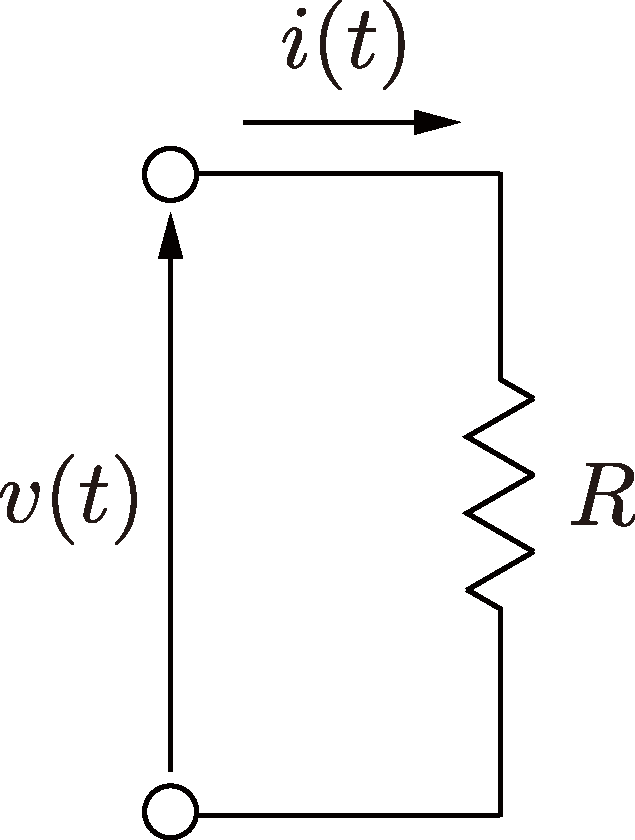
\includegraphics[width = .7\linewidth]{figs/circres2}
      \subcaption{}
      \medskip
    \end{minipage}
    \begin{minipage}{0.3\linewidth}
      \centering
      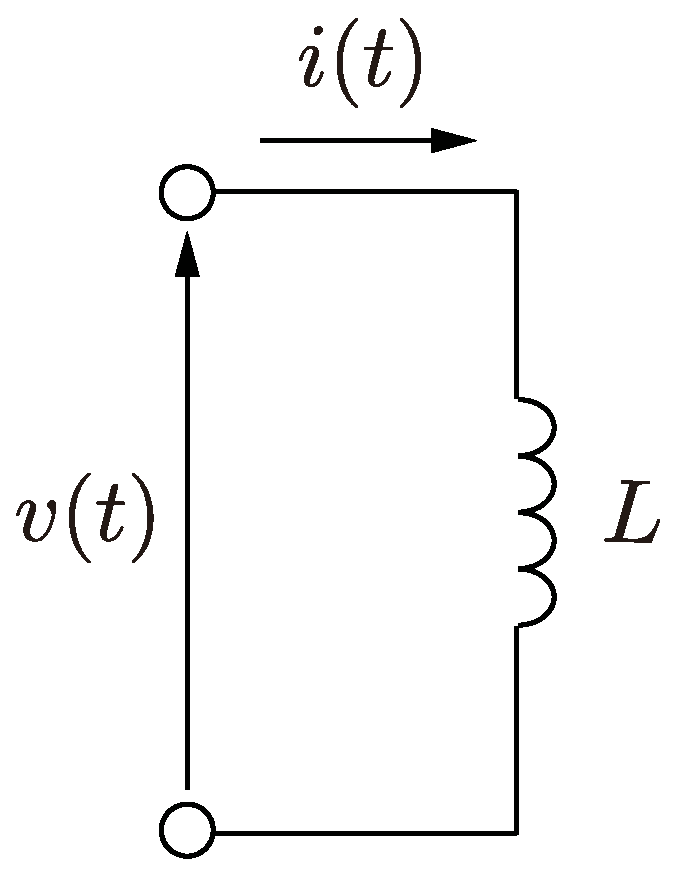
\includegraphics[width = .7\linewidth]{figs/circcoil}
      \subcaption{}
      \medskip
    \end{minipage}
    \begin{minipage}{0.3\linewidth}
      \centering
      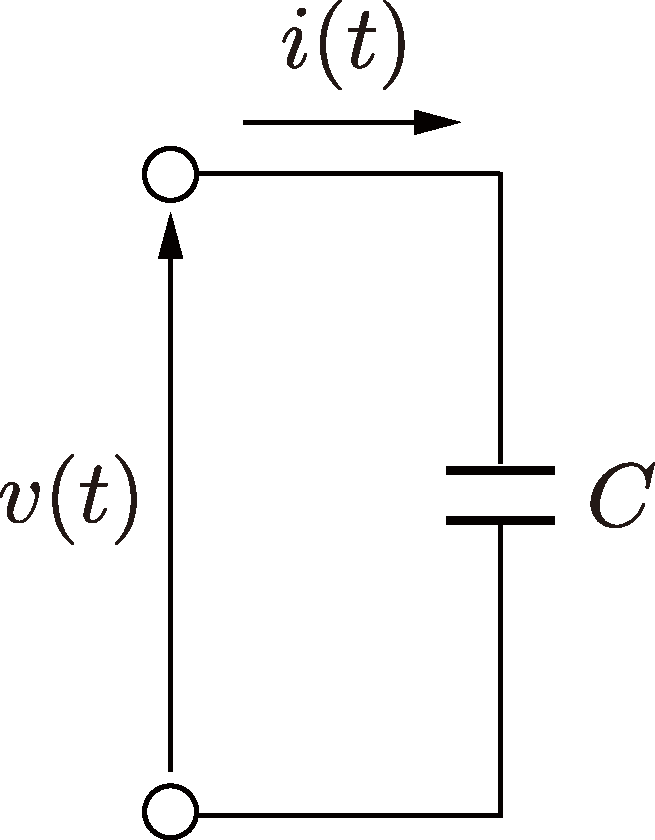
\includegraphics[width = .7\linewidth]{figs/circcond}
      \subcaption{}
      \medskip
    \end{minipage}
  }
  \medskip
  \caption{\centering Basic circuit of resistors, inductors, and
  capacitors.}
  \label{fig:basiccirc} 
  \medskip
\end{figure}

\smallskip
\begin{enumerate}[label=(\alph*)]
  \item \textbf{Resistor:} For the resistor with resistance of $R$~[$\Omega$]
  shown in \ref{fig:basiccirc}(a), the following relationship holds between the
  terminal voltage $v$~[V] and terminal current $i$~[A]:
  \begin{equation}
    v(t) = R i(t)
  \end{equation}
  where $R\geq 0$.
  \bigskip
  \item \textbf{Inductor:} For the inductor with inductance $L$~[H] shown in
  \ref{fig:basiccirc}(b), the following relationship holds between the terminal
  voltage and terminal current:
  \begin{equation}
    v(t) = L \frac{di}{dt}(t)
  \end{equation}
  where $L\geq 0$.
  \bigskip
  \item \textbf{Capacitor:} For the capacitor with capacitance $C$~[F] shown in
  \ref{fig:basiccirc}(c), the following relationship holds between the terminal
  voltage and terminal current:
  \begin{align}
    i(t) = C \frac{dv}{dt}(t)
  \end{align}
  where $C\geq 0$.
\end{enumerate}

\subsection{Instantaneous value and effective value}

\smallskip
\begin{enumerate}[label=(\alph*)]
  \item \textbf{Instantaneous value:} The instantaneous value of an AC quantity
  is an expression of this quantity in function of time $t$. For example, for a
  sinusoidal alternating voltage, its instantaneous value can be expressed by:
  \begin{equation}\label{eq:acvolt}
    v(t) = V_{\rm m} \sfsin (\omega t + \phi)
  \end{equation}
  where $V_{\rm m}$~[V] is the voltage amplitude, $\omega$~[rad/s] is the
  angular frequency, and $\phi$~[rad] is the phase. The sine wave period
  $T$~[s] is expressed as follows using $\omega$:
  \begin{equation}
    T:=\frac{2\pi}{\omega}
  \end{equation}
  Frequency $f$~[Hz] is expressed as its reciprocal $f:=\tfrac{1}{T}$. Due to
  the characteristics of the elements presented in Section \ref{sec:basicele},
  when the instantaneous value of voltage is a sine wave, the instantaneous
  value of the current also becomes a sine wave.
  \bigskip
  \item \textbf{Effective value:} The effective value of an AC quantity
  corresponds to the square root of the average of the square of the values over
  a period of time $T$. Because of this definition, the effective value is also
  called \textbf{RMS value} (root mean square value). For example, for the
  resistor in \ref{fig:basiccirc}(a), the average electric power consumed in one
  period can be calculated as follows:
  \begin{equation}\label{eq:efP}
    \frac{1}{T}
    \int_{t}^{t+T} v(\tau) i(\tau) d\tau = 
    \frac{1}{R}
    \Biggl( \underbrace{\frac{V_{\rm m}}{\sqrt{2}} }_{V_{\rm e}} \Biggr)^2
  \end{equation}
  where $V_{\rm e}$ is the \textbf{effective value} of voltage. The effective
  value of the current is defined in the same manner. Since the average electric
  power can be described simply by using the effective value of voltage and
  current, the effective value is often used to perform calculations for AC
  circuit. The effective value is also used for the phasor representation of
  voltage and current introduced below.
\end{enumerate}

\subsection{Phasor representation}\label{sec:intphas}
The AC voltage waveform of Equation \ref{eq:acvolt} can be represented in the
complex plane as in Figure \ref{fig:phasorrep}. In this case, $v(t)$ is
expressed by the following equation:
\begin{equation}\label{eq:Vcomp}
  v(t)= \imag \left[ V_{\rm m} e^{\bm{j}(\omega t + \phi)} \right]
\end{equation}

\begin{figure}[t]
  \centering
  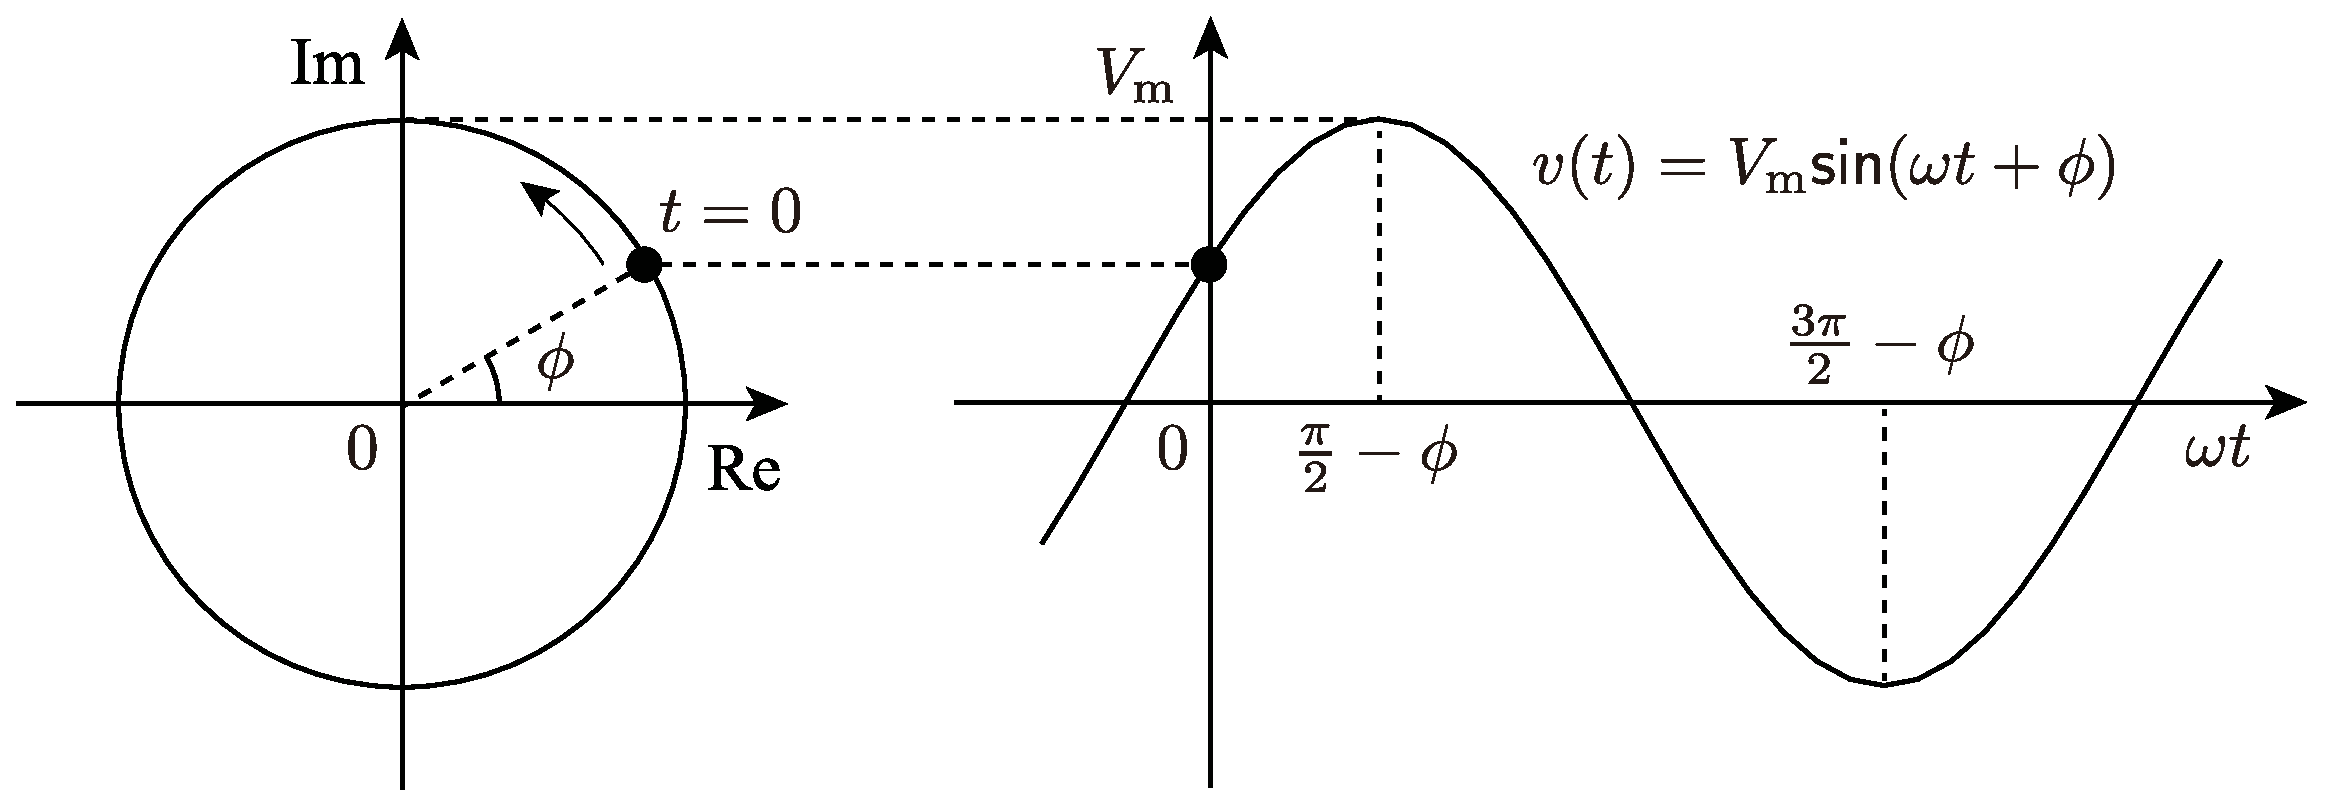
\includegraphics[width = .99\linewidth]{figs/phasorrep}
  \caption{\textbf{\red{Complex plane representation of AC voltage}}}
  \label{fig:phasorrep}
  \medskip
\end{figure}
In an electrical power system, the angular frequency $\omega$ can be considered
constant and equal to the reference angular speed. Under this assumption, the
voltage $v(t)$ of Equation \ref{eq:Vcomp} can be uniquely expressed by the phase
$\phi$, which can be derived from $\omega t$ and the amplitude $V_{\rm m}$.
Then, by using the effective value as an expression of the amplitude, we can
obtain:

\begin{align}\label{eq:Vphasor}
  \bm{V}:= V_{\rm e} e^{\bm{j}\phi}
\end{align}

This is called the \textbf{phasor representation} of voltage. When an electrical
power system is in a steady state, the phasor $\bm{V}$ is constant. In other
words, the absolute value $|\bm{V}|=V_{\rm e}$ and phase $\angle \bm{V}=\phi$
are constant. On the other hand, when an electrical power system is in a
transient state, the temporal changes of $|\bm{V}|$ and $\angle \bm{V}$ have to
be analyzed. The definition for the current phasor $\bm{I}$ is the same.

\subsection{Impedance and admittance}

The concept of impedance $\bm{Z}$~[$\Omega$] arises when expressing the
relationship between voltage and curring using the phasor representation
explained in Section \ref{sec:intphas}. It is equivalent to the resistance in DC
circuits, and corresponds to an opposition to alternating current. For the
typical circuit elements presented in Section \ref{sec:basicele}, the phasor
representations of their terminal voltage and current $\bm{V}$, $\bm{I}$ respect
the following relationship.

\begin{equation}
  \bm{V} = \bm{Z}\bm{I}
\end{equation}

The impedance of resistors, inductors and capacitors are, respectively:

\[
  \bm{Z}_{R}:=R,\qquad
  \bm{Z}_{L}:=\bm{j}\omega L,\qquad
  \bm{Z}_{C}:=\frac{1}{\bm{j}\omega C}
\]

Please note that the characteristics of components such as synchronous
generators and power converters may not be expressed using only constant
impedances.

The real part of impedance is called \textbf{resistance}and the imaginary part
is called \textbf{reactance}. As a standard symbol, $R$~[$\Omega$] is used for
resistance and $X$~[$\Omega$] is used for reactance. In other words:
\[
  \bm{Z} = R + \bm{j} X
\]
The reciprocal $\bm{Z}^{-1}$ of impedance is called \textbf{admittance}.
As a standard symbol, $\bm{Y}$~[S] is used.
In addition, the real part of admittance is called \textbf{conductance} and the imaginary part is called \textbf{susceptance}.
As a standard symbol, $G$~[S] is used for conductance and $B$~[S] is used for susceptance.
In other words:
\[
\bm{Y} = G + \bm{j} B
\]
V: volt, A: ampere, $\Omega$: ohm, H: henry, F: farad, rad: radian, s: second, Hz: hertz, and S: siemens.

\section{Admittance matrix that expresses the interaction of connected equipment}\label{sec:transadm}

\subsection{Foundation of a power grid model}


We derive the \textbf{admittance matrix} of a power grid that shows the interaction of equipment connected to an electrical power system using a basic transmission line model.
The admittance matrix is derived from Ohm’s law and Kirchhoff’s laws for each bus bar and the transmission lines that connect them.
Depending on the literature, the bus bar may also be called a \textbf{node} or \textbf{bus}.
In this book, the bus bar is shown with a thick line in the diagram of an electrical power system.
The bus bar is a conductor where the end of the transmission line has been collected. The thin line that connects the bus bar represents the transmission line.

\begin{figure}[t]
\centering
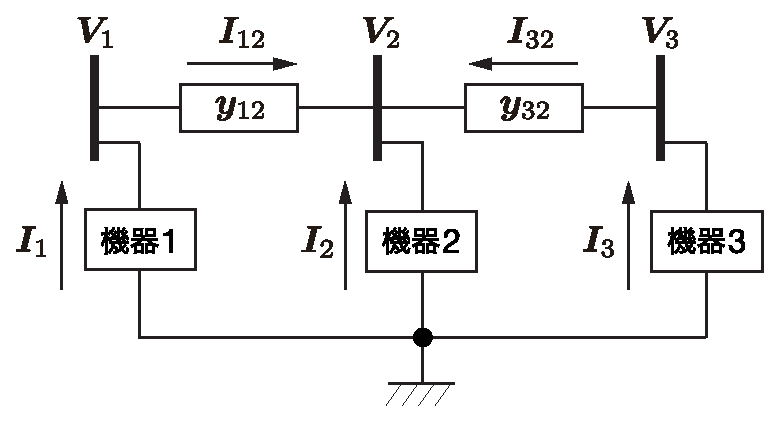
\includegraphics[width = .60\linewidth]{figs/3busex}
\medskip
\caption{\textbf{\red{Power system model consisting of three bus bars}}}
\label{fig:3busex}
\medskip
\end{figure}

\begin{example}{Admittance matrix of a power grid}\label{ex:derY}

Let us consider a simple electrical power system consisting of three bus bars
shown in \ref{fig:3busex}.  There is a piece of equipment connected to each bus
bar.  In this book, the word “equipment” refers to synchronous generators and
loads.

\footnote{ This book only assumes load from generators; however, when assuming
for solar generators, wind power generators, and batteries, these are included
in “equipment.” }

In an electrical power system model circuit such as that shown in
\ref{fig:3busex}, ground is often omitted for simplification.

Below, the voltage phasor of bus bar $i$ with ground potential is expressed as $\bm{V}_i \in \mathbb{C}$, 
and the current phase of the bus bar to bus bar $i$ that then flows from equipment $i$ is expressed as $\bm{I}_i \in \mathbb{C}$. 
These are unknown variables. The present objective is to obtain a physical equation stipulated by the power grid that holds between current phasor $(\bm{I}_1,\bm{I}_2,\bm{I}_3)$ and current phasor $(\bm{V}_1,\bm{V}_2,\bm{V}_3)$ of the bus bars. 
This corresponds to obtaining the admittance matrix of the power grid.


The admittance of a transmission line that connects bus bars $i$ and $j$ is expressed as $\bm{y}_{ij}\in \mathbb{C}$, where each one is a known constant.
In addition, phasor of the current that flows in each transmission line is expressed as $\bm{I}_{ij}\in \mathbb{C}$.
where $\bm{y}_{ij}$ and $\bm{y}_{ji}$ are equal.
In addition, the sign for $\bm{I}_{ij}$ is positive for the arbitrarily determined direction, and $\bm{I}_{ji}$ and $-\bm{I}_{ij}$ are equal.
The current phasor of this transmission line is an intermediate variable that describes the physical relationship of the current phasor and voltage phasor of the bus bars.
Specifically, as shown with the arrow in \ref{fig:3busex}, if the direction of the current phasor of each transmission line is determined, the following relationship is obtained from Ohm’s law:
\begin{align*}
\bm{I}_{12}=\bm{y}_{12}(\bm{V}_{1}-\bm{V}_{2}),\qquad
\bm{I}_{32}=\bm{y}_{32}(\bm{V}_{3}-\bm{V}_{2})
\end{align*}
It indicates that the current phasor of a transmission line is proportional to the difference in the voltage phasor between the bus bar on each end. 


According to Kirchhoff's first law (current law), since the sum of all current on each bus bar is 0, the following relationship is obtained for bus bar 1 to bus bar 3.
\begin{align*}
\bm{I}_{1}-\bm{I}_{12}=0,\qquad
\bm{I}_{2}+\bm{I}_{12}+\bm{I}_{32}=0,\qquad
\bm{I}_{3}-\bm{I}_{32}=0
\end{align*}
If an intermediate variable, $\bm{I}_{ij}$, is removed from this Equation, the following is obtained as the vectorized Ohm's law of the bus bar, which holds between the voltage phasor and current phasor:

\begin{align}\label{eq:exY}
\mat{
\bm{I}_1\\
\bm{I}_2\\
\bm{I}_3\\
}
=
\mat{
\bm{y}_{12} & -\bm{y}_{12} & 0\\
-\bm{y}_{12} & \bm{y}_{12}+\bm{y}_{32} & -\bm{y}_{32}\\
0 & -\bm{y}_{32} & \bm{y}_{32}
}
\mat{
\bm{V}_1\\
\bm{V}_2\\
\bm{V}_3\\
}
\end{align}
The complex matrix obtained in this manner is the admittance matrix of the power grid.
Since each transmission line is usually expressed as an equivalent circuit of resistance and inductance, the real part (conductance) of admittance $\bm{y}_{ij}$ of the transmission line is non-negative, and the imaginary part (susceptance) is non-positive.
Specifically, the imaginary part is usually negative (non-zero).
\end{example}

Below, we consider an electrical power system connected with $N$ bus bars.
\begin{align}\label{eq:ohmY}
\mat{
  \bm{I}_1\\
  \vdots\\
  \bm{I}_N
}
 =
\underbrace{
\mat{
  \bm{Y}_{11} & \cdots & \bm{Y}_{1N}\\
  \vdots & \ddots & \vdots\\
  \bm{Y}_{N1} & \cdots & \bm{Y}_{NN}
}
}_{\bm{Y}}
\mat{
  \bm{V}_1\\
  \vdots\\
  \bm{V}_N
}
\end{align}
At this time, the admittance matrix $\bm{Y} \in \mathbb{C}^{N \times N}$ of the power grid gives the following relationship to the current phasor $(\bm{I}_1,\ldots,\bm{I}_N)$ and voltage phasor $(\bm{V}_1,\ldots,\bm{V}_N)$ of the bus bars.
Equation \ref{eq:ohmY} is a “mathematical model of the power grid” that expresses interactions related to input and output for equipment connected to the bus bars. 
Specifically, if we consider voltage phasor $\bm{V}_i$ as an output from equipment $i$ to the electrical power system, and current phasor $\bm{I}_i$ as an input from the electrical power system to equipment $i$, the input to equipment $i$ is expressed as a linear combination of output from other equipment:
 \begin{align*}
 \bm{I}_i = \bm{Y}_{i1}  \bm{V}_1 + \cdots +\bm{Y}_{iN}  \bm{V}_N
 \end{align*}
The real part and imaginary parts of the admittance matrix are called the \textbf{conductance matrix} and \textbf{susceptance matrix}, respectively.

The simultaneous equations of Equation \ref{eq:ohmY} provide “a part” of an equation related to the current phasor and voltage phasor of the bus bars, and unknown variables $(\bm{I}_1,\ldots,\bm{I}_N)$ and $(\bm{V}_1,\ldots,\bm{V}_N)$ cannot be uniquely determined.
To uniquely determine the steady and transient behavior of all current phasors and voltage phasors, the relationship of localized $\bm{I}_i$ and $\bm{V}_i$ that expresses the characteristics of each equipment must be separately determined.
This localized relationship is “the mathematical model that expresses the input-output relationship of each device.”
Specific mathematical models of synchronous generators and loads will be described in detail in Section \ref{sec:genmod} and beyond.

Determining a model for the power grid model of Equation \ref{eq:ohmY} and a model of the equipment group discussed below is equivalent to determining the mathematical model for the entire electrical power system.
The structure of the entire electrical power system is shown in \ref{fig:overviewpwmod}.
The block of “equipment $i$” is the mathematical model that expresses the input-output relationship for each device, while the block of “algebraic equation of power grid” expresses the vectorized Ohm’s law of Equation \ref{eq:ohmY}.


\begin{figure}[t]
\centering
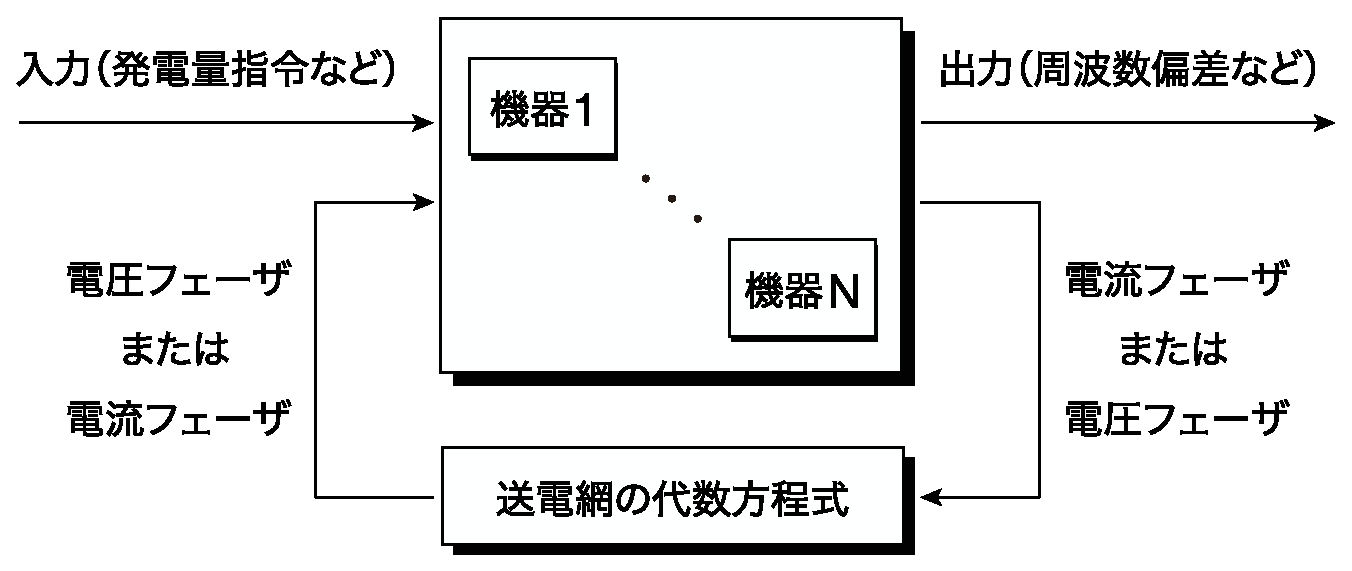
\includegraphics[width = .80\linewidth]{figs/overview}
\medskip
\caption{
\textbf{\red{Schematic diagram of the power system model}}
}
\label{fig:overviewpwmod}
\medskip
\end{figure}


In Equation \ref{eq:ohmY}, current phasor $\bm{I}_i$ can be considered as an output from equipment $i$ to the electrical power system, and current phasor $\bm{V}_i$ as an input from the electrical power system to equipment $i$.
In this case, as well, with an appropriate impedance matrix $\bm{Z}\in \mathbb{C}^{N\times N}$, it can be formally expressed as follows:
 \begin{align}\label{eq:ohmZ}
 \mat{
  \bm{V}_1\\
  \vdots\\
  \bm{V}_N
}
=
\underbrace{
\mat{
  \bm{Z}_{11} & \cdots & \bm{Z}_{1N}\\
  \vdots & \ddots & \vdots\\
  \bm{Z}_{N1} & \cdots & \bm{Z}_{NN}
}
}_{\bm{Z}}
\mat{
  \bm{I}_1\\
  \vdots\\
  \bm{I}_N
}
\end{align}
However, if the admittance matrix $\bm{Y}$ in Equation \ref{eq:ohmY} is nonsingular, $\bm{Z}=\bm{Y}^{-1}$, 
but $\bm{Y}$ is not always nonsingular. For example, since the admittance matrix of Equation \ref{eq:exY} is not nonsingular, 
the following holds:
\[
\bm{V}_1=\bm{V}_2=\bm{V}_3
\qquad  \Longrightarrow \qquad 
\bm{I}_1=\bm{I}_2=\bm{I}_3=0
\]
The irregularity of this admittance matrix indicates that “when all current phasors of each bus bar are 0, all voltage phasors are the same; however, the value cannot be uniquely determined.”
However, within the scope of normal analysis, there is rarely any need to pay attention to whether the admittance matrix is nonsingular.

\begin{figure}[t]
\centering
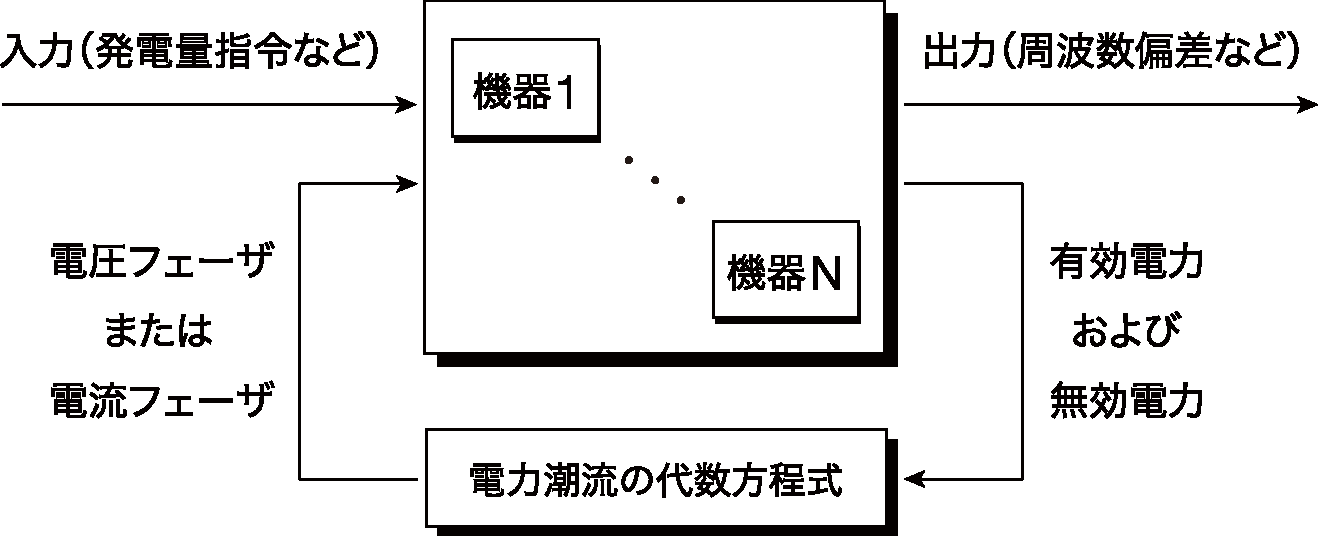
\includegraphics[width = .80\linewidth]{figs/overviewPQ}
\medskip
\caption{\textbf{Schematic diagram of power system model}}
\label{fig:overviewpwmodPQ}
\medskip
\end{figure}

In addition, active power $P_i \in \mathbb{R}$ and reactive power $Q_i \in \mathbb{R}$ provided from equipment $i$ to bus bar $i$ are defined by: 
\[
P_i := \real \left[ \bm{V}_i \overline{\bm{{I}} }_i \right], \qquad
Q_i := \imag \left[ \bm{V}_i \overline{\bm{{I}} }_i \right]
\]
In other words, the following relationship holds between active power, reactive power, bus bar voltage phasor, and bus bar current phasor.

\begin{align}\label{eq:defPQVIi}
P_i+\bm{j}Q_i = \bm{V}_i \overline{\bm{{I}} }_i
\end{align}
With that, by equivalently expressing the power grid model of Equation \ref{eq:ohmY} as follows:
\begin{align}\label{eq:ohmpf}
\simode{
P_i &= \sum_{j=1}^{N}
\real \left[ \overline{\bm{Y}}_{ij} \bm{V}_i \overline{\bm{V}}_j 
\right] \\
Q_i &= \sum_{j=1}^{N}
\imag \left[
\overline{\bm{Y}}_{ij} \bm{V}_i \overline{\bm{V}}_j 
\right]
}
\qquad
i \in \{1,\ldots, N\}
\end{align}

An electrical power system model that uses active power and reactive power provided to the bus bar as an output of equipment is obtained (\ref{fig:overviewpwmodPQ}).
Equation \ref{eq:ohmpf} is a simultaneous equation that expresses the electric power flow in each bus bar.
\ref{fig:overviewpwmod} and \ref{fig:overviewpwmodPQ} are equal electrical power system models, but two models can be used according to the analysis purpose.

\subsection{Power grid model that considers capacitance to ground}\label{sec:transmodc}

In a short transmission lines, the model from the example \ref{ex:derY} is used; however, in mid-distance transmission lines that exceed 50 km, the capacitance to ground (capacitance component) created between the transmission line and the ground cannot be ignored. 
As a transmission line model that considers the capacitance to ground, the $\pi$t-ype equivalent circuit shown in \ref{fig:lines} is often used.
However, in \ref{fig:lines}, a transmission line that uses bus bar 1 and bus bar 2 as end points is shown, where $\omega_0$ shows a system frequency and $c_{12}$ shows capacitance that expresses the capacitance to ground.
The admittance matrix of the power grid, when this transmission line model is used, is obtained as follows: 

\begin{figure}[t]
\centering
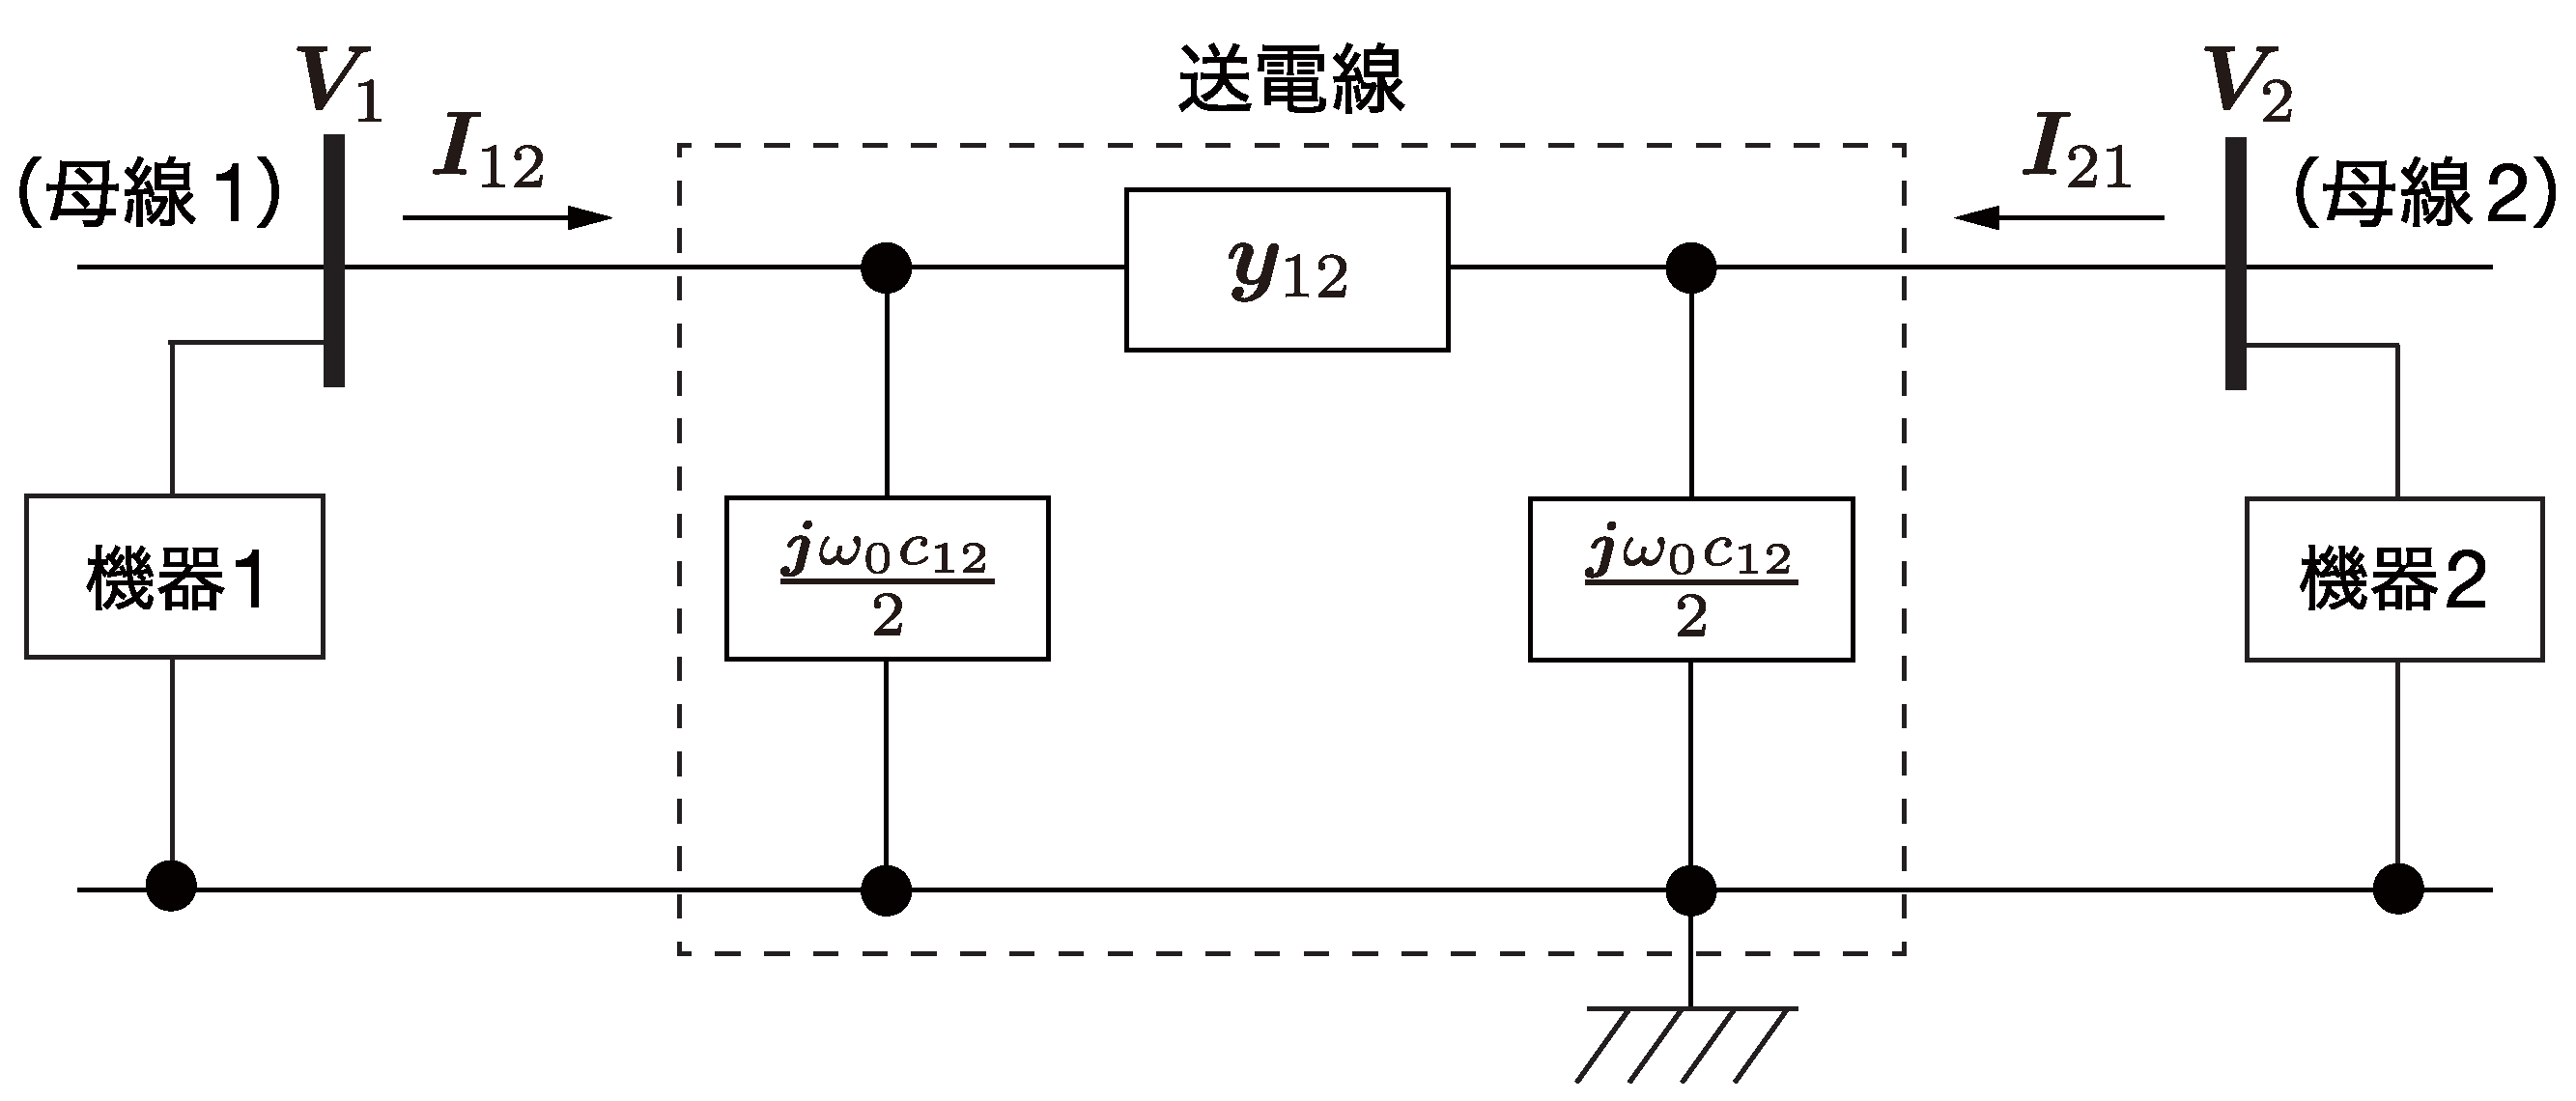
\includegraphics[width = .85\linewidth]{figs/line_pix3}
\medskip
\caption{\textbf{$\pi$-type circuit model of a transmission line with ground-to-ground capacitance}\\
\centering(Transmission lines with end points at bus bar 1 and bus bar 2)}
\label{fig:lines} 
\medskip
\end{figure}


%\begin{figure}[t]
%  \centering
%  {
%  \begin{minipage}{0.49\linewidth}
%    \centering
%    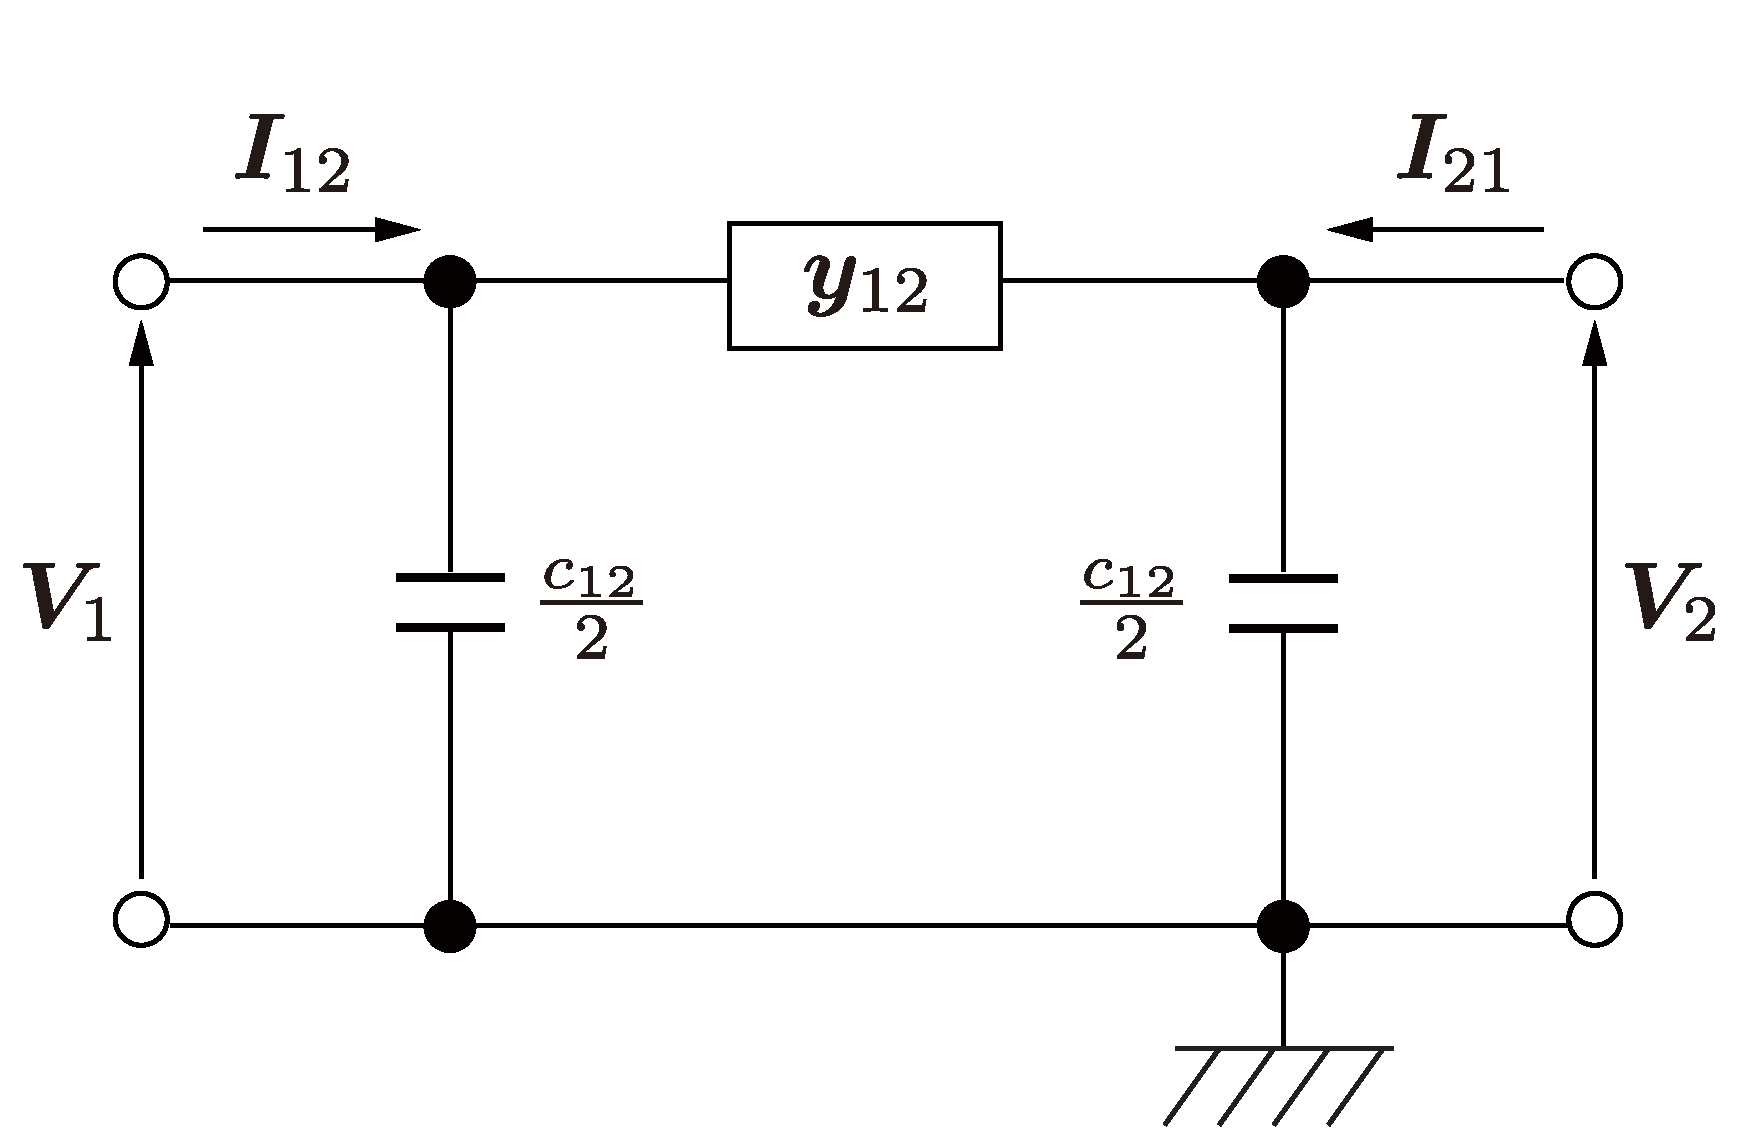
\includegraphics[width = .99\linewidth]{figs/line_pix}
%%    \medskip
%    \subcaption{$\pi$型等価回路}
%%    \label{fig:line_pi} 
%  \end{minipage}
%  \begin{minipage}{0.49\linewidth}
%    \centering
%    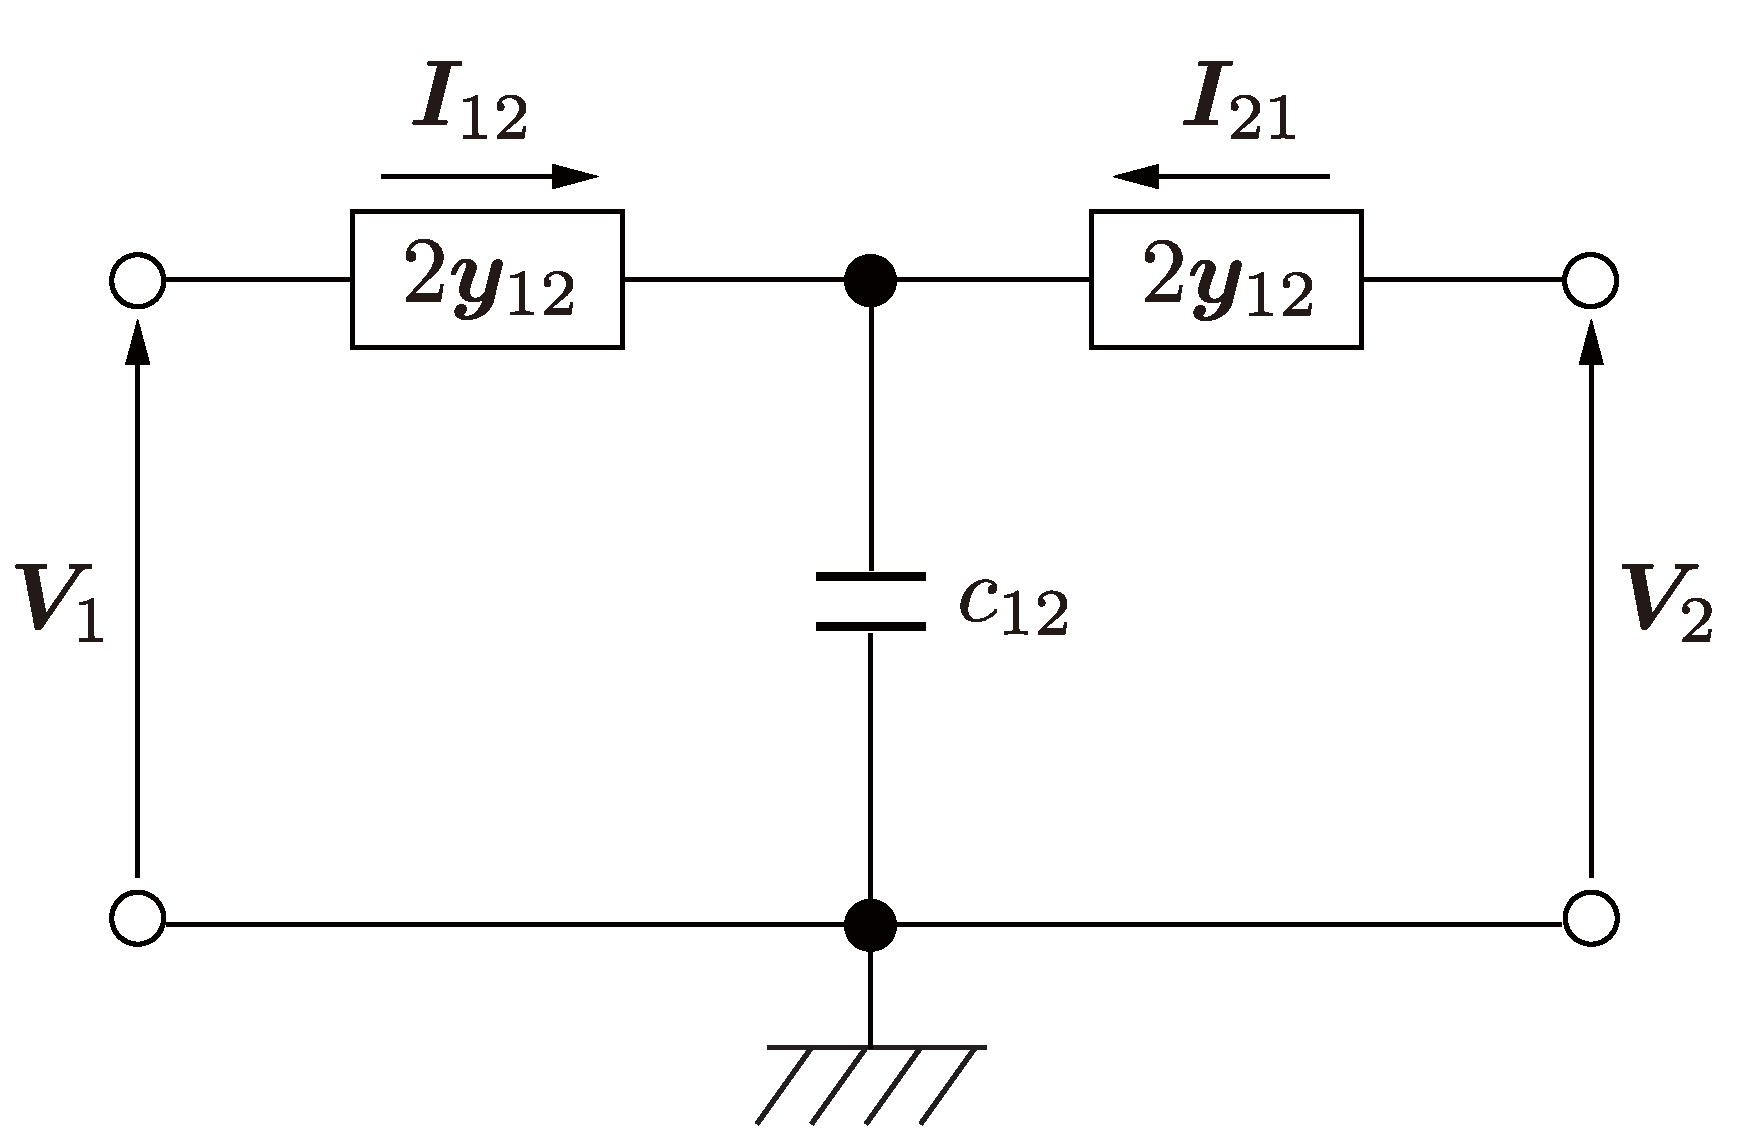
\includegraphics[width = .99\linewidth]{figs/line_Tx}
%%    \medskip
%    \subcaption{T型等価回路}
%%    \label{fig:lines} 
%  \end{minipage}
%  }
%\medskip
%\caption{\textbf{対地静電容量を考慮した送電線のモデル}}
%\label{fig:lines} 
%\medskip
%\end{figure}


%\begin{figure}[t]
%  \centering
%  {
%    \centering
%    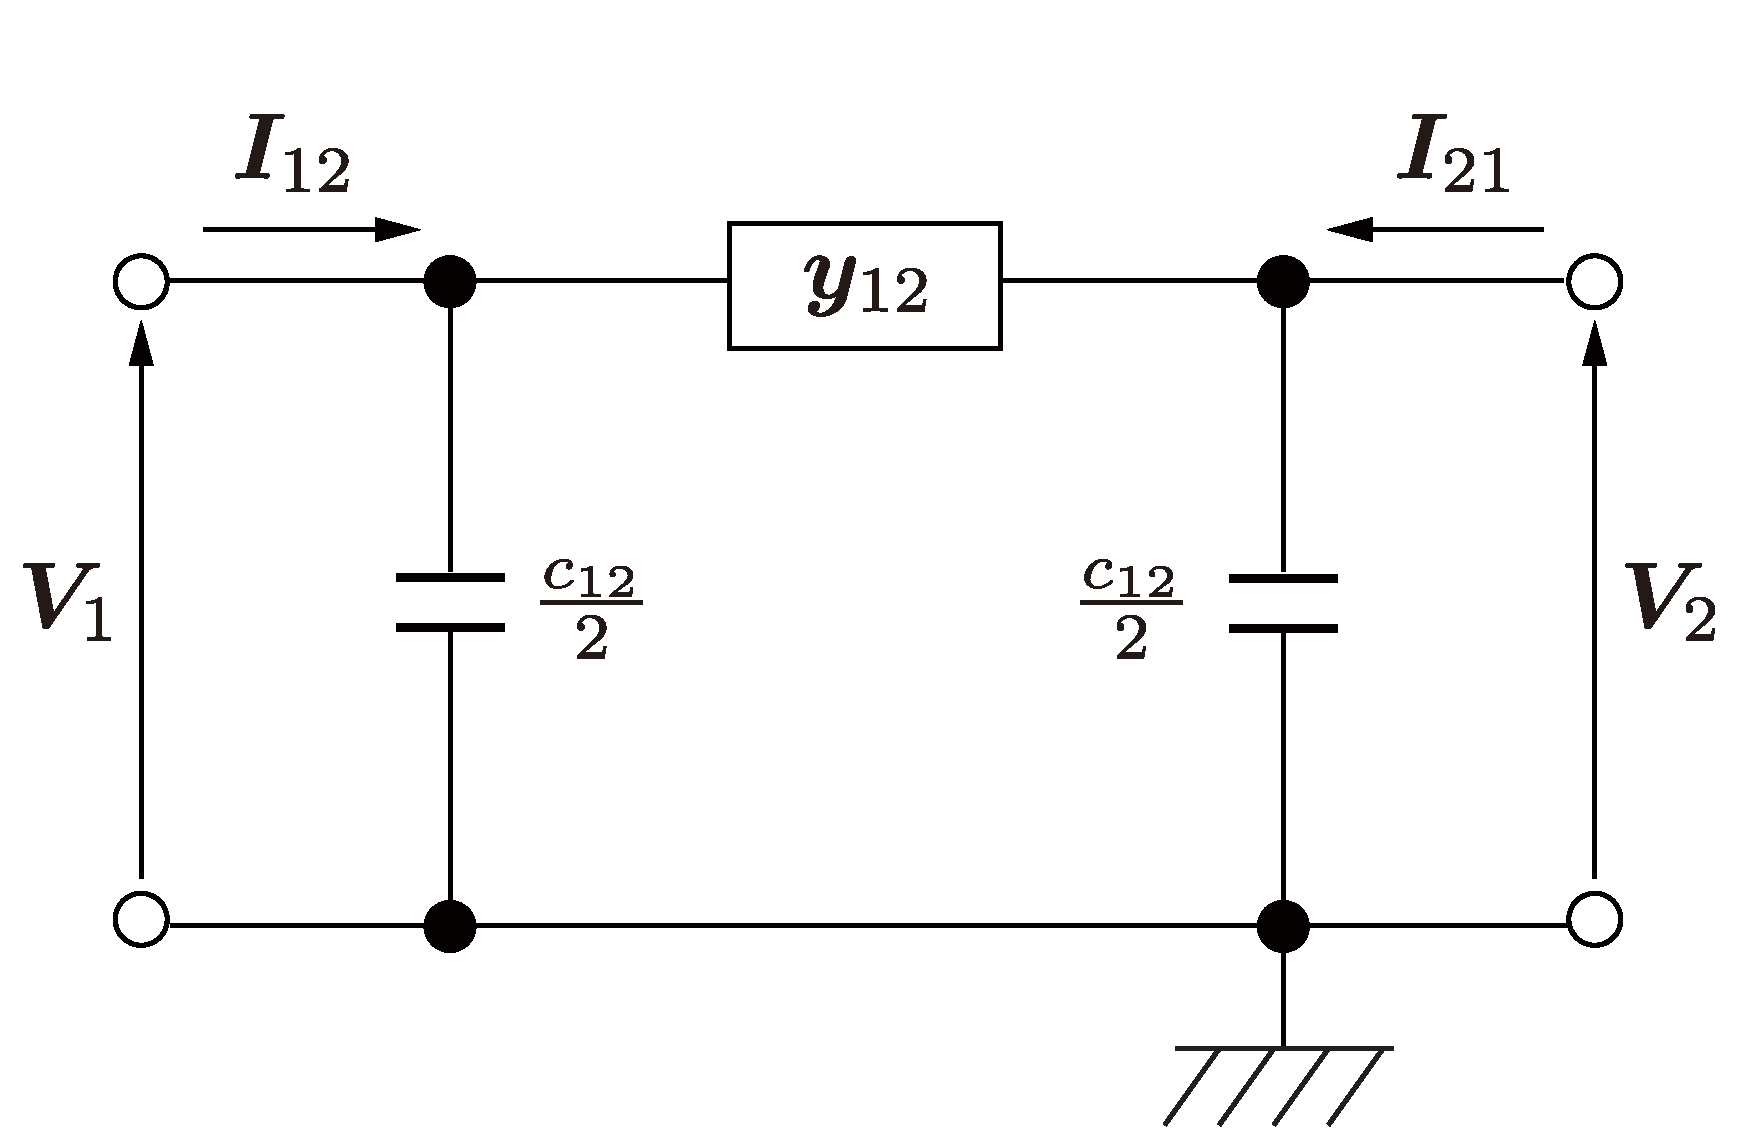
\includegraphics[width = .55\linewidth]{figs/line_pix}
%    \subcaption{$\pi$型等価回路}
%    \label{fig:line_pi} 
%    \centering
%    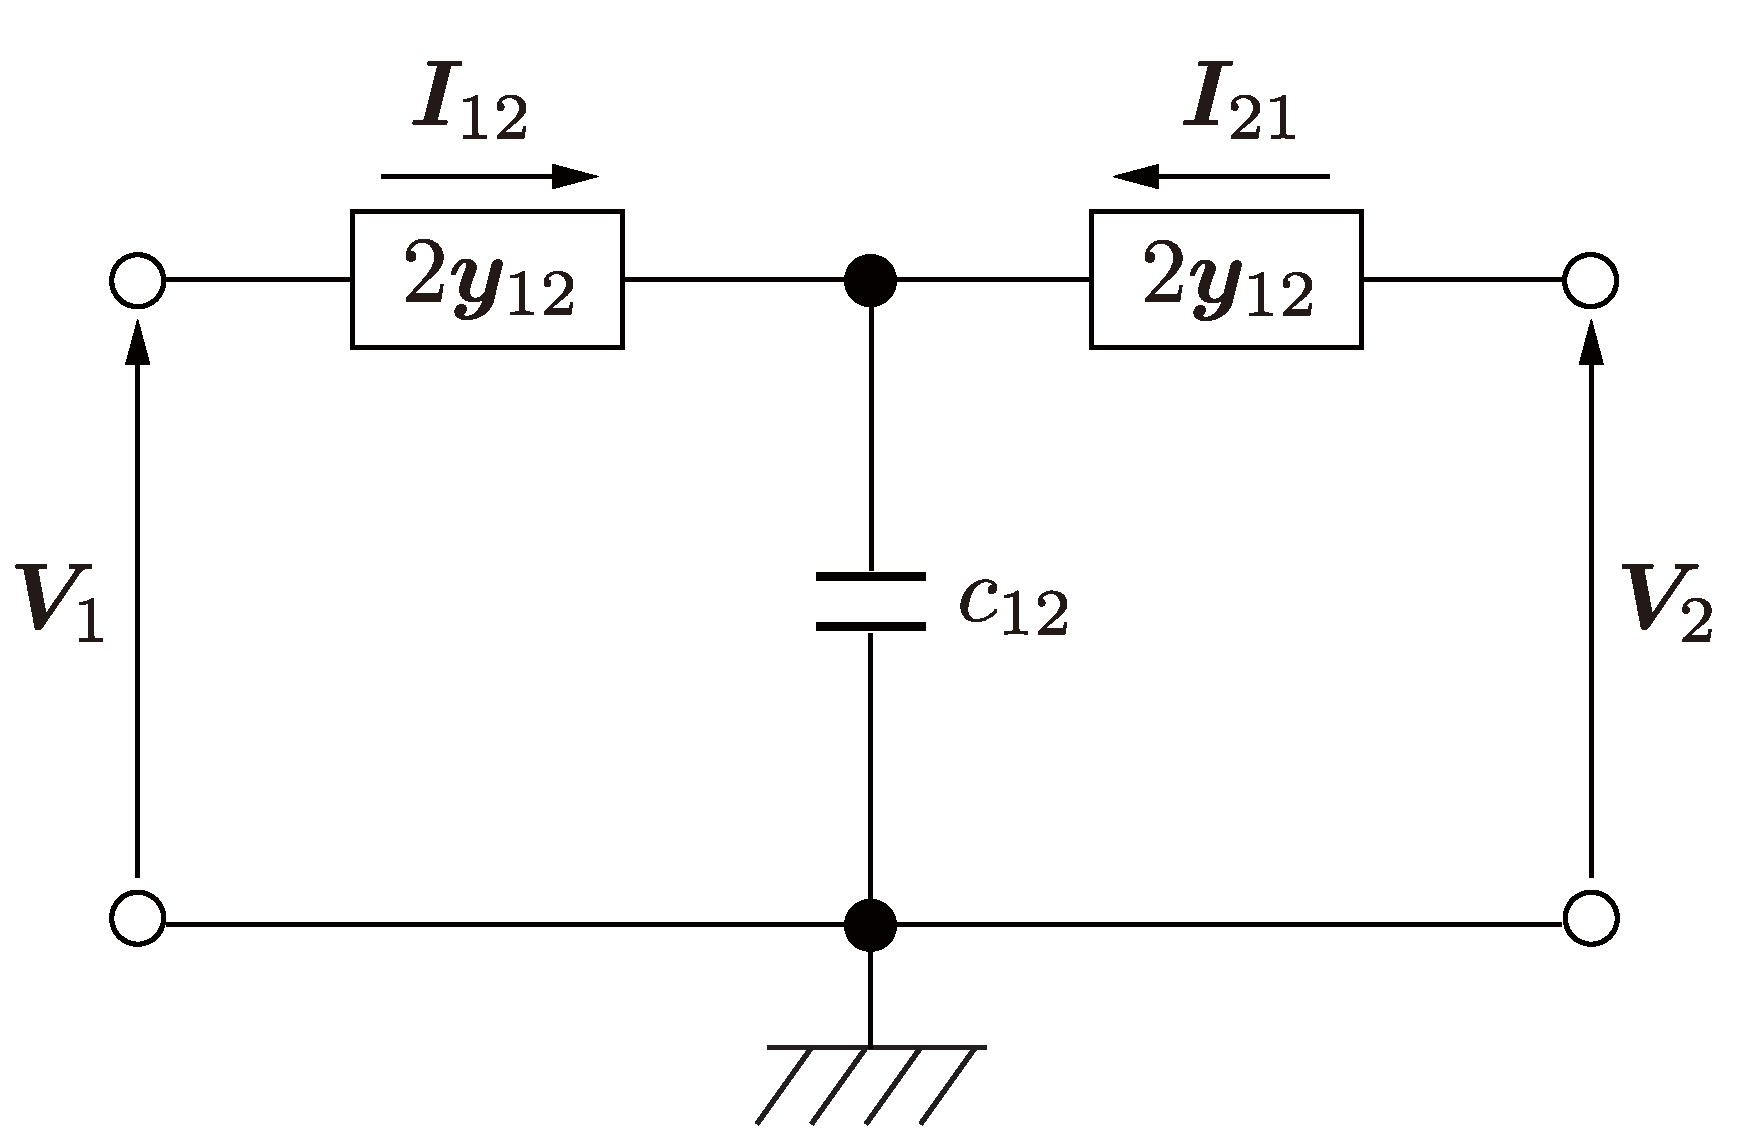
\includegraphics[width = .55\linewidth]{figs/line_Tx}
%    \subcaption{T型等価回路}
%  }
%  \medskip
%   \caption{\textbf{対地静電容量を考慮した送電線のモデル}}
%   \label{fig:lines}
%\medskip
%\end{figure}


\begin{example}{Admittance matrix for the transmission line in a $\pi$-type circuit}\label{ex:pitypeY}

  In an electrical power system similar to the example \ref{ex:derY}, derive the admittance matrix when the transmission line is expressed with a $\pi$-type equivalent circuit. 
  First, consider the relationship of current phasors $\bm I_{12}$, $\bm I_{21}$, flowing from the bus bar, and voltage phasors $\bm V_1$, $\bm V_2$ of the bus bar on a line that uses bus bar 1 and bus bar 2 of \ref{fig:lines} as end points. 
  At this time, please note that, unlike the case of example \ref{ex:derY}, $\bm I_{21}$ is different from $-\bm I_{12}$. If the current flowing through the line with the admittance of $\Ysa$ from left to right is expressed as $\Is$, the following holds based on Kirchhoff's laws:
  \begin{align*}
      \bm I_{12} = \frac{\bm{j} \omega_0 \bca}{2} \bm V_1 + \Is ,\qquad
      \frac{\bm{j} \omega_0 \bca}{2} \bm V_2 = \bm I_{21} + \Is
  \end{align*}
  And with Ohm’s law, the following holds: 
  \begin{align*} \Is = \Ysa(\bm V_1-\bm V_2)\end{align*}
  By removing $\Is$ and reorganizing, we obtain:
  \begin{align*}
    \mat{
      \bm I_{12} \\ \bm I_{21}
    } = \mat{
      \Ysa +  \tfrac{\bm{j} \omega_0 \bca}{2} & -\Ysa \\
      -\Ysa & \Ysa+  \tfrac{\bm{j} \omega_0 \bca}{2}
    }
    \mat{
      \bm V_1\\\bm V_2
    }
  \end{align*}
  The following is true for the transmission line that uses bus bar 2 and bus bar 3 as end points:
  \begin{align*}
    \mat{
      \bm I_{32} \\ \bm I_{23}
    } = \mat{
      \Ysb + \tfrac{\bm{j} \omega_0 \bcb}{2} & -\Ysb \\
      -\Ysb & \Ysb+ \tfrac{\bm{j} \omega_0 \bcb}{2}
    }
    \mat{
      \bm V_3 \\ \bm V_2
    }
  \end{align*}
  Therefore, by using:
  \begin{align*}
    \bm{I}_{1}-\bm{I}_{12}=0,\qquad
    \bm{I}_{2}-\bm{I}_{21}-\bm{I}_{23}=0,\qquad
    \bm{I}_{3}-\bm{I}_{32}=0
    \end{align*}
  The admittance matrix of the power grid can be obtained as: 
  \begin{align*}%\label{eq:Ypitype}
    \mat{
    \bm{I}_1\\
    \bm{I}_2\\
    \bm{I}_3\\
    }
    =
    \mat{
    \bm{y}_{12} + \tfrac{\bm{j} \omega_0 \bca}{2} & -\bm{y}_{12} & 0\\
    -\bm{y}_{12} & \hspace{-3mm} \bm{y}_{12}+\bm{y}_{32} + \tfrac{\bm{j} \omega_0 (\bca+\bcb)}{2} & -\bm{y}_{32}\\
    0 & -\bm{y}_{32} & \hspace{-3mm} \bm{y}_{32}+ \tfrac{\bm{j} \omega_0 \bcb}{2}
    }
    \mat{
    \bm{V}_1\\
    \bm{V}_2\\
    \bm{V}_3\\
    }
  \end{align*}
 This is consistent with Equation \ref{eq:exY} when $\bca$ and $\bcb$ are zero.
\end{example}

\subsection{Mathematical properties of the admittance matrix}\label{sec:admathp}

In this book, it is assumed that the power grids are connected; in other words, there is at least one route connecting two arbitrarily chosen bus bars. For unconnected power grids, the connected part(s) can be independently discussed.
In \ref{fig:congraphab}, the node (circle) corresponds to the bus bars and the edge (black line) corresponds to the transmission lines.

In the power grid model of example \ref{ex:derY} where capacitance to ground is ignored, the admittance matrix is specially expressed as $\bm{Y}_0 \in \mathbb{C}^{N\times N}$. 
The real and imaginary parts of $\bm{Y}_0$; in other words, conductance matrix and susceptance matrix, are expressed as:
\[
G_0:=\real [\bm{Y}_0] ,\qquad
B_0:=\imag [\bm{Y}_0]
\]

These matrices have the following properties.
First, the following is true for vectors where all elements are one $\mathds{1}\in \mathbb{R}^N$:
\begin{subequations}\label{eq:Y0prop}
\begin{align}\label{eq:Y0ker}
\bm{Y}_0 \mathds{1} =0
\qquad
\Longleftrightarrow
\qquad
G_0\mathds{1} =0,\qquad
B_0\mathds{1} =0
\end{align}
This means that the sum of elements in all row vectors is zero for the conductance and susceptance matrices.
Furthermore, since conductance is non-negative and susceptance is negative in each transmission line, the conductance matrix is positive semi-definite and the susceptance matrix is negative semi-definite; in other words: 
\begin{align}\label{eq:Y0}
G_0 =G_0^{\sfT} \succeq 0,\qquad
B_0 = B_0^{\sfT} \preceq 0
\end{align}
Specifically, based on the fact that the connectivity of the power grid and the susceptance of the transmission line are non-zero, the multiplicity of the zero eigenvalue of $B_0$ is derived to be 1.
This can also be expressed as:
\begin{align}\label{eq:Y0eig}
\sfker B_0 = \sfspan \{ \mathds{1} \}
\end{align}
In graph theory terms, $-B_0$ is \textbf{graph Laplacian} of a strongly connected weighted undirected graph.
The multiplicity of the zero eigenvalue in graph Laplacian being 1 is a requirement for the corresponding undirected graph to be strongly connected \cite{mesbahi2010graph}.

%\footnote{
%%\blue{ \footnotesize(あとで脚注に変更)
%グラフ理論の用語では, $-B_0$は強連結な重み付き無向グラフの\textbf{グラフラプラシアン}(graph Laplacian)である。
%グラフラプラシアンの零固有値の重複度が1であることは, 対応する無向グラフが強連結であるための必要十分条件である\cite{mesbahi2010graph}。
%}
%。
\end{subequations}



\begin{figure}[t]
  \centering
  {
  \begin{minipage}{0.42\linewidth}
    \centering
    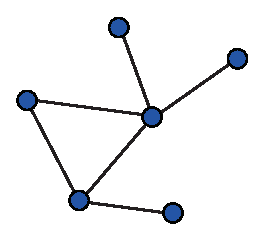
\includegraphics[width = .6\linewidth]{figs/congraph}
    \medskip
    \subcaption{Connected graph}
    \label{fig:congraph} 
  \end{minipage}
  \begin{minipage}{0.42\linewidth}
    \centering
    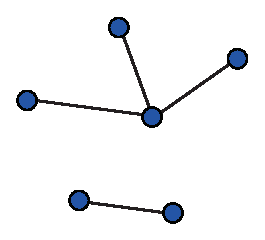
\includegraphics[width = .6\linewidth]{figs/notcongraph}
    \medskip
    \subcaption{Unconnected graphs}
    \label{fig:notcongraph} 
  \end{minipage}
  }
\medskip
\caption{\textbf{Connected and disconnected graphs}
\\
\centering(Connected graph and unconnected graph)}
\label{fig:congraphab} 
\medskip
\end{figure}

Furthermore, in the power grid model expressed with the $\pi$-type equivalent circuit in the example \ref{ex:pitypeY}, a non-negative value is added to the diagonal element of the susceptance matrix $B_0$.
In other words, the admittance matrix for the power grid model in examples \ref{ex:derY} and \ref{ex:pitypeY} can usually be expressed as:
\begin{align}\label{eq:Ypig}
\bm{Y} = G_0 + \bm{j} \left( B_0 + \sfdiag( \Cgi )_{i \in \{1,\ldots,N\}} \right)
\end{align}
where $ \Cgi $ is a non-negative constant equivalent to capacitance to ground, and the conductance matrix $G_0$ and the susceptance matrix $B_0$ satisfy Equation (\ref{eq:Y0prop}).

\section{Mathematical model for synchronous generators}\label{sec:genmod}

\subsection{Division of generator models based on the level of detail}

In electrical power system engineering, different synchronous generator models with different levels of detail, such as consideration to field winding and damper winding, have been used to analyze the stability of an electrical power system [4, 5, 8, 9].
Here, we present four types of models.

\smallskip
\subsubsection{Park model}

A model with a high level of detail that considers the change in magnetic flux in the stator, field winding, and damper winding is called a \textbf{Park model} or, at times, called a \textbf{detailed model}.
It consists of a two-dimensional linear differential equation (oscillation equation) that expresses the mechanical dynamic characteristics of the rotor of a generator, or a five- to seven-dimensional nonlinear differential equation that expresses the magnetic flux changes in the stator, field winding, and damper winding.
The dimension of the latter differential equation that expresses changes in magnetic flux varies based on the number of windings to consider and the setting of variables.
The active power and reactive power, which represent the electrical output of a generator, are nonlinear functions for the internal state of the generator.
The models used in Japanese works consider a type of damper winding on the d-axis and two types of damper windings on the q-axis in addition to field winding on the d-axis [8]. 
When there is only one type of damper winding on the q-axis, if the constant is set appropriately, there are no issues in terms of practical use.

\smallskip
\subsubsection{Two-axis model}

In terms of the dynamic characteristics of magnetic flux change in stators and damper winding, a model that approximates the differential equation to the algebraic equation, assuming that their time constant is sufficiently small, is called the \textbf{two-axis model} [9. Section 5.4].
It consists of a two-dimensional oscillation equation and a two-dimensional nonlinear differential equation that expresses the magnetic flux change in field winding and damper winding.
Generally, the dynamic characteristics of magnetic flux change in the stator and damper winding are sufficiently faster than other dynamic characteristics; thus, the behavior of the Park model is generally well approximated.

\smallskip
\subsubsection{One-axis model}

In contrast to the two-axis model, a model that is obtained by assuming that the time constant of the magnetic flux change in damper winding is 
sufficiently small is called the \textbf{one-axis model}[10-12], which is at times called a \textbf{transient model}.
It consists of a two-dimensional oscillation equation and a one-dimensional nonlinear differential equation that expresses the magnetic flux change in the field winding.
In this book, we use a one-axis model to perform analysis.
The process of deriving a one-axis model from the Park model is explained in \cite[Section 5]{sauer2017power} and \cite[Section 4.15]{anderson2008power}.

\smallskip
\subsubsection{Classical model }

A model that ignores magnetic flux changes in the field winding and damper winding is called a \textbf{classical model}.
In Japanese, it is also called a \textbf{constant back voltage model} \cite{kato2017electric}. 
The generator itself consists of a linear two-dimensional oscillation equation, but the fact that the active power and reactive power are nonlinear functions of the internal state of the generator is the same.
It is widely used today as a model that analyzes the oscillatory and synchronization phenomena of electrical power systems [10-14].

\subsection{Mathematical expression of one-axis model}\label{sec:genfund}

\smallskip
\subsubsection{Relational expression of current and voltage where the internal state of a generator is the intermediate variable}

If the internal voltage of a generator $i$ connected to a bus bar $i$ is $E_i$, and the rotor argument relative to a coordinate system that rotates with a system frequency $\omega_0$ is $\delta_i$, the following relationship holds for the voltage phasor $\bm{V}_i$ of bus bar $i$ and current phasor $\bm{I}_i$ flowing from the generator to the bus bar $i$:
\begin{subequations}\label{eq:phVIs}
\begin{align}\label{eq:phVI}
\bm{I}_i  = \frac{1}{ \bm{j} \Xti } \left(E_i e^{\bm{j} \delta_i} - \bm{V}_i \right)
\end{align}
where $\Xti$ is the transient reactance of the generator.
The schematic is shown in \ref{fig:generatorbus}.
The ground is omitted from the Figure.

\begin{figure}[t]
\centering
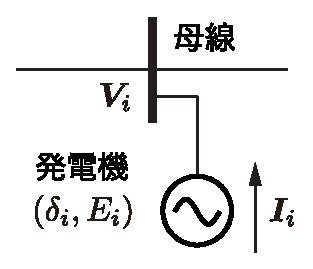
\includegraphics[width = .25\linewidth]{figs/generatorbus}
\medskip
\caption{\textbf{Generator connected to bus bar}}
\label{fig:generatorbus}
\medskip
\end{figure}


$\delta_i$ and $E_i$ in Equation \ref{eq:phVI} are intermediate variables that express the internal state of the generator $i$, which give a dynamic relationship between $\bm{I}_i$ and $\bm{V}_i$.
In other words, from the perspective of control systems engineering, Equation \ref{eq:phVI} uses $\delta_i$ and $E_i$ as the internal state, and can be interpreted as an “output equation” of a generator $i$, when $\bm{I}_i$ is the output from the generator to the electrical power system and $\bm{V}_i$ is the input from the electrical power system to the generator.
Equally, it can be considered that $\bm{V}_i$ is the output and $\bm{I}_i$ is the input.
Details will be discussed later.
By multiplying both sides of the Equation \ref{eq:phVI} with $e^{- \bm{j}\delta}$ and considering the equation for the real part and the imaginary part separately, we can see that Equation \ref{eq:phVI} is equivalent to:
\begin{align}\label{eq:phVIsincos}
\spliteq{
|\bm{V}_i| \sfsin (\delta_i -\angle \bm{V}_i)  &= 
\Xti |\bm{I}_i| \sfcos (\delta_i -\angle \bm{I}_i), \\
|\bm{V}_i| \sfcos (\delta_i -\angle \bm{V}_i)  &= 
E_i - \Xti |\bm{I}_i| \sfsin (\delta_i -\angle \bm{I}_i)
}
\end{align}
\end{subequations}



Active power $P_i$ provided from the generator $i$ to the bus bar $i$ and can be expressed as:
\begin{align*}
\spliteq{
P_i&=\real \left[ \bm{V}_i \overline{ \bm{I} }_i \right]  
\\
&= 
\real \left[ |\bm{V}_i|e^{ -\bm{j} (\delta_i -\angle \bm{V}_i )} \overline{|\bm{I}_i | e^{ -\bm{j} ( \delta_i - \angle \bm{I}_i)} } \right]
\\
&=
|\bm{V}_i| |\bm{I}_i| 
\sfcos(\delta_i -\angle \bm{V}_i) \sfcos(\delta_i -\angle \bm{I}_i) \\
 & \hspace{10em} +|\bm{V}_i| |\bm{I}_i|
\sfsin(\delta_i -\angle \bm{V}_i) \sfsin(\delta_i -\angle \bm{I}_i)
}
\end{align*}
Similarly, reactive power $Q_i$ can be expressed as:
\begin{align*}
\spliteq{
Q_i&=\imag \left[ \bm{V}_i \overline{ \bm{I} }_i \right] \\
&=
|\bm{V}_i| |\bm{I}_i | \sfcos(\delta_i -\angle \bm{V}_i ) \sfsin(\delta_i -\angle \bm{I}_i) \\
 & \hspace{10em} - |\bm{V}_i| |\bm{I}_i| \sfsin(\delta_i -\angle \bm{V}_i ) \sfcos(\delta_i -\angle \bm{I}_i)
}
\end{align*}
Thus, if current phasor is cancelled using the Equation \ref{eq:phVIsincos}, the following can be obtained:
\begin{align}\label{eq:PiQis}
\spliteq{
P_i & =  \frac{E_i |\bm{V}_i |}{ \Xti } \sfsin(\delta_i -  \angle \bm{V}_i), \\
Q_i & =  \frac{E_i |\bm{V}_i |}{ \Xti } \sfcos (\delta_i - \angle \bm{V}_i) - \frac{|\bm{V}_i|^2}{ \Xti }
}
\end{align}
These expressions indicate that the phase of the bus bar voltage $\angle \bm{V}_i$ contributes to the active and reactive power as the difference of generator rotor argument $\delta_i$.
In typical electrical power system operation, the difference between $\delta_i$ and $\angle \bm{V}_i$ is small; thus, the following approximation holds:
\begin{align*}
P_i  \simeq  \frac{E_i |\bm{V}_i |}{ \Xti } (\delta_i -  \angle \bm{V}_i), \qquad
Q_i  \simeq  \frac{|\bm{V}_i |}{ \Xti } (E_i - |\bm{V}_i|)
\end{align*}
This fact indicates that a difference between $\delta_i$ and $\angle \bm{V}_i$ mainly contributes to the active power, while a difference between $E_i $ and $|\bm{V}_i|$ contributes to the reactive power.

When the voltage phasor is the input, Equations (\ref{eq:phVIs}) and \ref{eq:PiQis} can be interpreted as an equivalent deformation of the output equation of the generator under the definition of active power and reactive power in Equation \ref{eq:defPQVIi}.
Similarly, if the voltage phasor is cancelled, an output equation, when current phasor is the input, is obtained as:
\begin{align}\label{eq:PiQis2}
\spliteq{
P_i &=  E_i |\bm{I}_i|  \sfcos(\delta_i -  \angle \bm{I}_i), \\
Q_i & = E_i |\bm{I}_i| \sfsin (\delta_i - \angle \bm{I}_i) - \Xti |\bm{I}_i |^2
}
\end{align}


\smallskip
\subsubsection{Relational expression of current and voltage in dynamic characteristics of a generator}\label{sec:gendyn}

An oscillation equation that expresses the mechanical and dynamic characteristics of a rotor of the generator can be obtained with: 
\begin{subequations}\label{eq:dyngen}
\begin{align}\label{eq:swing}
\simode{
\dot{\delta}_i&= \omega_0  \Delta \omega_i\\
M_i   \Delta \dot{\omega}_i&= 
 - D_i \Delta\omega_i - P_i +P_{{\rm mech}i} 
}
\end{align}
where, $\Delta \omega_i$ is the frequency deviation from the system frequency, $\omega_0$, $M_i$ is the inertia constant, $D_i$ is the damping factor, and $P_{{\rm mech}i}$ is the mechanical torque.
In addition, as a differential equation that expresses the attenuation of magnetic flux, the dynamic characteristics of a field circuit are given as follows:
\begin{align}\label{eq:dynEi}
\taudi \dot{E}_i = 
 -\frac{ \Xsi }{ \Xti }E_i
+\left(
\frac{ \Xsi }{ \Xti }-1
\right)
|\bm{V}_i| \sfcos (\delta_i - \angle \bm{V}_i ) 
+ V_{{\rm field}i}
\end{align}
\end{subequations}
where, 
$\taudi $ is the time constant of the field circuit,
$\Xsi$ is the synchronous reactance, and 
$V_{{\rm field}i}$ is the field voltage.
From the viewpoint of generator control, mechanical torque $P_{{\rm mech}i}$ and field voltage $V_{{\rm field}i}$ become external inputs.
Generally, $\Xsi > \Xti$ holds.

Summarizing the above, if two variables of voltage phasor $(|\bm{V}_i|, \angle \bm{V}_i)$ are considered an input from the bus bar $i$ to the generator $i$, the following equations become the equation of state that expresses the dynamic characteristics of the generator: 
\begin{subequations}\label{eq:gendynVI}
\begin{align}\label{eq:gendynVIst}
\simode{
\dot{\delta}_i&= \omega_0  \Delta \omega_i\\
M_i   \Delta \dot{\omega}_i&= 
 - D_i \Delta\omega_i  
 - P_i 
+P_{{\rm mech}i} 
\\
\taudi \dot{E}_i & = 
- \tfrac{ \Xsi }{ \Xti }E_i
+\left(
\tfrac{ \Xsi }{ \Xti } -1
\right)
|\bm{V}_i| \sfcos (\delta_i - \angle \bm{V}_i ) 
+ V_{{\rm field}i}
}
\end{align}
where the expression of Equation \ref{eq:PiQis} is used for active power $P_i$.
Two variables of current phasor derived from Equation \ref{eq:phVIsincos}:
\begin{align}\label{eq:Iout}
\spliteq{
|\bm{I}_i| &= \textstyle \sqrt{
\left\{ \tfrac{|\bm{V}_i|}{ \Xti } \sfsin(\delta_i - \angle \bm{V}_i) \right\}^2
+\left\{ \tfrac{E_i}{ \Xti } - \tfrac{|\bm{V}_i|}{ \Xti } \sfcos(\delta_i - \angle \bm{V}_i) \right\}^2
},  \\
\angle \bm{I}_i &= %\textstyle 
\delta_i - \sfarctan \left(
\frac{ E_i - |\bm{V}_i| \sfcos(\delta_i - \angle \bm{V}_i)}{
|\bm{V}_i|  \sfsin(\delta_i - \angle \bm{V}_i)
}
\right)
}
\end{align}
become the output from the generator $i$ to the bus bar $i$.
As discussed above, based on the definition of Equation \ref{eq:defPQVIi}, a set of active power and reactive power of Equation \ref{eq:PiQis}, $(P_i,Q_i)$, can be considered as an output that is mathematically equivalent to $(|\bm{I}_i|,\angle \bm{I}_i)$.
\end{subequations}


\begin{subequations}\label{eq:gendynIV}
Similarly, two variables of current phasor $(|\bm{I}_i|,\angle \bm{I}_i)$ can be considered an input from the bus bar $i$ to the generator $i$.
In this case,  
\begin{align}\label{eq:gendynIVst}
\simode{
\dot{\delta}_i &= \omega_0  \Delta \omega_i\\
M_i   \Delta \dot{\omega}_i&= \textstyle
 - D_i \Delta\omega_i  - 
P_i
+P_{{\rm mech}i}
\\
\taudi \dot{E}_i & = \textstyle
 - E_i
-(
\Xsi - \Xti
)
|\bm{I}_i| \sfsin (\delta_i - \angle \bm{I}_i ) 
+ V_{{\rm field}i}
}
\end{align}
becomes the equation of state that expresses the dynamic characteristics of the generator. 
where the expression of Equation \ref{eq:PiQis2} is used for active power $P_i$.
In addition, two variables of the voltage phasor derived from Equation \ref{eq:phVIsincos}:
\begin{align}\label{eq:Vout}
\spliteq{
|\bm{V}_i| &= \textstyle \sqrt{
\bigl\{ \Xti |\bm{I}_i| \sfcos(\delta_i - \angle \bm{I}_i) \bigr\}^2
+\left\{ E_i - \Xti |\bm{I}_i| \sfsin(\delta_i - \angle \bm{I}_i) \right\}^2
}, \\
\angle \bm{V}_i &= %\textstyle 
\delta_i - \sfarctan \left(
\frac{
\Xti |\bm{I}_i| \sfcos(\delta_i - \angle \bm{I}_i)
}
{
E_i - \Xti |\bm{I}_i| \sfsin(\delta_i - \angle \bm{I}_i)
}
\right)
}
\end{align}
become an output from the generator to the bus bar.
The set of active power and reactive power of Equation \ref{eq:PiQis2}, $(P_i,Q_i)$, can also be considered as an output that is mathematically equivalent to $(|\bm{V}_i|,\angle \bm{V}_i)$.
\end{subequations}

The unit of each variable is as follows:
The unit for rotor argument $\delta_i$, phase for voltage phasor $\angle \bm{V}_i$, and phase of current phasor $\angle \bm{I}_i$ of the bus bar is [rad].
Sine frequency deviation $\Delta \omega_i$, internal voltage $E_i$, absolute value of voltage phasor $|\bm{V}_i|$, absolute value of current phasor $|\bm{I}_i|$, active power $P_i$, active power $Q_i$, mechanical torque $P_{{\rm mech}i}$, and field voltage $V_{{\rm field}i}$ are dimensionless values divided by their reference value, and their unit is [pu].
This means “per unit.”
If system frequency $\omega_0$ is 50 [Hz], its value is set as $100\pi$.
Therefore, unit of $\omega_0 \Delta \omega_i$ is [rad/s].

\smallskip
\subsubsection{Relationship with the classical model}

With the above one-axis model, the dynamic characteristics of the internal voltage of the generator $E_i$ are taken into consideration. However, in the classical model, this internal voltage is assumed to be constant.
Specifically, the following is assumed for the differential equation of internal voltage $E_i$ in Equations (\ref{eq:dyngen}) and (\ref{eq:gendynVI}):
\begin{itemize}
	\item Synchronous reactance $\Xsi$ and transient reactance $\Xti$ are equal, and
	\item field voltage $V_{{\rm field}i}$ is constant.
\end{itemize}
At this time, if constant of the field voltage is expressed as $V_i^{\star}$, the steady solution for the differential equation of Equation \ref{eq:dynEi} is $E_i(t)=V_i^{\star}$.
In other words, internal voltage $E_i$ becomes $V_i^{\star}$, which is constant.
For the significance and concern of the classical model in an electrical power system analysis, please refer to \cite[Section 2.11]{anderson2008power}.


\subsection{Kron reduction of a generator bus}\label{sec:allgen}

In this Section, we analyze an electrical power system model, where the synchronous generator as equipment is connected to each bus bar. 
%\footnote{
%このような発電機のみで構成される電力系統モデルでは, 送電線の定数の設定などにより, 一部の発電機で有効電力が消費される場合がある。
%このとき, 発電機の一部がモータのような機器として働くことで式\ref{eq:ohmpf}の電力バランスが満たされる。
%}。
At this time, if a subscript set of generator buses is expressed as $\mathcal{I}_{\rm G}$, the number of generator buses $|\mathcal{I}_{\rm G}|$ is equal to the total number of bus bars $N$.
The model for the entire electrical power system is described as “a differential algebraic equation system,” where generators described by Equation \ref{eq:gendynVIst} are combined through the output equation of Equation \ref{eq:Iout} based on the input-output relationship of the algebraic equation of Equation \ref{eq:ohmY}.
 
\begin{COLUMN}
\noindent \textbf{Differential algebraic equation system}:
is a system that is described by differential algebraic equations and algebraic equations as follows:
\begin{equation*}
  \begin{aligned}
    \begin{cases}
    \dot{x}_1 &= f_1(x_1,x_2) \\
    0 &= f_2(x_1,x_2)
    \end{cases}
  \end{aligned}
\end{equation*}
where $x_1$ is the stat of the differential equation and $x_2$ is the stat the
algebraic equation.  For example, in a system where generator models of Equation
(\ref{eq:gendynVI}) are combined with the algebraic equation of the power grid
in Equation \ref{eq:ohmZ}, the vector with the internal state of all generators,
$\delta_i$ $\Delta \omega_i$, $E_i$, is $x_1$, while the vector w variab s of
all bus bar voltage phasors, $|\bm{V}_i|$, $\angle \bm{V}_i$, is $x_2$.  When
the algebraic equation has a solution for $x_2$, the solution expressed as $x_2=
h(x_1)$. When this is substituted into the differential equation:
\[
\dot{x}_1 = f_1\bigl(x_1,h(x_1) \bigr)
\]
is an equivalent ordinary differential equation system that describes the behavior of $x_1$.
\end{COLUMN}


The objective of this Section is to equivalently transform a differential algebraic equation system through the current phasor and voltage phasor of the generator bus to an ordinary differential equation system described only by the state variables of generators by expressing all voltage phasor variables $(|\bm{V}_i|, \angle \bm{V}_i)_{i\in \mathcal{I}_{\rm G}}$ as a function of the state variables of generators $(\delta_i,E_i)_{i\in \mathcal{I}_{\rm G}}$.
This transformation is called \textbf{Kron reduction of the generator bus}.
The specific steps are as follows:

\medskip
\begin{breakbox} 
\begin{itemize}
\item[(a)] Eliminate the current phasor of bus bars $(\bm{I}_i)_{i\in \mathcal{I}_{\rm G}}$ from the algebraic equation of the power grid in Equation \ref{eq:ohmY} and the output equation of the generator in Equation \ref{eq:phVI}, and express voltage phasor $(\bm{V}_i)_{i\in \mathcal{I}_{\rm G}}$ as a function of state variables $(\delta_i,E_i)_{i\in \mathcal{I}_{\rm G}}$.
\item[(b)] Using the relationship below as obtained from Euler's formula:

\[
e^{\bm{j} \delta_i } \overline{\bm{V}}_i
%=|{\bm{V}_i}| e^{\bm{j} (\delta_i -\angle \bm{V}_i )}
= |{\bm{V}_i}| \sfcos (\delta_i -\angle \bm{V}_i )
+
\bm{j} |{\bm{V}_i}| \sfsin (\delta_i -\angle \bm{V}_i )
\]
and rewrite the term of trigonometric function related to $\bm{V}_i$ included in the model by the state variables $(\delta_i,E_i)_{i\in \mathcal{I}_{\rm G}}$.
\end{itemize}
\end{breakbox}
\medskip

First, let us consider step (a).
If the output equation of Equation \ref{eq:phVI} is expressed as a vector:
\[
\mat{
\bm{I}_1\\
\vdots \\
\bm{I}_N
}
=
\sfdiag \left(
\frac{1}{\bm{j} \Xti }
\right)
\left(
\sfdiag \left(
e^{\bm{j} \delta_i}
\right)
\mat{
E_1  \\
\vdots \\
E_N 
}
-
\mat{
\bm{V}_1\\
\vdots \\
\bm{V}_N
}
\right)
\]
If the current phasor is cancelled using the algebraic equation of the power grid in Equation \ref{eq:ohmY}, and the equation is solved for the voltage phasor, the following is obtained:
\begin{align}\label{eq:colVi}
\mat{
\bm{V}_1\\
\vdots \\
\bm{V}_N
} =
\left(
\sfdiag \left(
\frac{1}{\bm{j} \Xti }
\right) + 
\bm{Y}
\right)^{-1}
\sfdiag\left(
\frac{e^{\bm{j} \delta_i}}{\bm{j} \Xti }
\right)
\mat{
E_1  \\
\vdots \\
E_N 
}
\end{align}
In this manner, voltage phasor $(\bm{V}_i)_{i\in \mathcal{I}_{\rm G}}$ of the bus bars is equivalently expressed by the state variables of generators $(\delta_i,E_i)_{i\in \mathcal{I}_{\rm G}}$.

Next, let us consider step (b).
If the voltage phasor of the bus bar is expressed with a polar form:
\[
\bm{V}_i = |\bm{V}_i| e^{\bm{j} \angle \bm{V}_i}
\]
and the complex conjugate for the whole is taken by multiplying Equation \ref{eq:colVi} with $\sfdiag(\tfrac{e^{- \bm{j} \delta_i} }{ \Xti } )$ from the left, the following is obtained:
\begin{align}\label{eq:kronGam}
\mat{
\tfrac{|{\bm{V}_1}|}{ \Xtone } e^{\bm{j} (\delta_1 -\angle \bm{V}_1 )} \\
\vdots \\
\tfrac{|{\bm{V}_N}|}{ \XtN } e^{\bm{j} (\delta_N -\angle \bm{V}_N )}
}
=
\sfdiag\left(
e^{\bm{j} \delta_i}
\right)
\bm{\itGamma}^{-1}
\sfdiag\left(
e^{-\bm{j} \delta_i}
\right)
\mat{
E_1  \\
\vdots \\
E_N 
}
\end{align}
where $\bm{\itGamma}\in \mathbb{C}^{N \times N}$ is a complex square matrix defined by:
\begin{align}\label{eq:defGam}
\bm{\itGamma}:=
\sfdiag \left( \Xti \right) 
-  \bm{j} \sfdiag \left( \Xti \right) \overline{\bm{Y}} \sfdiag \left( \Xti \right)
\end{align}
In Equation \ref{eq:kronGam}, if the $(i,j)$th element of $\bm{\itGamma}^{-1}$ is expressed as $\bm{\gamma}_{ij}^{-1}$, the following expression is obtained:
\[
\sfdiag\left(
e^{\bm{j} \delta_i}
\right)
\bm{\itGamma}^{-1}
\sfdiag\left(
e^{-\bm{j} \delta_i}
\right)
=
\mat{
\bm{\gamma}_{11}^{-1} e^{\bm{j}(\delta_1 -\delta_1)} & \cdots & \bm{\gamma}_{1N}^{-1} e^{\bm{j}(\delta_1 -\delta_N)} \\
\vdots & \ddots & \vdots \\
\bm{\gamma}_{N1}^{-1} e^{\bm{j}(\delta_N -\delta_1)} & \cdots & \bm{\gamma}_{NN}^{-1} e^{\bm{j}(\delta_N -\delta_N)}
}
\]
Thus, the real part and imaginary part of the $(i,j)$th element can be written as:
\begin{align*}
\spliteq{
\real \left[
\bm{\gamma}_{ij}^{-1} e^{\bm{j}(\delta_i -\delta_j)}
\right]
&=
-B_{ij}^{\rm red}
\sfcos(\delta_i -\delta_j)
-
G_{ij}^{\rm red}
\sfsin(\delta_i -\delta_j),
\\
\imag \left[
\bm{\gamma}_{ij}^{-1} e^{\bm{j}(\delta_i -\delta_j)}
\right]
&=
-B_{ij}^{\rm red}
\sfsin(\delta_i -\delta_j)
+
G_{ij}^{\rm red}
\sfcos(\delta_i -\delta_j)
}
\end{align*}
where reduced conductance and susceptance are defined as:
\begin{align}\label{eq:GBij}
G_{ij}^{\rm red} := 
\imag \left[
\bm{\gamma}_{ij}^{-1} 
\right]
,\qquad
B_{ij}^{\rm red} := 
- \real \left[ \bm{\gamma}_{ij}^{-1}  \right]
\end{align}
Here, a matrix $\bm{Y}^{\rm red}$ of reduced admittance:
\[
\bm{Y}_{ij}^{\rm red}:= G_{ij}^{\rm red} + \bm{j} B_{ij}^{\rm red}
\]
is called a \textbf{reduced admittance matrix}.
This is equal to defining as follows using the above complex matrix $\bm{\itGamma}^{-1} $:
\begin{align}\label{eq:Yred}
\bm{Y}^{\rm red} := - \bm{j} \bm{\itGamma}^{-1} 
\end{align}

By using this reduced admittance matrix, the term that includes voltage phasor variables of the bus bar in a generator model $(|\bm{V}_i|, \angle \bm{V}_i)$ can be rewritten as:
\begin{align}\label{eq:Vcossin}
\spliteq{
\frac{|{\bm{V}_i}|}{ \Xti } \sfcos (\delta_i -\angle \bm{V}_i ) 
&=
-\sum_{j=1}^{N}
E_j \bigl\{
B_{ij}^{\rm red}
\sfcos(\delta_i -\delta_j)
+
G_{ij}^{\rm red} 
\sfsin(\delta_i -\delta_j)
\bigr\},
\\
\frac{|{\bm{V}_i}|}{ \Xti } \sfsin (\delta_i -\angle \bm{V}_i ) 
&=
- \sum_{j=1}^{N}
E_j \bigl\{
B_{ij}^{\rm red}
\sfsin(\delta_i -\delta_j)
-
G_{ij}^{\rm red} 
\sfcos(\delta_i -\delta_j)
\bigr\}
}
\end{align}
Please note that the trigonometric function term related to the voltage phasor of the bus bar on the left side is expressed by the rotor argument difference $\delta_i -\delta_j$ and internal voltage $E_i$ of the generators on the right side.
Therefore, a differential algebraic equation model of an electrical power system, in which the generator model of Equation (\ref{eq:gendynVI}) is combined by the simultaneous equation of Equation \ref{eq:ohmY}, can be equivalently expressed as a simultaneous ordinary differential equation system related to all $i \in \mathcal{I}_{\rm G}$.
\begin{align}\label{eq:krondyn}
\simode{
\dot{\delta}_i&= \omega_0  \Delta \omega_i\\
M_i   \Delta \dot{\omega}_i&= %\textstyle
 - D_i \Delta\omega_i   
 - f_i \left( \delta,E \right)
+P_{{\rm mech}i}
\\
\taudi \dot{E}_i & = %\textstyle
 -  \tfrac{ \Xsi }{\Xti }  E_i  + \left(
\Xsi - \Xti
\right)
g_i \left( \delta,E \right)
+ V_{{\rm field}i}
}
\qquad
i \in \mathcal{I}_{\rm G}
\end{align}
However, $\delta$ and $E$ are vectors with $\delta_i$ and $E_i$ in columns, expressing a nonlinear term that expresses interaction between generators. 
\begin{align}\label{eq:eigidef}
\spliteq{
f_i \left( \delta,E \right) &:=
-E_i \sum_{j=1}^{N}
 E_j 
\bigl(
B_{ij}^{\rm red}
\sfsin \delta_{ij}
-
G_{ij}^{\rm red}
\sfcos \delta_{ij}
\bigr) \\
g_i \left( \delta,E \right) &:=
-
\sum_{j=1}^{N}
E_j \bigl(
B_{ij}^{\rm red}
\sfcos \delta_{ij}
+
G_{ij}^{\rm red}
\sfsin \delta_{ij}
\bigr)
}
\end{align}
It was defined as $\delta_{ij}:= \delta_i - \delta_j$.



%
%\begin{align}\label{eq:krondyn}
%\simode{
%\dot{\delta}_i&= \omega_0  \Delta \omega_i\\
%M_i   \Delta \dot{\omega}_i&= %\textstyle
% - D_i \Delta\omega_i   + E_i \sum_{j=1}^{N}
% E_j 
%\bigl(
%B_{ij}^{\rm red}
%\sfsin \delta_{ij}
%-
%G_{ij}^{\rm red} 
%\sfcos \delta_{ij}
%\bigr)
%+P_{{\rm mech}i}
%\\
%\tau_{{\rm d}i} \dot{E}_i & = %\textstyle
% -  \frac{X_{{\rm d}i}}{ X_{{\rm q}i} }  E_i \\
%& \hspace{1em} - \left(
%X_{{\rm d}i} - X_{{\rm q}i}
%\right)
%\sum_{j=1}^{N}
%E_j \bigl(
%B_{ij}^{\rm red} 
%\sfcos \delta_{ij}
%+
%G_{ij}^{\rm red} 
%\sfsin \delta_{ij}
%\bigr) 
%+ V_{{\rm field}i}
%}
%\end{align}
%と等価に表現できる。
%ただし, $\delta_{ij}:=\delta_i - \delta_j$と定義した。

Based on the expression of the ordinary differential equation system of Equation \ref{eq:krondyn}, only the relative difference of rotor argument $\delta_i$ of a generator and rotor argument $(\delta_j)_{j\in \mathcal{I}_{\rm G}\setminus \{i\}} $ of all the other generators has an impact on the behavior of generators $i$.
Furthermore, by comparing with Equation \ref{eq:gendynVIst}, we can see that function $f_i(\delta,E)$ of Equation \ref{eq:krondyn} expresses active power $P_i$ output by the generators.
If the real part of the admittance matrix $\bm{Y}$ is 0; in other words, if the conductance of all transmission lines is 0 (equivalent resistance is 0), reduced conductance $G_{ij}^{\rm red} $ also becomes 0 for all $(i,j)$.
As will be discussed in Section \ref{sec:pfcal}, this corresponds to when there is no transmission loss of active power in the power grid.


\begin{figure}[t]
\centering
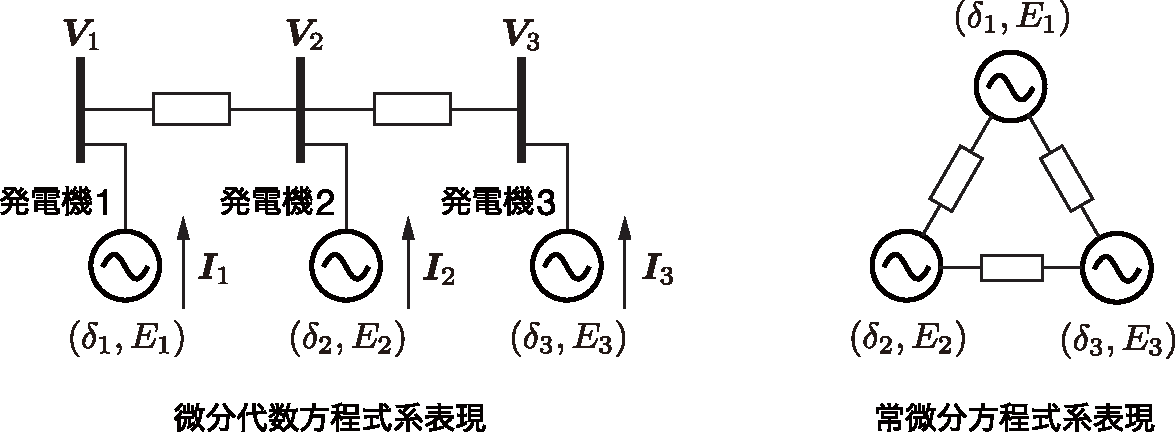
\includegraphics[width = .85\linewidth]{figs/kronredgen}
\medskip
\caption{\textbf{Changes in bond structure due to Kron reduction}}
\label{fig:krongen}
\medskip
\end{figure}


In addition, though the admittance matrix $\bm{Y}$ is a sparce matrix that reflects the graph structure of the power grid, the reduced admittance matrix $\bm{Y}^{\rm red}$ in Equation \ref{eq:krondyn} is usually not a sparce matrix.
%\footnote{
%要素の多くに0をもつ行列を\textbf{疎行列}(sparse matrix)と呼ぶ。
%逆に, ほとんどの要素に0でない値をもつ行列を\textbf{密行列}(dense matrix)と呼ぶ。
%ただし, どの程度の要素が0であれば疎行列と呼ぶかは文脈に依る。
%対角行列でない疎行列の逆行列は, 一般に密行列となる。
%}。
Therefore, please note that an ordinary differential equation system of Equation \ref{eq:krondyn} has a combined structure in which the internal state of all generators densely interact (\ref{fig:krongen}).
Let us confirm this fact with numerical examples along with the behavior of the electrical power system model. 

\begin{COLUMN}
\noindent \textbf{Sparse and dense matrices}:
A matrix with many 0 elements is called a \textbf{sparse matrix}.
In contrast, a matrix with almost no 0 elements is called a \textbf{dense matrix}.
However, how many 0 elements are necessary to call a matrix sparse matrix depends on the context.
The inverse matrix of a sparse matrix that is not a diagonal matrix is usually a dense matrix.
\end{COLUMN}


\begin{table}[h]
\medskip
 \caption{\textbf{Physical constants of the generator model}}
 \label{table:genparams}
 \centering
  \begin{tabular}{cccccc}
   \hline
$i$ &  $M_i$~[s] & $D_i$~[pu] & $\tau_i$~[s] & $\Xsi$~[pu] & $\Xti$~[pu] \\
   \hline \hline
1 & 100 & 10 & 5.14 & 1.569 & 0.936 \\
   \hline
2 & 18 & 10 & 5.90 & 1.651 & 0.911 \\
   \hline
3 & 12 & 10 & 8.97 & 1.220 & 0.667 \\
   \hline
  \end{tabular}
\end{table}

\begin{table}[h]
\medskip
 \caption{\textbf{Steady-state values of external inputs and internal conditions of the generator}}
 \label{table:gensteady}
 \centering
  \begin{tabular}{ccccccccccccccccc}
   \hline
$i$ &  $P_{{\rm mech}i}^{\star}$~[pu] & $V_{{\rm filed}i}^{\star}$~[pu] & $\delta_i^{\star}$~[rad] & $\Delta \omega_i^{\star}$~[pu] & $E_i^{\star}$~[pu] \\
   \hline \hline
1 & $-0.5623$ & 1.5132 & 0.4656 & 0 & 1.4363 \\
2 & 0.8832 & 2.2216 & 1.0903 & 0 & 1.8095 \\
3 & $-0.3160$ & 0.9198 & 0.6067 & 0 & 1.1030 \\
   \hline
  \end{tabular}
\end{table}


\begin{example}{Behavior of an electrical power system model where a generator bus is reduced}\label{ex:Kronode}
Let us consider an electrical power system model consisting of three bus bars as discussed in Example \ref{ex:derY}. 
Here, the one-axis generator model that was explained in Section \ref{sec:genfund} is connected to each bus bar. 
In other words, the electrical power system model can be drawn as shown in the left image in \ref{fig:krongen}. 
For the physical constant of the generators, values from \ref{table:genparams} are used. 
Since the system frequency is set to 60 [Hz], the value of $\omega_0$ is $120\pi$.


The admittance of the two transmission lines is set as:
\begin{align}\label{eq:defadpara}
\bm{y}_{12} = 1.3652 - \bm{j} 11.6041, \qquad
\bm{y}_{23} = 1.9422 - \bm{j} 10.5107
\end{align}
In this manner, the admittance matrix of the power grid in Equation \ref{eq:exY} is obtained.
In addition, if we calculate the real part (reduced conductance matrix) and the imaginary part (reduced susceptance matrix) of the reduced admittance matrix $\bm{Y}^{\rm red}$ of Equation \ref{eq:Yred}, 
the following is obtained:

\begin{align*}
\spliteq{
G^{\rm red}&=
\mat{
0.0073  & 0.0005 & -0.0079  \\
0.0005  & 0.0041 & -0.0046  \\
-0.0079 & -0.0046 & 0.0125 
}, \\
B^{\rm red}&=
\mat{
- 0.3716 & - 0.3167 & -0.3800  \\
- 0.3167 & - 0.3550 & - 0.4260  \\
- 0.3800 & - 0.4260 & - 0.6933
}
}
\end{align*}
%\[
%\bm{Y}^{\rm red}=
%\mat{
%0.0073 - \bm{j} 0.3716 & 0.0005 - \bm{j} 0.3167 & -0.0079 -  \bm{j} 0.3800  \\
%0.0005 - \bm{j} 0.3167 & 0.0041 - \bm{j} 0.3550 & -0.0046 -  \bm{j} 0.4260  \\
%-0.0079 -  \bm{j} 0.3800 & -0.0046 -  \bm{j} 0.4260 & 0.0125 -  \bm{j} 0.6933
%}
%\]
%\[
%\bm{Y}^{\rm red}=
%\mat{
%7.3\times 10^{-3} - \bm{j} 0.3716 & 0.5\times 10^{-3} - \bm{j} 0.3167 & -7.9\times 10^{-3} -  \bm{j} 0.3800  \\
%0.5\times 10^{-3} - \bm{j} 0.3167 & 4.1\times 10^{-3} - \bm{j} 0.3550 & -4.6\times 10^{-3} -  \bm{j} 0.4260  \\
%-7.9\times 10^{-3} -  \bm{j} 0.3800 & -4.6\times 10^{-3} -  \bm{j} 0.4260 & 12.5\times 10^{-3} -  \bm{j} 0.6933
%}
%\]
It shows that both are dense matrices.
This dense structure corresponds to the right image of \ref{fig:krongen}.



Next, let us calculate the time response of an ordinary differential equation system model of Equation \ref{eq:krondyn}.
Below, we obtain the initial response when the external input, mechanical torque and field voltage are fixed as constant.
In this example, we use the steady state calculation method, which will be discussed in Section \ref{sec:powflow},
and assume that the external input of the electrical power system model and steady value of the internal state have been obtained in advance.
Specifically, the external input, mechanical torque and field voltage are set to constants in the first and second columns of \ref{table:gensteady}.
In this case, the steady value of the internal state of the electrical power system are values in the third to fifth columns in \ref{table:gensteady}.
%\[
%\mat{
%P_{{\rm mech}1}^{\star} \\
%P_{{\rm mech}2}^{\star} \\
%P_{{\rm mech}3}^{\star} 
%}
%=
%\mat{
%-0.5623\\
%0.8832\\
%-0.3160
%}, \qquad
%\mat{
%V_{{\rm filed}1}^{\star} \\
%V_{{\rm filed}2}^{\star} \\
%V_{{\rm filed}3}^{\star} 
%}
%=
%\mat{
%1.5132\\
%2.2216\\
%0.9198
%}
%\]
%で与えられる場合には, 電力系統モデルの内部状態の定常値が
%\[
%\mat{
%\delta_1^{\star} \\
%\delta_2^{\star} \\
%\delta_3^{\star} 
%}
%=
%\mat{
%0.4656 \\
%1.0903 \\
%0.6067
%},\qquad
%\mat{
%\Delta \omega_1^{\star} \\
%\Delta \omega_2^{\star} \\
%\Delta \omega_3^{\star} 
%}
%=
%\mat{
%0 \\
%0 \\
%0
%},\qquad
%\mat{
%E^{\star}_1 \\
%E^{\star}_2 \\
%E^{\star}_3 
%}
%=
%\mat{
%1.4363 \\
%1.8095 \\
%1.1030
%}
%\]
%となることを前提にする。
These steady values are one of the solutions that satisfy simultaneous equations:
\begin{align*}
\simode{
0 &= %\textstyle
 - f_i \left( \delta^{\star},E^{\star} \right)
+P_{{\rm mech}i}^{\star}
\\
0 & = %\textstyle
 -  \tfrac{ \Xsi }{\Xti }  E_i^{\star}  + \left(
\Xsi - \Xti
\right)
g_i \left( \delta^{\star},E^{\star} \right)
+ V_{{\rm field}i}^{\star}
}
\qquad
 i \in \{1,2,3\}
\end{align*}
where $\delta^{\star}$ and $E^{\star}$ are vectors with $\delta_i^{\star}$ and $E_i^{\star}$.
Functions $f_i$ and $g_i$ are defined by Equation \ref{eq:figidef}.


First, let us consider a situation where the steady value is perturbed to set the initial value.
Specifically:
\begin{align}\label{eq:exdelE0}
\mat{
\delta_1(0) \\
\delta_2(0) \\
\delta_3(0) 
}
 =
\mat{
\delta_1^{\star} + \tfrac{\pi}{6} \\
\delta_2^{\star} \\
\delta_3^{\star} 
},\qquad
%\mat{
%\Delta \omega_1(0) \\
%\Delta \omega_2(0) \\
%\Delta \omega_3(0) 
%}
%=
%\mat{
%\Delta \omega_1^{\star} \\
%\Delta \omega_2^{\star} \\
%\Delta \omega_3^{\star} 
%}, \\
\mat{
E_1(0) \\
E_2(0) \\
E_3 (0)
}
 =
\mat{
E^{\star}_1 +0.1 \\
E^{\star}_2 \\
E^{\star}_3 
}
\end{align}
where the initial value of the frequency deviation is 0. The time response of the electrical power system model at this time is shown in \ref{fig:Kron0}.
This figure shows that, after frequency deviation and rotor argument were perturbed for about 15 seconds, they asymptotically converge to the original steady state.
However, since only the relative difference among generators is meaningful in the rotor argument, the convergence value of the rotor argument shifts by a constant from the original steady value.
In other words, for a certain constant $c_0$:
\[
\lim_{t\rightarrow \infty} \delta_i(t) = \delta_i^{\star} +c_0,\qquad
\forall i \in \{1,2,3\}
\]
For any value of $c_0$, the steady value is essentially equivalent.
The voltage phasor of the bus bar shown in \ref{fig:Kron0} can be calculated independently of the internal state of the generators using the relationship in Equation \ref{eq:colVi}.
Similarly, the active and reactive power can be calculated independently using Equation \ref{eq:PiQis2}.
Furthermore, since the system frequency is set to 60 [Hz], $5\times 10^{-3}$~[pu] of the frequency deviation is equal to 0.3 [Hz].

Next, let us consider a case wherein the value of the external input is perturbed.
Specifically, the mechanical torque of generator 1 is perturbed:
\[
\mat{
P_{{\rm mech}1}(t) \\
P_{{\rm mech}2}(t) \\
P_{{\rm mech}3}(t) 
}=
\mat{
P_{{\rm mech}1}^{\star} +0.05\\
P_{{\rm mech}2}^{\star} \\
P_{{\rm mech}3}^{\star} 
}
\]
\ref{fig:KronP} shows the time response of the electrical power system model under this condition.
The initial value is set to be the same as the value in Equation \ref{eq:exdelE0}.
The phase of the rotor argument and the voltage phasor of the bus bar voltage phasor express the remainder when divided by $2\pi$.
In this case, the frequency deviation does not become 0 under a steady state, and the rotor argument where it has been integrated continues to change constantly.
\ref{fig:KronV} shows the time response of the electrical power system model when field voltage of generator 1 is similarly perturbed:
\[
\mat{
V_{{\rm filed}1}(t) \\
V_{{\rm filed}2}(t) \\
V_{{\rm filed}3}(t) 
}=
\mat{
V_{{\rm filed}1}^{\star} +0.5 \\
V_{{\rm filed}2}^{\star} \\
V_{{\rm filed}3}^{\star} 
}
\]
In this situation as well, the frequency deviation in a steady state does not become 0.
As such, to calculate the time response of an electrical power system model, not only must the initial value be set to the appropriate values, but the external inputs, mechanical torque and field voltage as well.
\end{example}


Since Equation \ref{eq:krondyn} is an ordinary differential equation system model, by using a differential equation solver, which is a standard add-on in MATLAB, its behavior can be numerically simulated.
However, as shown in example \ref{ex:Kronode}, unless the value of the mechanical torque and the field voltage are set appropriately, the frequency deviation of each generator under a steady state does not become 0, and the rotor argument constantly deviates from the reference coordinates.
Thus, to perform a numerical simulation that is realistically meaningful, a process to calculate valid equilibrium points and initial values is necessary.
These details will be explained in Chapter \ref{chap:numcal}.

\begin{figure}[t]
  \centering
  {
  \begin{minipage}{0.49\linewidth}
    \centering
    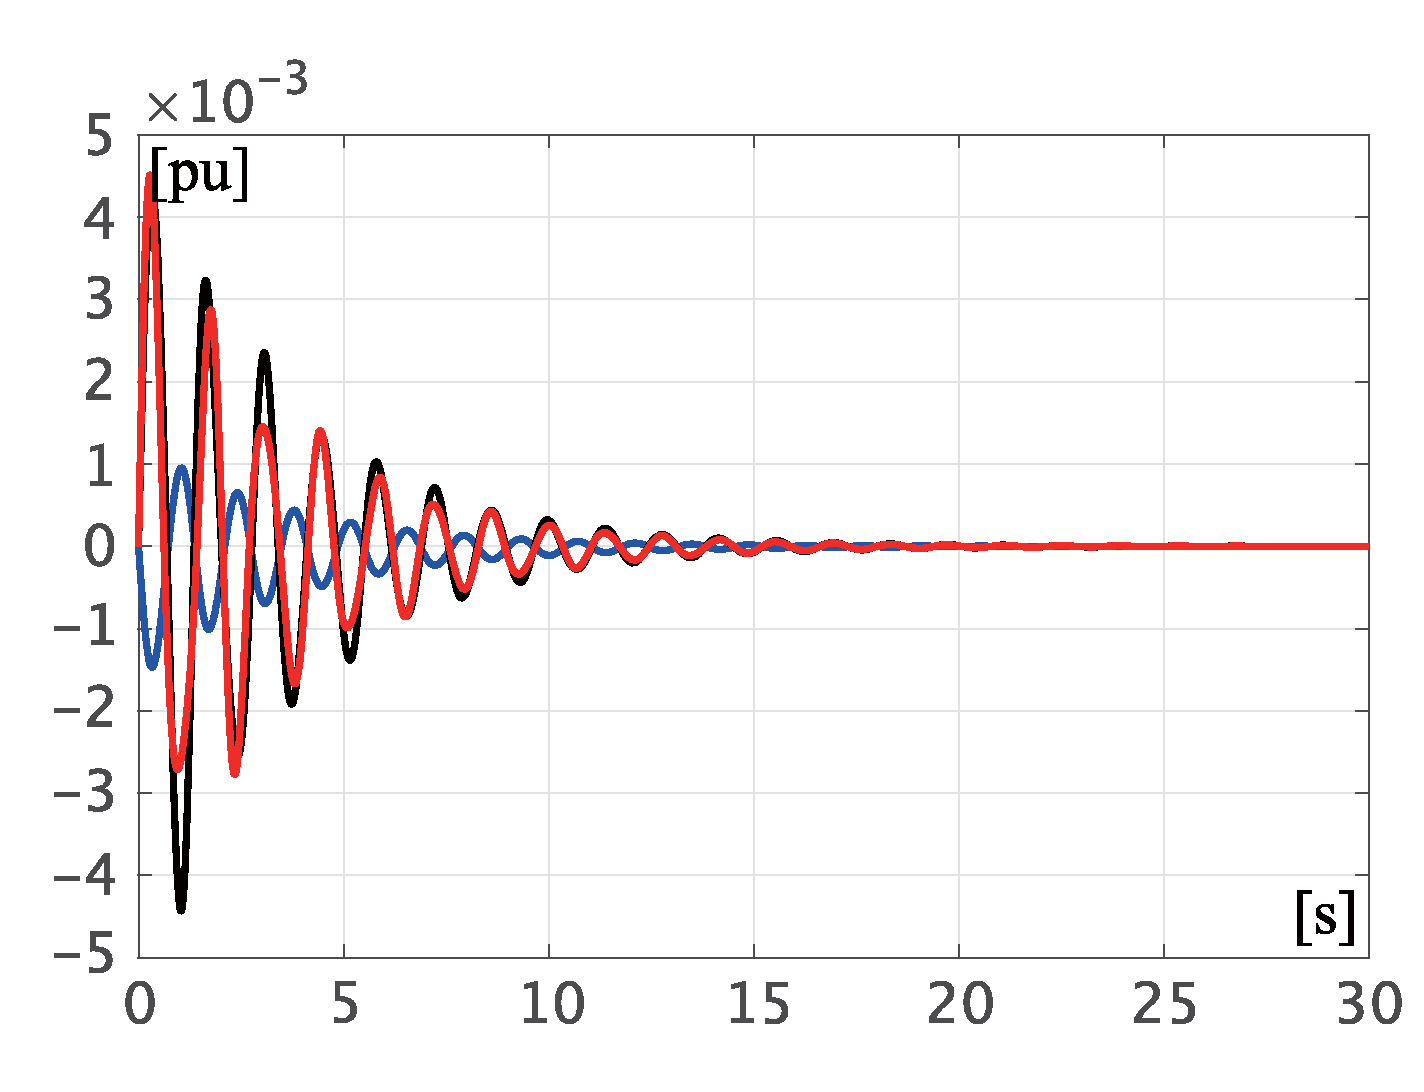
\includegraphics[width = 1.0\linewidth]{figs/Domega0}
    \subcaption{ $\Delta \omega_i$}
    \medskip
  \end{minipage}
  \begin{minipage}{0.49\linewidth}
    \centering
    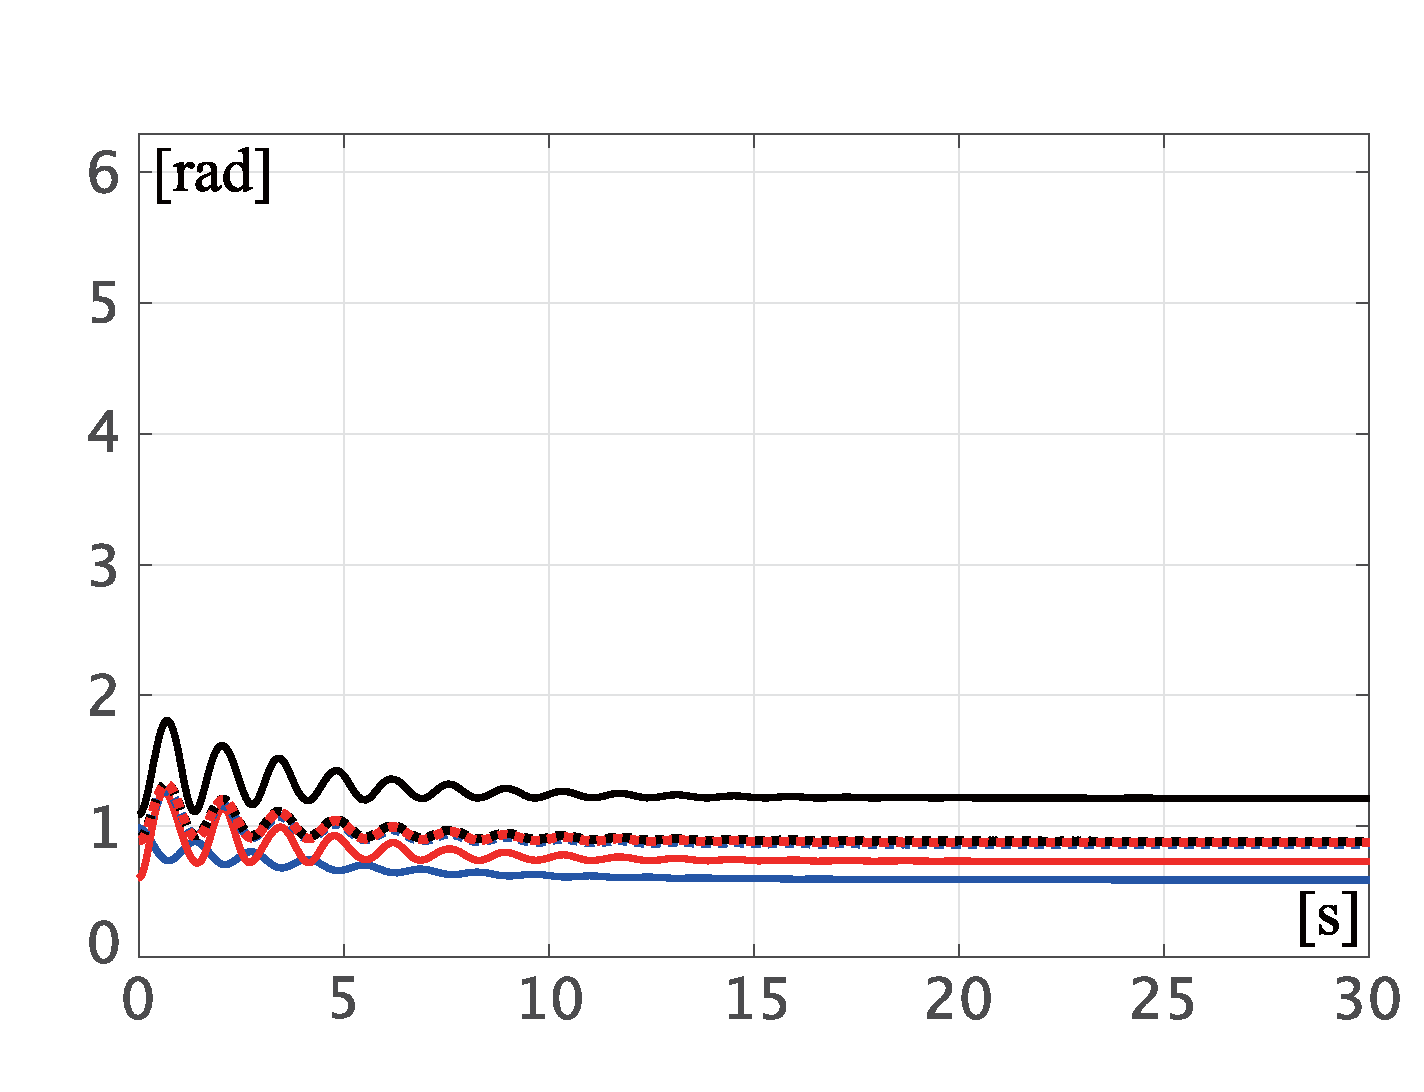
\includegraphics[width = 1.0\linewidth]{figs/delangV0}
    \subcaption{ Solid line: (1)$\delta_i$, Dashed line: $\angle \bm{V}_i$ }
    \medskip
  \end{minipage}
 \begin{minipage}{0.49\linewidth}
    \centering
    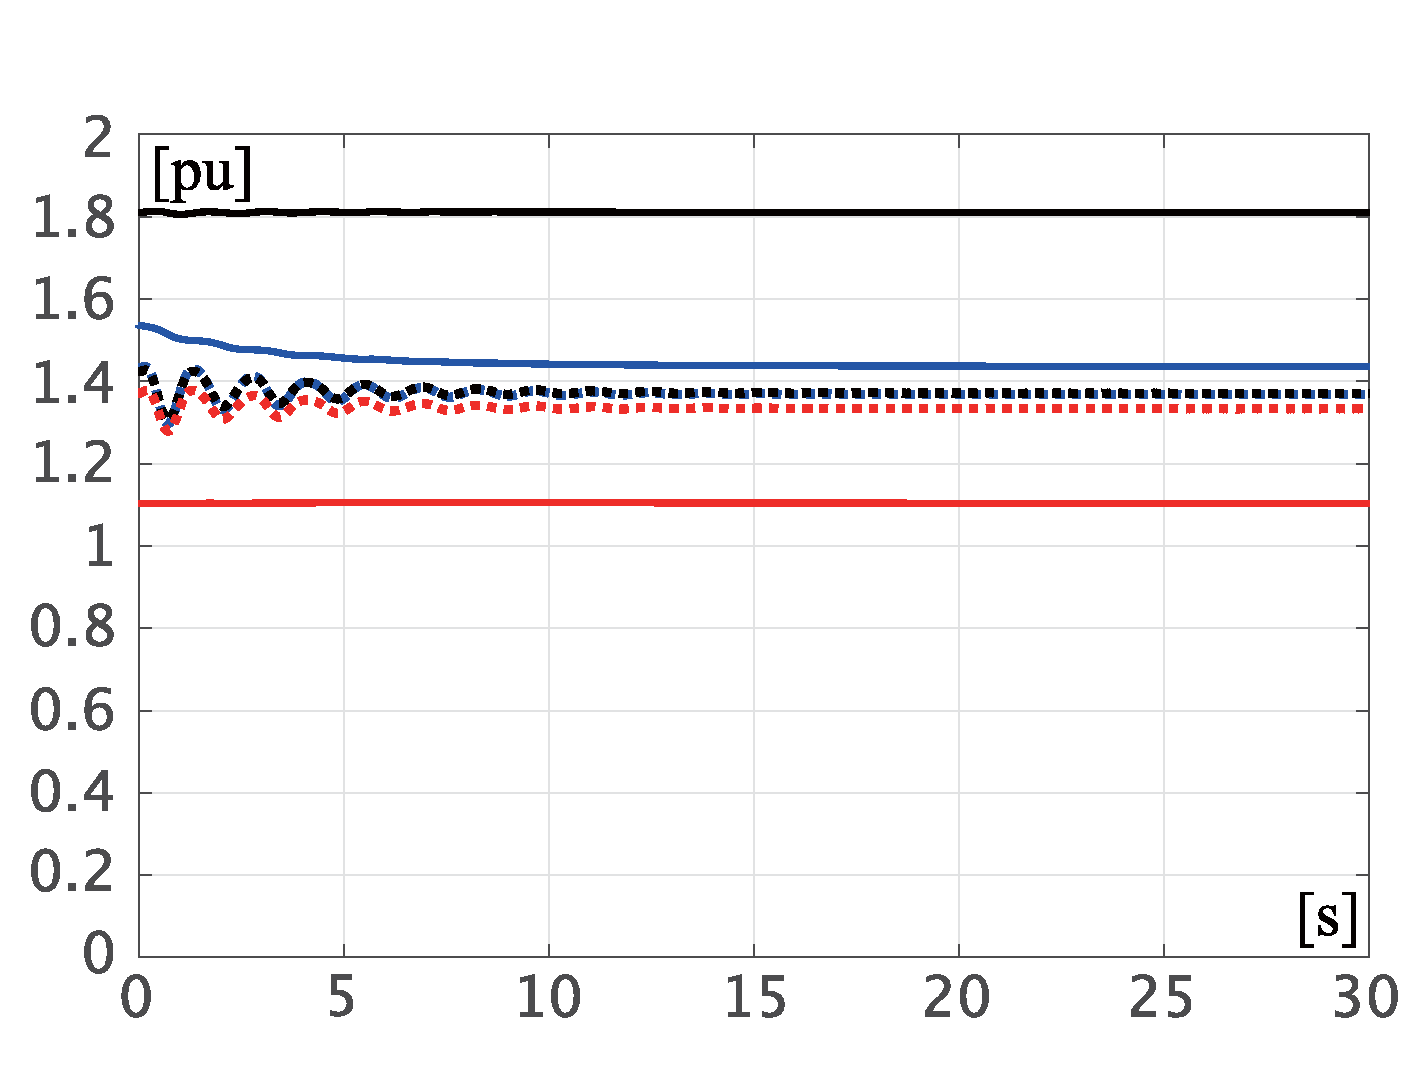
\includegraphics[width = 1.0\linewidth]{figs/EabsV0}
    \subcaption{ Solid line: $E_i$, Dashed line: $|\bm{V}_i|$ }
    \medskip
  \end{minipage}
  \begin{minipage}{0.49\linewidth}
    \centering
    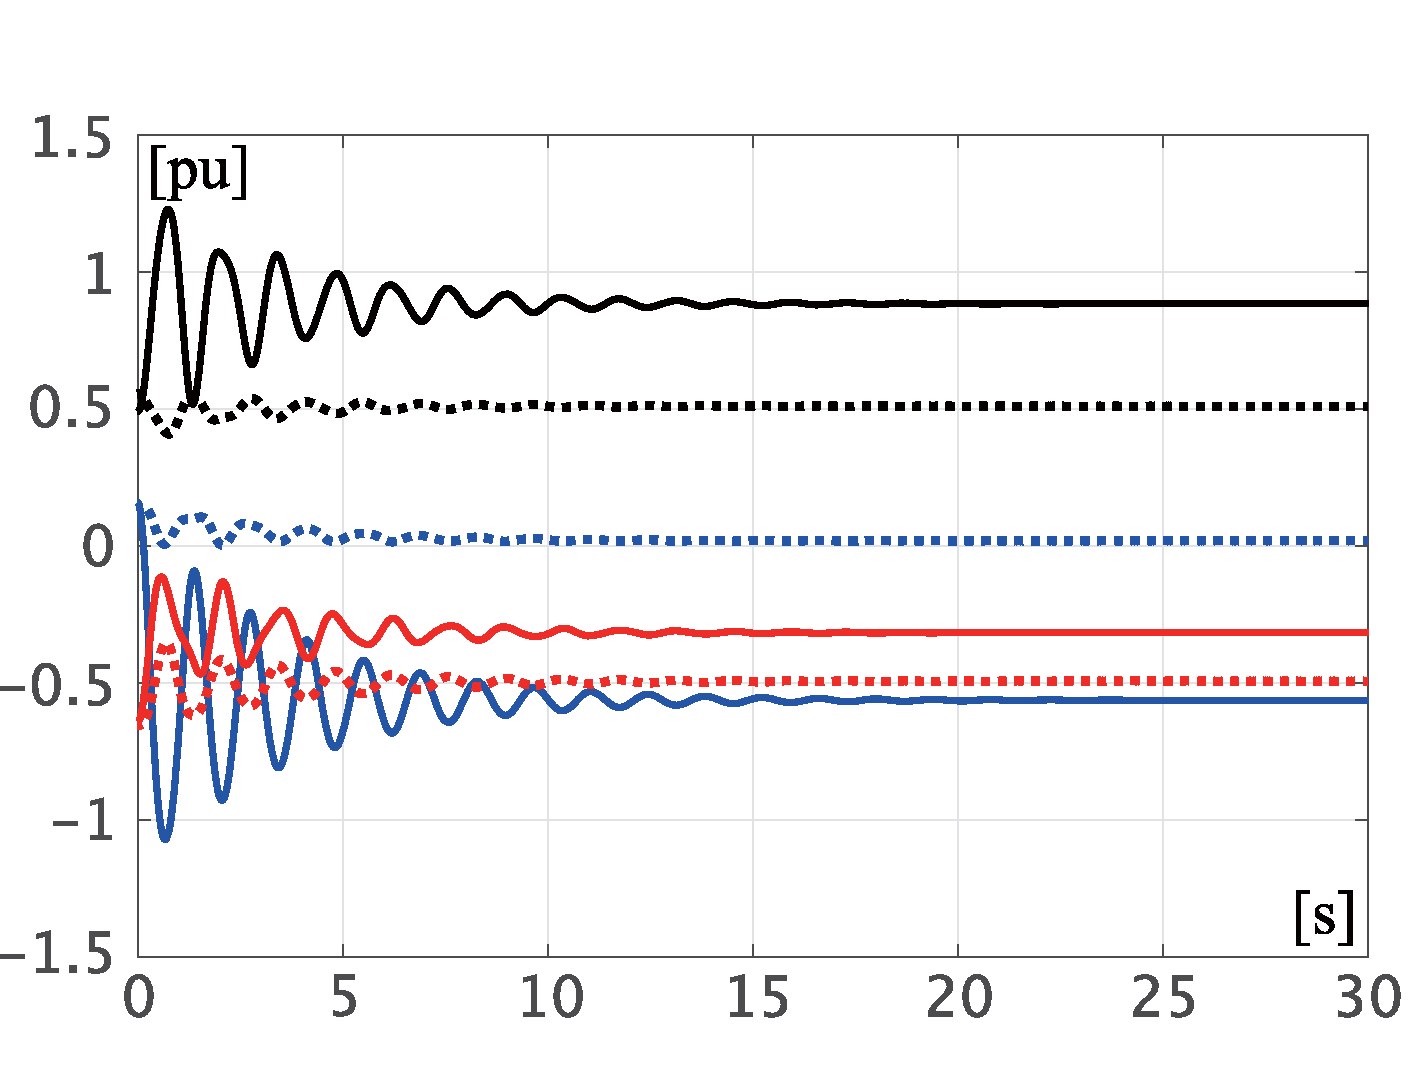
\includegraphics[width = 1.0\linewidth]{figs/PQ0}
    \subcaption{ Solid line: $P_i$, Dashed line: $Q_i$ }
    \medskip
  \end{minipage}
  }
  \medskip
  \caption{\textbf{Time response when perturbation is added to the initial value}
  \\  \centering((Blue: Bus 1, Black: Bus 2, Red: Bus 3))}
  \label{fig:Kron0}
\medskip
\end{figure}

\begin{figure}[t]
  \centering
  {
  \begin{minipage}{0.49\linewidth}
    \centering
    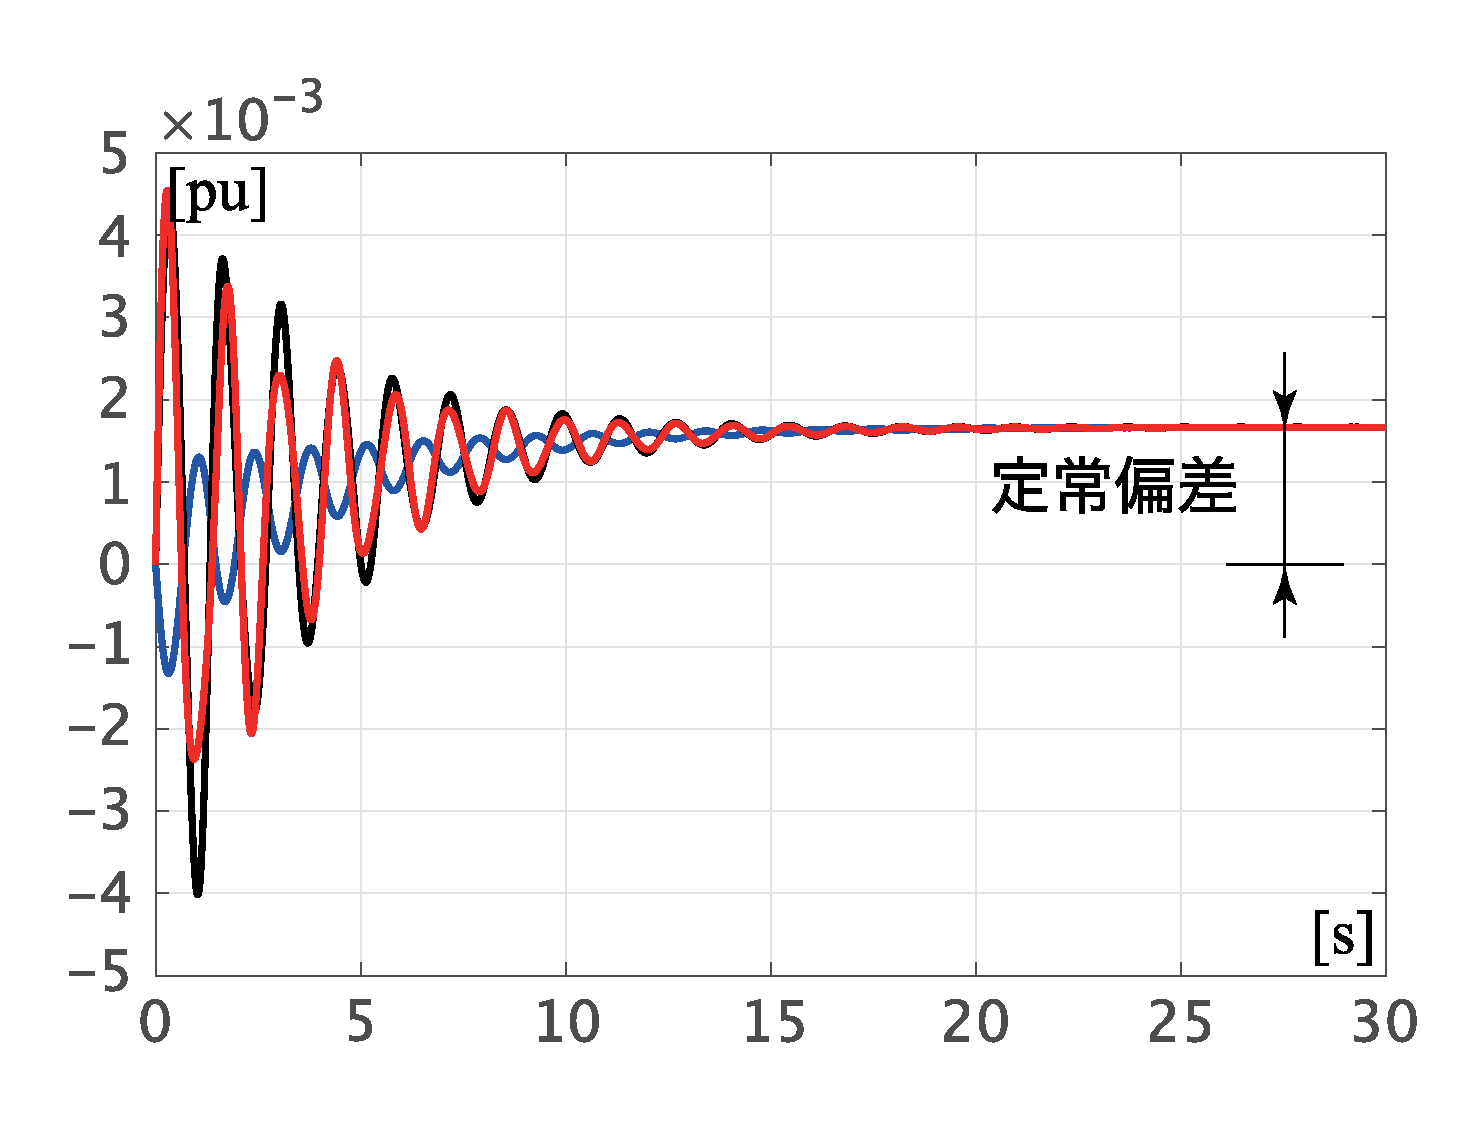
\includegraphics[width = 1.0\linewidth]{figs/DomegaP}
    \subcaption{ $\Delta \omega_i$ }
    \medskip
  \end{minipage}
  \begin{minipage}{0.49\linewidth}
    \centering
    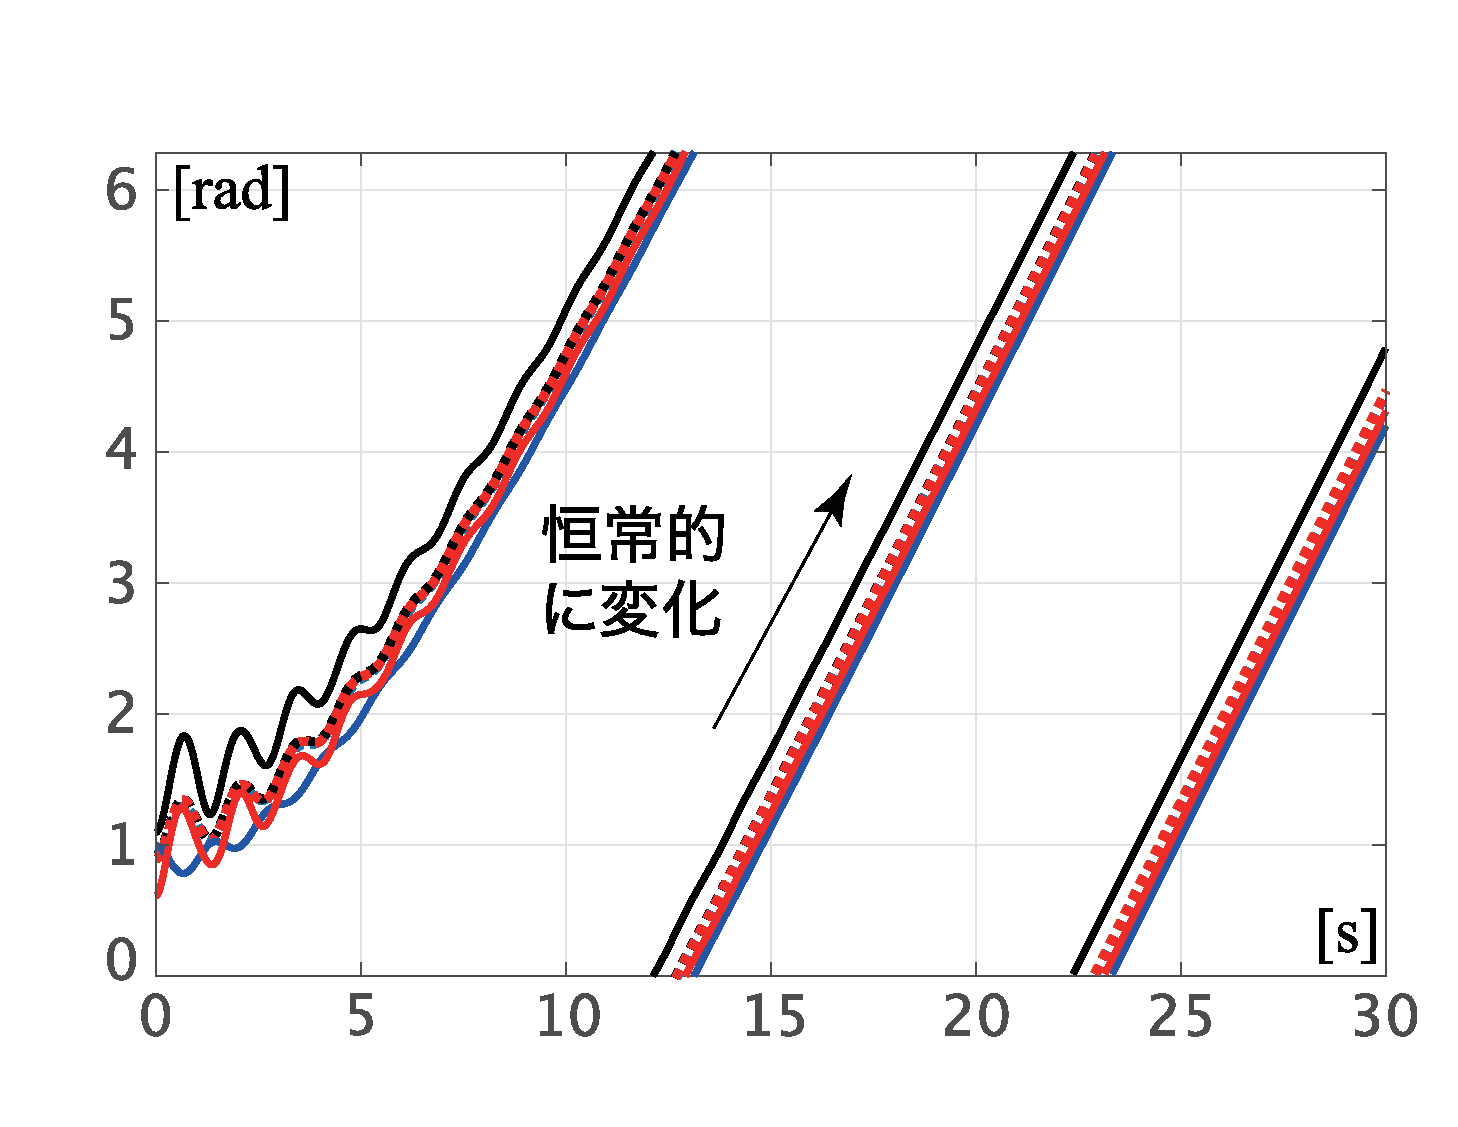
\includegraphics[width = 1.0\linewidth]{figs/delangVP}
    \subcaption{ Solid line: $\delta_i$, Dashed line:$\angle \bm{V}_i$ }
    \medskip
  \end{minipage}
 \begin{minipage}{0.49\linewidth}
    \centering
    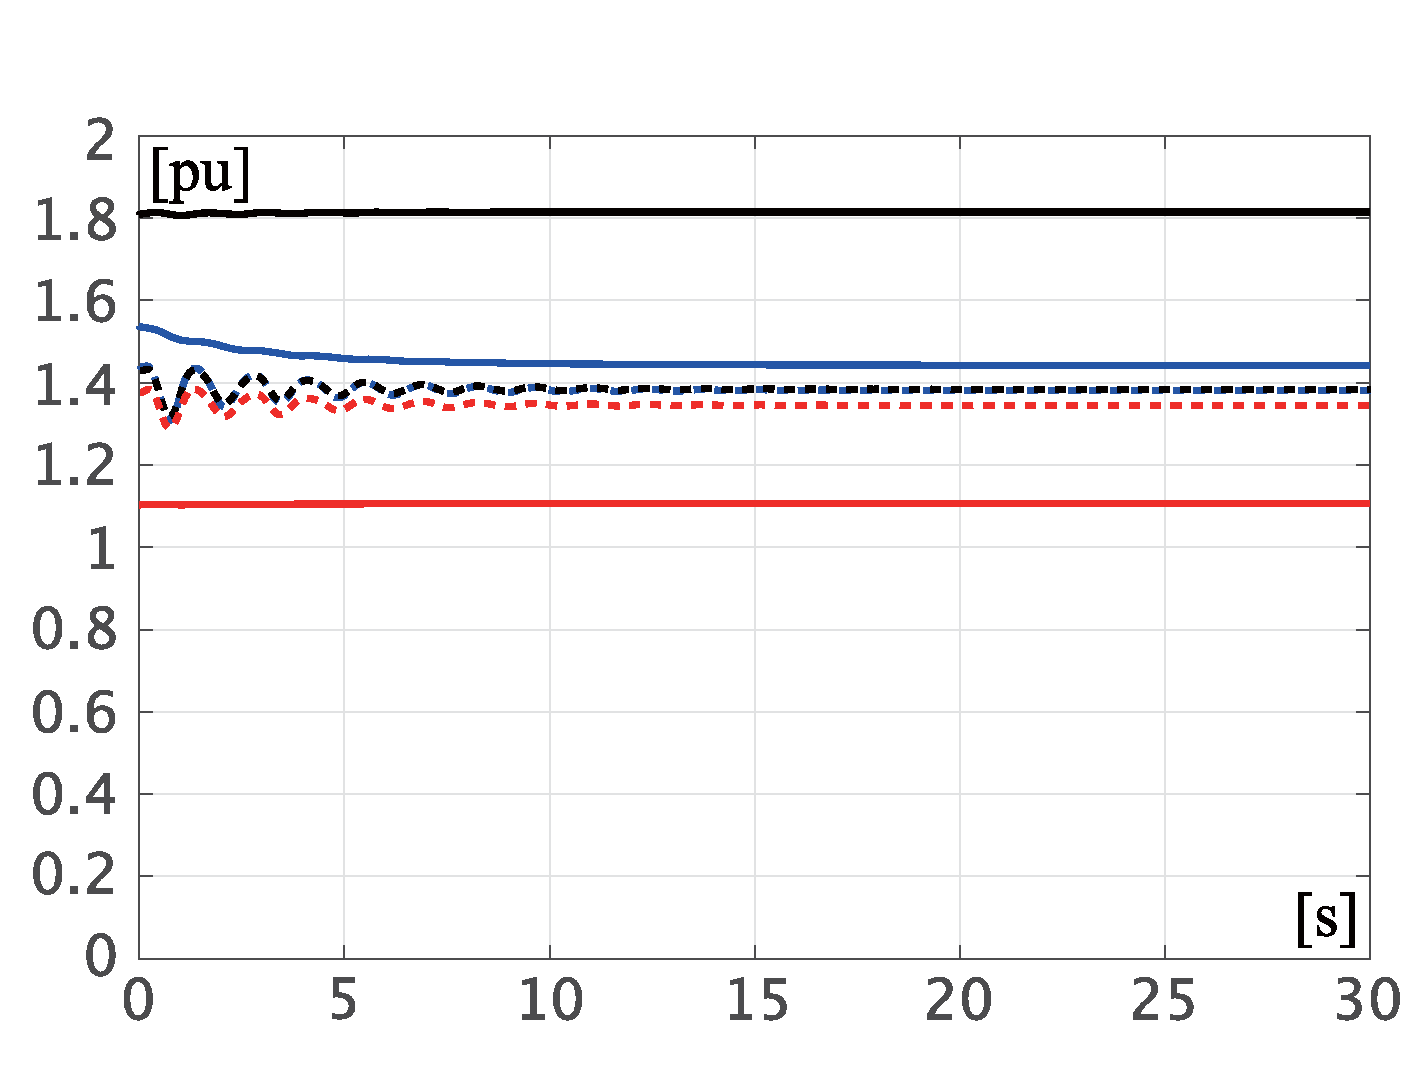
\includegraphics[width = 1.0\linewidth]{figs/EabsVP}
    \subcaption{ Solid line: $E_i$, Dashed line:$|\bm{V}_i|$ }
    \medskip
  \end{minipage}
  \begin{minipage}{0.49\linewidth}
    \centering
    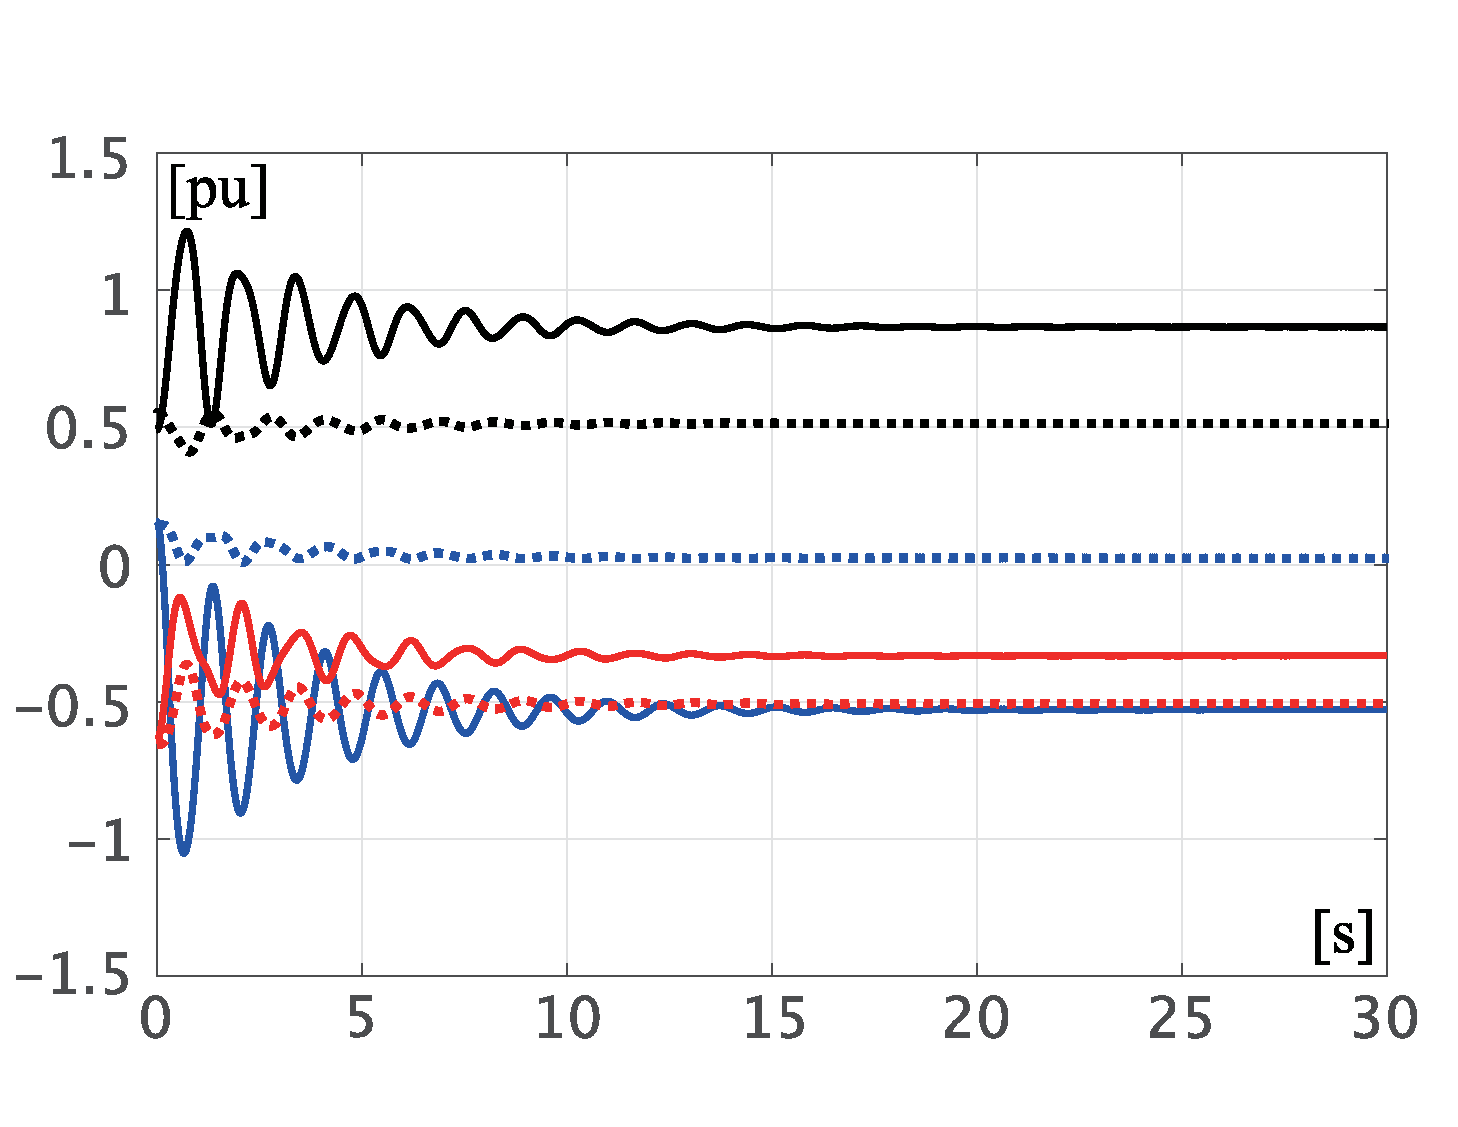
\includegraphics[width = 1.0\linewidth]{figs/PQP}
    \subcaption{ Solid line: $P_i$, Dashed line:$Q_i$ }
    \medskip
  \end{minipage}
  }
  \medskip
  \caption{\textbf{Time response when perturbation is added to machine input}
  \\  \centering(Blue: Bus 1, Black: Bus 2, Red: Bus 3)}
  \label{fig:KronP}
\medskip
\end{figure}

\begin{figure}[t]
  \centering
  {
  \begin{minipage}{0.49\linewidth}
    \centering
    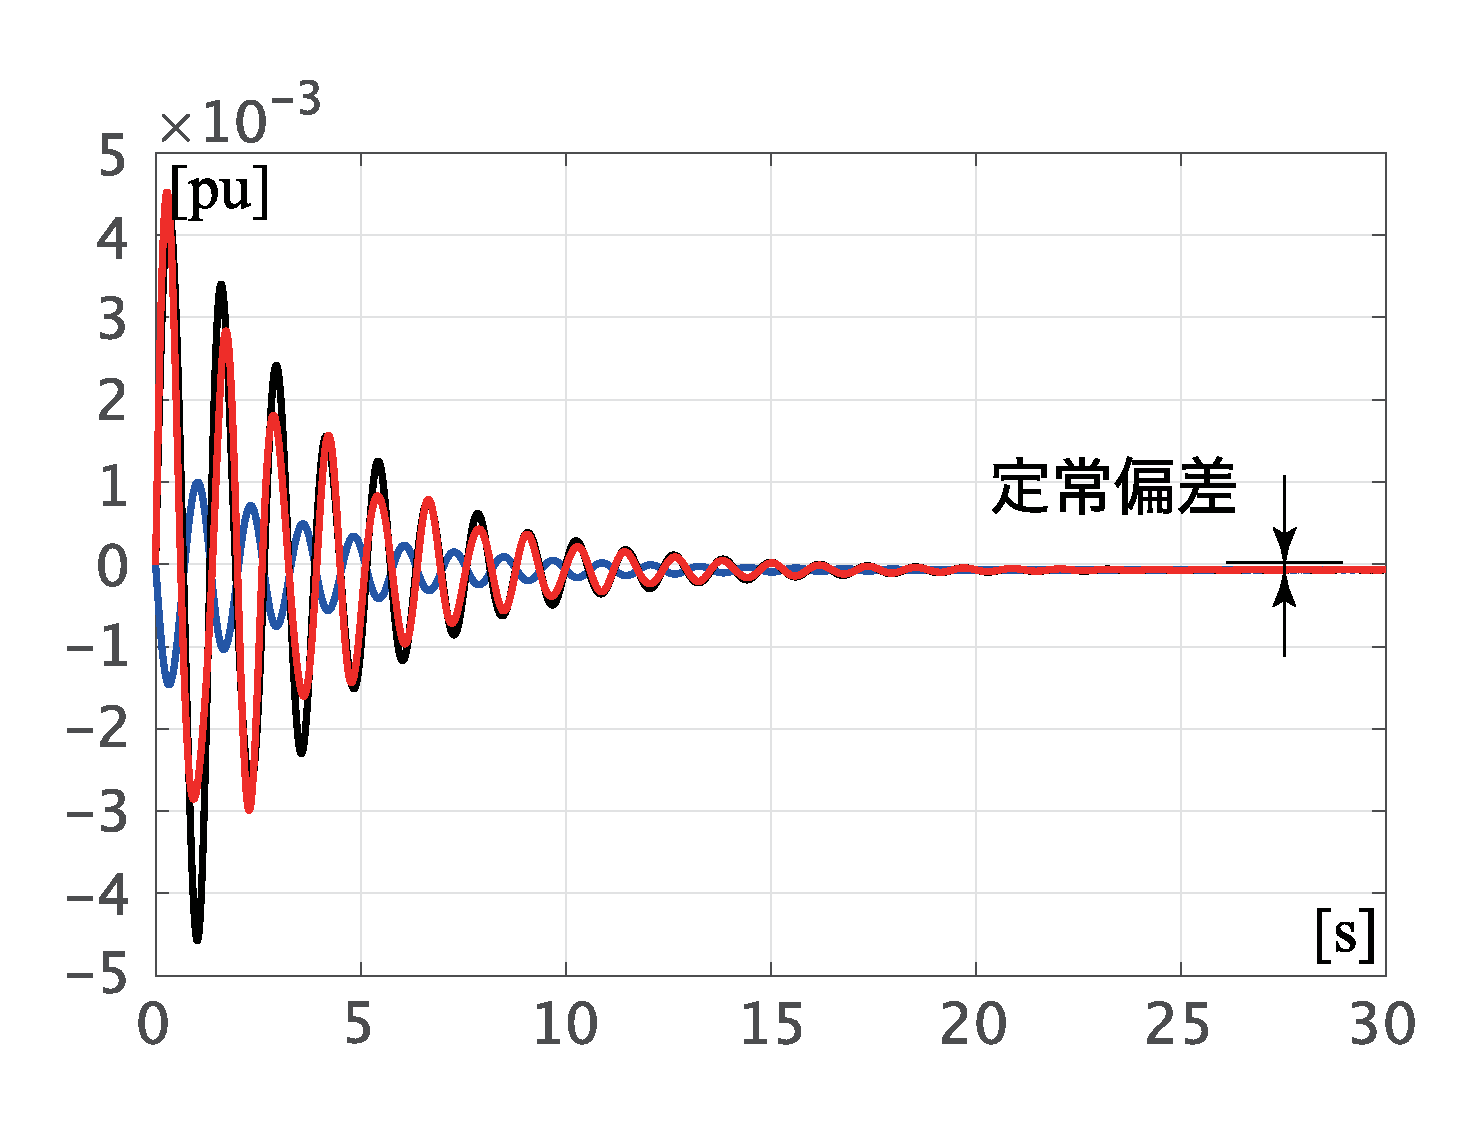
\includegraphics[width = 1.0\linewidth]{figs/DomegaV}
    \subcaption{ $\Delta \omega_i$ }
    \medskip
  \end{minipage}
  \begin{minipage}{0.49\linewidth}
    \centering
    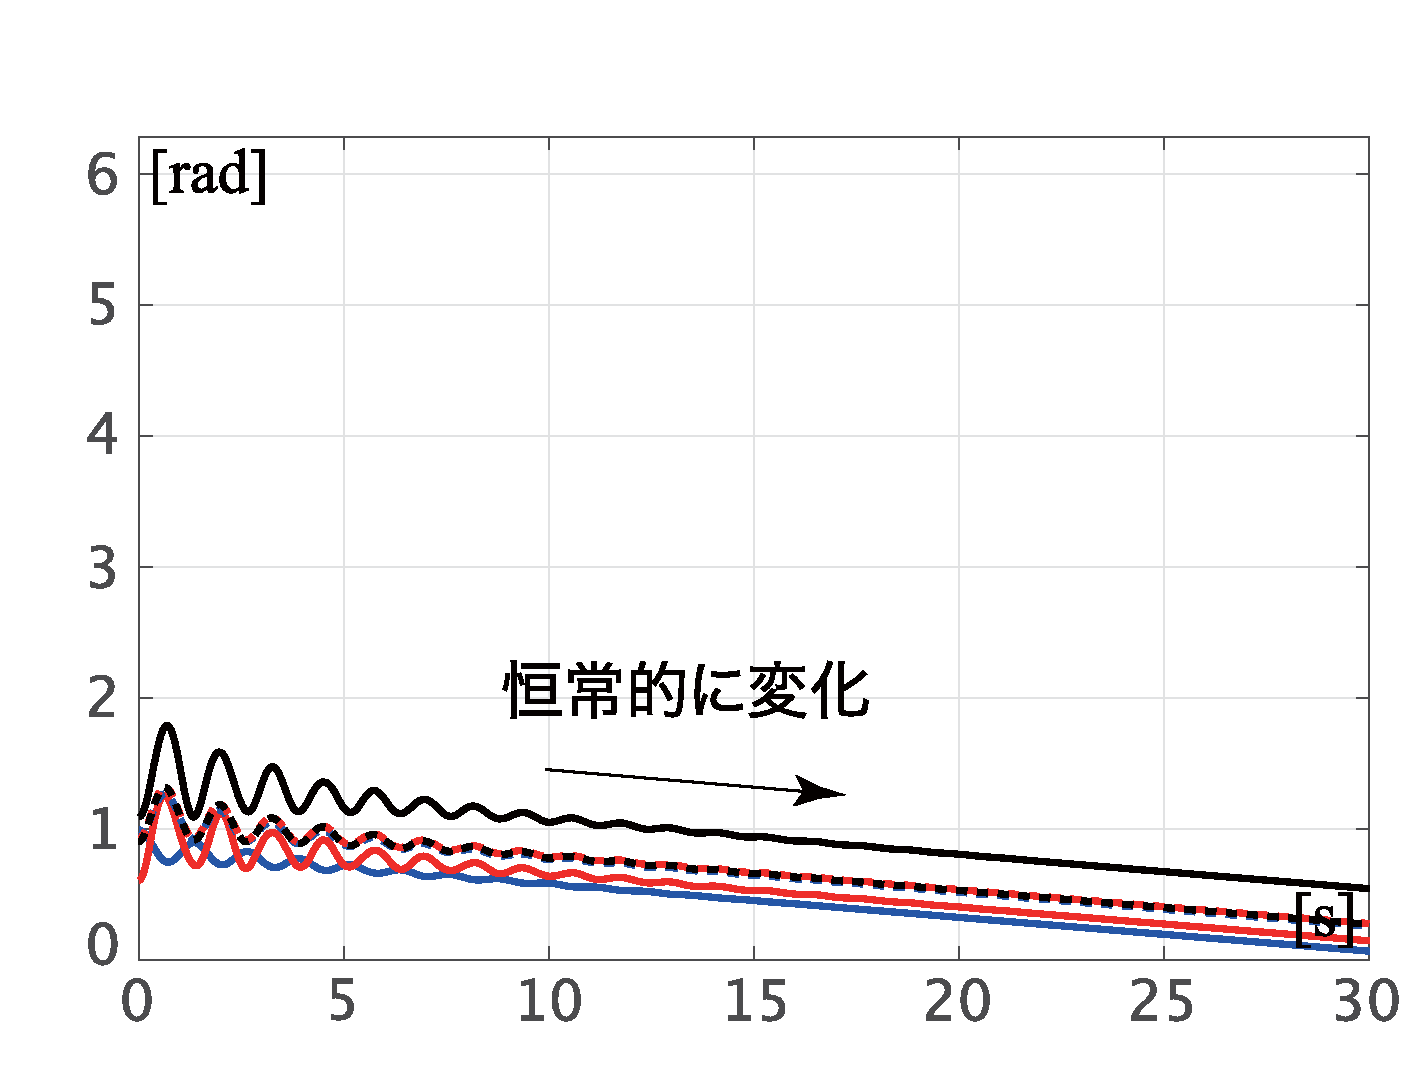
\includegraphics[width = 1.0\linewidth]{figs/delangVV}
    \subcaption{ Solid line: $\delta_i$, Dashed line:$\angle \bm{V}_i$ }
    \medskip
  \end{minipage}
 \begin{minipage}{0.49\linewidth}
    \centering
    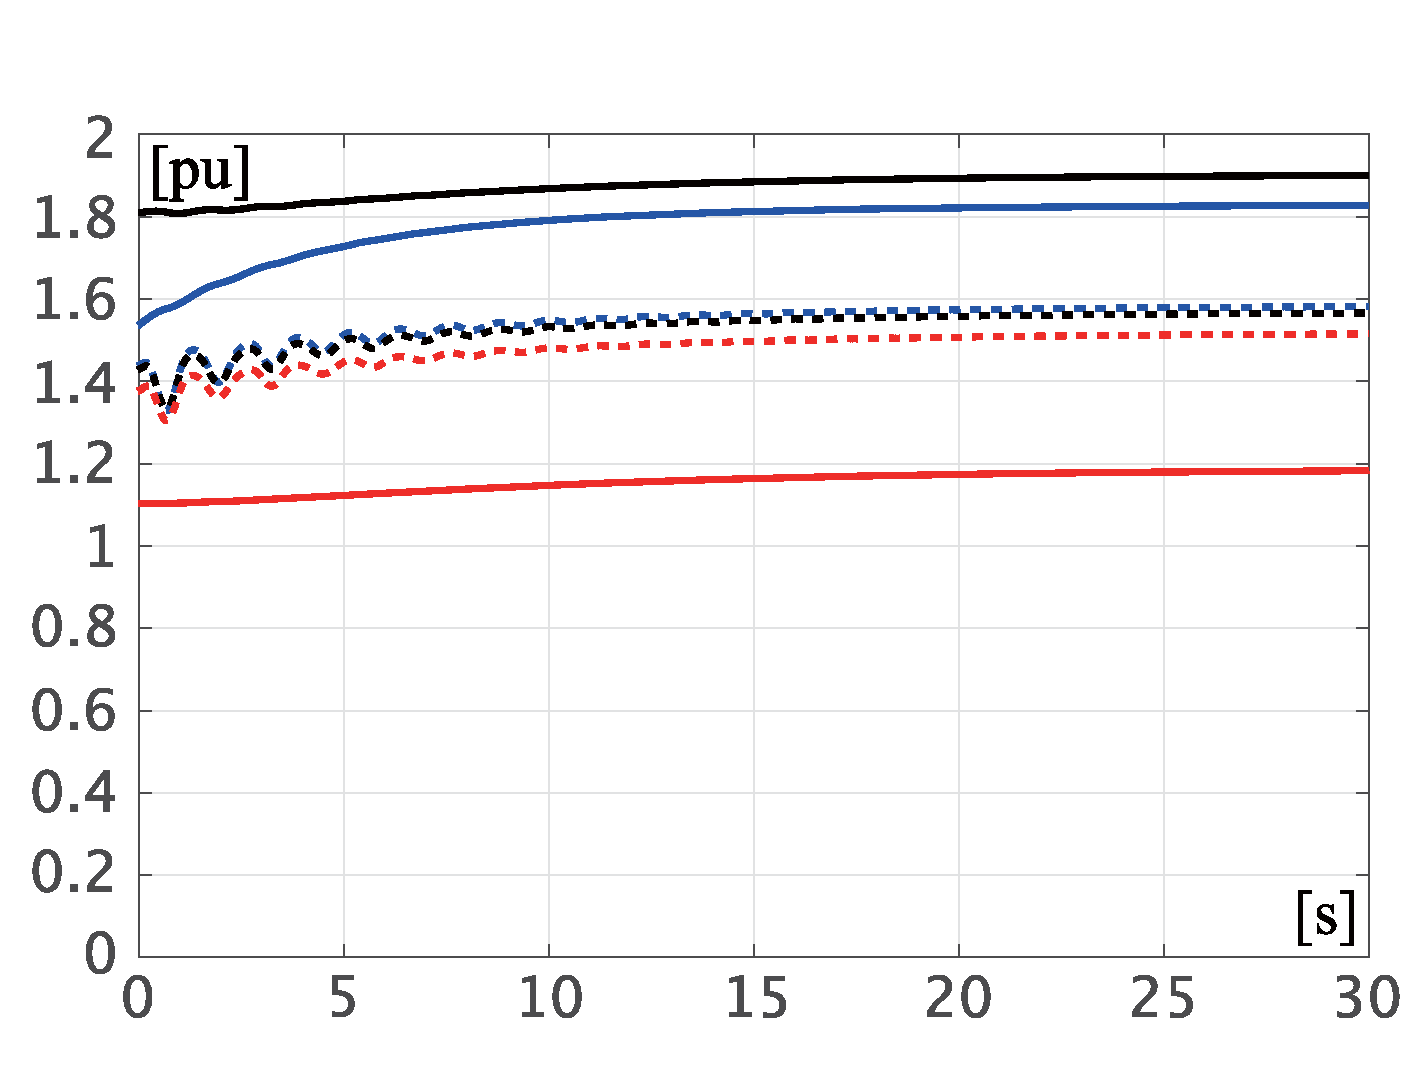
\includegraphics[width = 1.0\linewidth]{figs/EabsVV}
    \subcaption{ Solid line: $E_i$, Dashed line:$|\bm{V}_i|$ }
    \medskip
  \end{minipage}
  \begin{minipage}{0.49\linewidth}
    \centering
    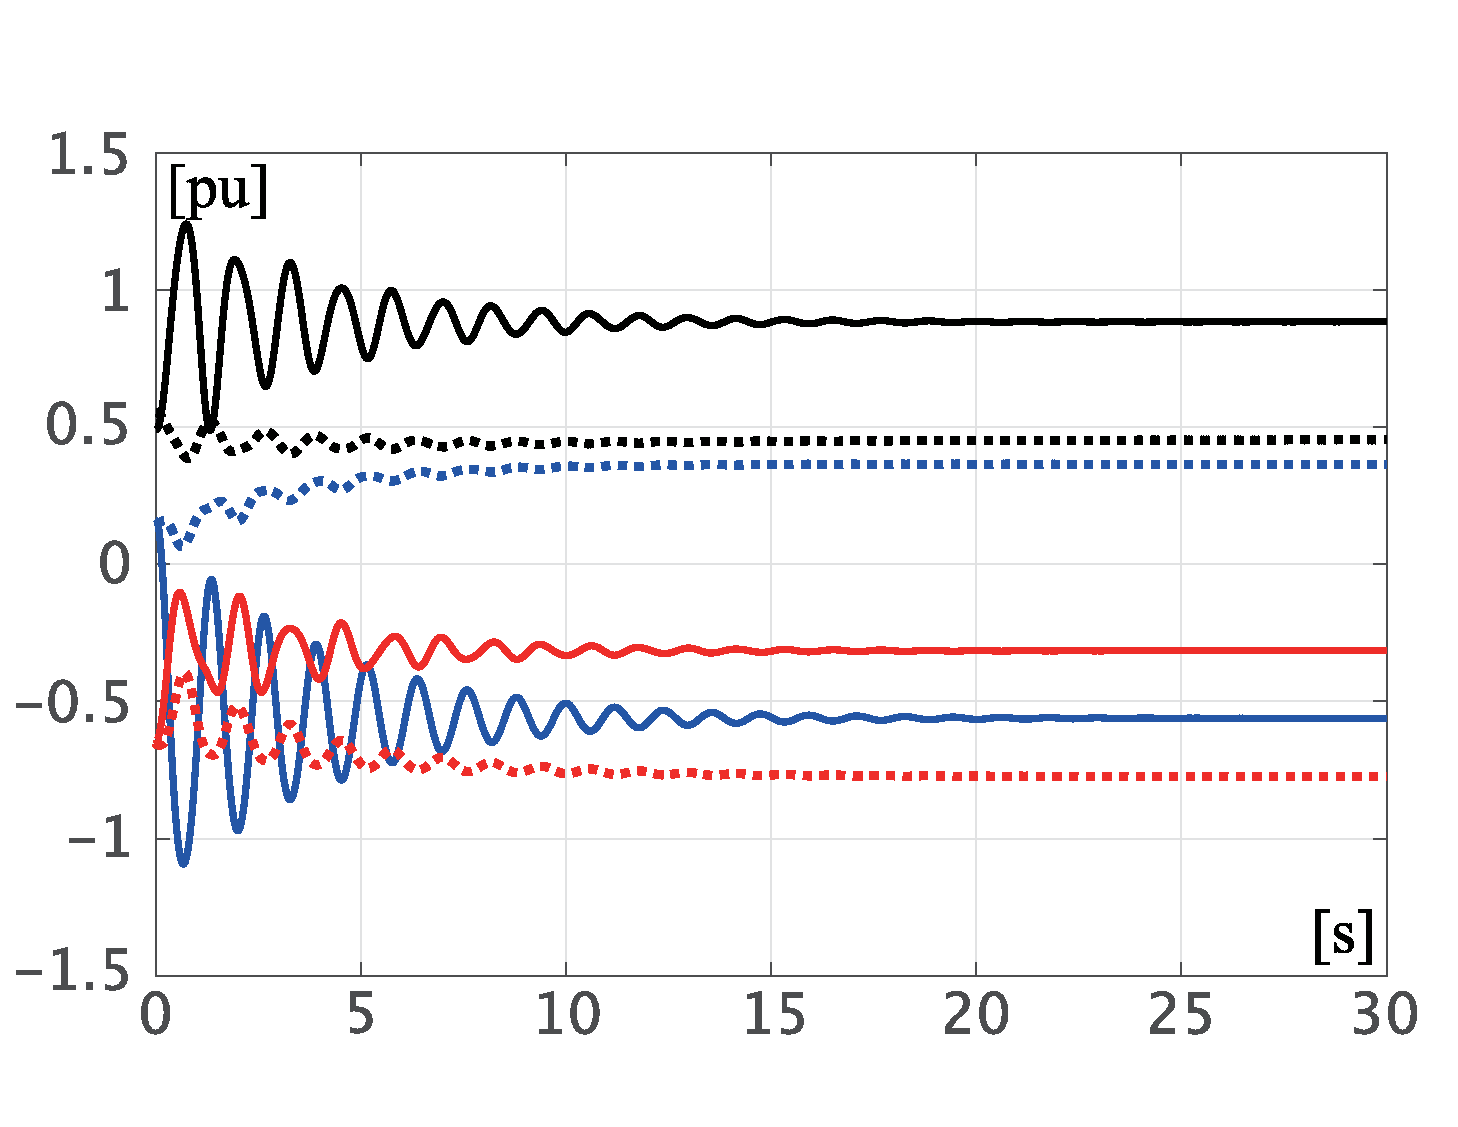
\includegraphics[width = 1.0\linewidth]{figs/PQV}
    \subcaption{ Solid line: $P_i$, Dashed line:$Q_i$ }
    \medskip
  \end{minipage}
  }
  \medskip
  \caption{\textbf{Time response when perturbation is applied to the field input}
  \\  \centering(Blue: Bus 1, Black: Bus 2, Red: Bus 3)}
  \label{fig:KronV}
\medskip
\end{figure}

\subsection{Derivation of the Kuramoto-type oscillator model}\label{sec:kuramod}

By applying Kron reduction of generator bus to the classical model explained in Section \ref{sec:genfund}, the Kuramoto-type oscillator model can be derived.
%\footnote{
%蔵本モデルは, 主に物理学の分野で解析されている非線形振動子の同期現象を記述する数理モデルであり, 幅広い応用をもつことが知られている\cite{kuramoto1975self,kuramoto2003chemical}。
%蔵本モデルを2次の非線形振動子系に拡張したモデルは, 電力系統の同期現象の解析にも応用されている\cite{dorfler2012synchronization,dorfler2013synchronization,nagata2014node,nishikawa2015comparative}。
%}
%。
Specifically, if we assume that the value of synchronous reactance $\Xsi$ and transient reactance $\Xti$ are equal, and field voltage $V_{{\rm field}i}$ is constant at $V_i^{\star}$, the internal voltage $E_i$ becomes $V_i^{\star}$ and is constant.
Therefore, the electrical power system model in which a generator is connected to each bus bar is expressed with a differential equation system model. 
\begin{align}\label{eq:clamod}
\simode{
\dot{\delta}_i&= \omega_0  \Delta \omega_i\\
M_i   \Delta \dot{\omega}_i&= 
 - D_i \Delta\omega_i - 
\hat{f}_i (\delta)
+P_{{\rm mech}i} 
}\qquad
i\in \mathcal{I}_{\rm G}
\end{align}
However, the nonlinear term is given by:
\[
\hat{f}_i (\delta):=
- V_i^{\star} \sum_{j=1}^{N}
V_j^{\star}\left(
B_{ij}^{\rm red}   \sfsin \delta_{ij}
-
G_{ij}^{\rm red}   \sfcos \delta_{ij}
\right)
\]
Function $\hat{f}_i (\delta)$ expresses the active power of a generator $i$.
An electrical power system model, where it is assumed that the conductance of a transmission line is 0; in other words, $G_{ij}^{\rm red}$ is 0, is occasionally used. 

\begin{COLUMN}
\red{Translated with DeepL}

\noindent\textbf{Kuramoto model}:

The following differential equation system with $N$ oscillators moving on the circumference
\[
\dot{\theta}_i = \omega_i - \frac{K}{N} \sum_{j=1}^N \sfsin (\theta_i - \theta_j),
\qquad
i=1,\ldots,N
\]
is called \textbf{Kuramoto model}. 
However, $\omega_i$ is a constant representing the intrinsic angular velocity of the oscillator $i$, and $K$ is a constant representing the bond strength. 
In general, the angular velocity of the oscillator $\dot{\theta}_1$, when the bond strength $ K $ is large enough compared to the magnitude of the inhomogeneity of the intrinsic angular velocity $\omega_1,\ldots,\omega_N$. It has the property that $\dot{\theta}_1,\ldots,\dot{\theta}_N$ are asymptotically synchronized.


The Kuramoto model has been analyzed mainly in the field of physics as a mathematical model describing synchronization phenomena of nonlinear oscillators, and is known to have a wide range of applications \cite{kuramoto1975self,kuramoto2003chemical}.
The model extended to the second-order nonlinear oscillator system with inertia is also applied to the analysis of the synchronization phenomenon of the power system \cite{dorfler2012synchronization,dorfler2013synchronization,nagata2014node,nishikawa2015comparative}.
\end{COLUMN}




\subsection{Single machine infinite bus system model}\label{sec:onemachine}

\begin{figure}[t]
\centering
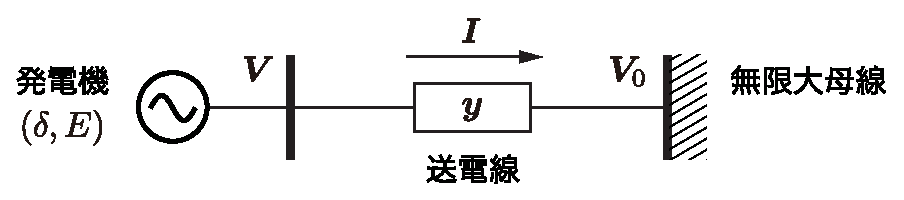
\includegraphics[width = .70\linewidth]{figs/inf1bus}
\medskip
\caption{\textbf{1 infinity bus system model}}
\label{fig:inf1bus}
\medskip
\end{figure}

In basic mathematical analysis in electrical power system engineering, for example, a simplified electrical power system model, called a \textbf{single machine infinite bus system model}, such as \cite[Section 1.3]{taniguchi2011power} and \cite[Section 6.3, Section 8.3]{kato2017electric}, is often used. 
The single machine infinite bus system model is an electrical power system model consisting of a generator, transmission line, and infinite bus bar as shown in \ref{fig:inf1bus}.
The infinite bus bar is interpreted as a rough approximation of the entire electrical power system, except for the generator of interest, as a “fixed voltage source.”

%\footnote{
%ここでの「電力系統全体」には, その他の発電機や負荷, 送電網などのすべての構成要素が含まれる。
%1機無限大母線系統モデルでは, それらすべてをまとめて固定された電圧源とみなしてしまう。
%}。
Specifically, we assume that voltage phasor of the infinite bus bar $\bm{V}_0$ is maintained as a constant, independent of the internal state of the generator.
In other words, considering electric power that is lost in transmission, the active and reactive power generated by the generator are assumed to be consumed each moment, without excess or deficiency, by the infinite bus bar.



As follows, since there is only one generator of interest, we omit the subscript $i$, and note the variables of the generator and generator bus.
For the dynamic characteristics of the generator expressed in Equation (\ref{eq:gendynVI}), the voltage phasor $\bm{V}$ and current phasor $\bm{I}$ of a generator bus have the following relationship:
\[
\bm{I}= \bm{y} (\bm{V}-\bm{V}_0)
%\qquad
%\Longleftrightarrow
%\qquad
%\bm{V} = \tfrac{1}{\bm{y}} \bm{I} +\bm{V}_0
\]
This is the algebraic equation that determines the input-output relationship of the generator and the electrical power system. 
For reference, let us derive an ordinary differential equation model obtained through Kron reduction for a single machine infinite bus bar system when the resistance of a transmission line is 0, and the reactance is $x$; in other words, the admittance of a transmission line is:
\[
\bm{y} = \frac{1}{\bm{j} x}
\]
Specifically, using the same procedure as that used for Kron reduction of a generator bus in Section \ref{sec:allgen}, 
the following two equations are used:
\[
\bm{I}= \frac{1}{\bm{j} x} (\bm{V}-\bm{V}_0)
,\qquad
\bm{I}= \frac{1}{\bm{j} \Xt} (Ee^{\bm{j}\delta} -\bm{V})
\]
to cancel the current phasor and voltage phasor of the generator bus.
When the voltage phasor is cancelled and the Equation is reorganized, the following is obtained:
\[
|\bm{I}| e^{\bm{j}(\delta -\angle \bm{I})}
=
-\frac{
E- |\bm{V}_0|e^{\bm{j}\delta}
}{
\bm{j}(\Xt + x )
}
\]
It is assumed that $\angle \bm{V}$ is 0 with the phase of voltage phasor of the infinite bus bar as the reference, and generality is not lost.
Therefore, by substituting the relationship of this current phasor into Equation \ref{eq:gendynIVst}, the expression of the ordinary differential equation system is obtained as follows:
\begin{align*}%\label{eq:gendynIVst}
\simode{
\dot{\delta} &= \omega_0  \Delta \omega\\
M   \Delta \dot{\omega}&= \textstyle
 - D \Delta\omega  - 
\tfrac{
E|\bm{V}_0|
}{
\Xt + x
}
\sfsin\delta
+P_{{\rm mech}}
\\
\taud \dot{E} & = \textstyle
 - 
 \tfrac{
\Xs + x
}{
\Xt + x
}
E
+
\tfrac{
\Xs - \Xt
}{
\Xt + x
}
|\bm{V}_0| \sfcos\delta
+ V_{{\rm field}}
}
\end{align*}
Similarly, the active and reactive power supplied from the generator to the generator bus are obtained as follows from the relationship of Equation \ref{eq:PiQis2}:
\[
P=\frac{
E|\bm{V}_0|\sfsin\delta
}{
\Xt + x
}
,\qquad
Q=
\frac{
x E^2 + (\Xt - x )E|\bm{V}_0|\sfcos\delta
- \Xt |\bm{V}_0|^2
}{
( \Xt + x )^2
}
\]
As a reference, we introduced the single machine infinite bus system model, but since we focus on an analysis of an electrical power system model consisting of multiple generators in this book, analysis with this model is basically not performed.


\subsection{Mathematical properties of the admittance matrix with reduced generator bus}

Below, we mathematically discuss the existence and definiteness of the reduced admittance matrix $\bm{Y}^{\rm red}$ of Equation \ref{eq:Yred}.
Let us remember that with the admittance matrix $\bm{Y}_0$ when the capacitance to ground of Equation (\ref{eq:Y0prop}) can be ignored, the real part of the conductance matrix $G_0$ is positive semi-definite and the imaginary part of the susceptance matrix $B_0$ is negative definite.
The reduced admittance matrix also has a similar definiteness.
Below, the reduced conductance matrix and reduced susceptance matrix, the real and imaginary parts of $\bm{Y}^{\rm red}$, are expressed as follows:
\begin{align}\label{eq:GredBred}
G^{\rm red} :=\real\bigl[\bm{Y}^{\rm red}\bigr] ,\qquad
B^{\rm red} :=\imag\bigl[\bm{Y}^{\rm red}\bigr] 
\end{align}

At this time, the following facts are indicated.


\begin{theorem}[existence and definiteness of the reduced admittance matrix]
\label{thm:redadmat}
If the following is true for the admittance matrix $\bm{Y}\in \mathbb{C}^{N\times N}$ of Equation \ref{eq:Ypig}:
\begin{align}\label{eq:Xbeta}
\Cgi \Xti \leq 1
,\qquad \forall i \in \mathcal{I}_G
\end{align}
And the inequality holds exactly for Equation \ref{eq:Xbeta} for at least one generator bus at the same time, $\bm{\itGamma}$ of Equation \ref{eq:defGam} is nonsingular.
At this time, for the admittance matrix $\bm{Y}^{\rm red}$ of Equation \ref{eq:Yred}, the reduced conductance matrix $G^{\rm red}$ is positive semi-definite, and the reduced susceptance matrix $B^{\rm red}$ is negative definite.
\end{theorem}

\begin{proof}
\red{Translated with DeepL}
By using the complementary ref{lem:nonsing} at the end of the chapter, we show the regularity of $\bm{\itGamma}$ in the formula\ref{eq:defGam}.
From the definition, if the real part of $\bm{\itGamma}$ is $M$ and the imaginary part is $N$, then
\begin{align*}
\spliteq{
M &:= \sfdiag \bigl( \Xti (1- \Cgi \Xti ) \bigr) 
- \sfdiag \left( \Xti \right) B_0 \sfdiag \left( \Xti \right), \\
N &:= - \sfdiag \left( \Xti \right) G_0 \sfdiag \left( \Xti \right)
}
\end{align*}
Here, since $B_0$ in equation\ref{eq:Ypig} is semi-negative definite, $M$ is at least semi-positive definite when equation\ref{eq:Xbeta} holds.
If $\Cgi \Xti <1$ for at least one $i\in \mathcal{I}_G$, then
\begin{align*}
\underbrace{
\sfker \sfdiag \left( \Xti \right) B_0 \sfdiag \left( \Xti \right)
}_{\sfspan \left\{ \sfdiag \left( 1/\Xti \right) \mathds{1} \right\}}
\nsubseteq
\sfker \sfdiag \bigl( \Xti (1- \Cgi \Xti ) \bigr)
\end{align*}
then, $M$ is positive definite.
Therefore, since $N$ is symmetric, $M+NM^{-1}N$ is positive definite. This implies that $M+NM^{-1}N$ is regular.
Also, since $N$ is semi-negative definite from the relation in equation\ref{eq:Y0}, from the complement\ref{lem:sdreim} at the end of the chapter,
it can be shown that the real part of $\bm{\itGamma}^{-1}$ is positive definite and the imaginary part is semi-negative definite.
Therefore, the real part $G^{\rm red}$ of $\bm{Y}^{\rm red}$ is semipositive definite and the imaginary part $B^{\rm red}$ is negative definite.
\end{proof}

Inequality in Equation \ref{eq:Xbeta} is the condition required for $\bm{\itGamma}$ to be nonsingular. 
However, if $ \Cgi \Xti $ is 1 for all generator buses, $\bm{\itGamma}$ is no longer nonsingular.
If all $\Cgi$ is sufficiently small; in other words, if the capacitance to ground of each transmission line can be ignored as in the Example \ref{ex:derY}, inequality of Equation \ref{eq:Xbeta} holds.
At this time, the reduced conductance matrix $G^{\rm red}$, the real part of $\bm{Y}^{\rm red}$, is positive semi-definite. The imaginary part, the reduced susceptance matrix $B^{\rm red}$, is negative definite.
For this reason, the definiteness of the admittance matrix is invariable to the Kron reduction.


\subsection{Mathematical model for salient pole synchronous generators}\label{sec:genmodadv}

Let us look at a salient pole generator model that incorporates the difference in the reactance of the d-axis and q-axis.
Specifically, let us consider a situation where Equation \ref{eq:phVIsincos} is as follows:
\begin{align}\label{eq:phVIsincosC_}
\spliteq{
|\bm{V}_i| \sfsin (\delta_i -\angle \bm{V}_i)  &= 
X_{{\rm q}i} |\bm{I}_i| \sfcos (\delta_i -\angle \bm{I}_i),\\
|\bm{V}_i| \sfcos (\delta_i -\angle \bm{V}_i)  & = E_i - 
X_{{\rm d}i}' |\bm{I}_i| \sfsin (\delta_i -\angle \bm{I}_i)
}
\end{align}
$X_{{\rm d}i}'$ is the transient reactance of the d-axis.
If $X_{{\rm d}i}'$ and $X_{{\rm q}i}$ are equal $\Xti$, Equation \ref{eq:phVIsincosC_} is consistent with Equation \ref{eq:phVIsincos}.

When cancelling the current phasor using Equation \ref{eq:phVIsincosC_}, the active and reactive power are expressed as:
\begin{align}\label{eq:PQV_}
\spliteq{
P_i &=  \frac{|\bm{V}_i | E_i}{X_{{\rm d}i}'} \sfsin(\delta_i -  \angle \bm{V}_i) \\
  & \hspace{2em}-  
\left( \frac{1}{X_{{\rm d}i}'}  -  \frac{1}{X_{{\rm q}i}} \right)
|\bm{V}_i|^2 \sfsin( \delta_i - \angle \bm{V}_i)\sfcos( \delta_i - \angle \bm{V}_i), \\
Q_i &=  \frac{|\bm{V}_i|E_i}{X_{{\rm d}i}'} \sfcos (\delta_i - \angle \bm{V}_i) \\
 & \hspace{2em} -|\bm{V}_i|^2 \left( \frac{\sfcos^2 (\delta_i - \angle \bm{V}_i) }{X_{{\rm d}i}'} 
+ \frac{\sfsin^2 (\delta_i - \angle \bm{V}_i)}{X_{{\rm q}i}} \right)
}
\end{align}
Similarly, if the voltage phasor is cancelled, the following is obtained:
\begin{align}\label{eq:PQI}
\spliteq{
P_i &=  E_i |\bm{I}|  \sfcos(\delta_i -  \angle \bm{I}_i) \\
 & \hspace{2em} - (X_{{\rm d}i}' -X_{{\rm q}i}) |\bm{I}_i|^2  \sfsin(\delta_i -  \angle \bm{I}_i)\sfcos(\delta_i -  \angle \bm{I}_i), \\
Q_i &= E_i |\bm{I}_i| \sfsin (\delta_i - \angle \bm{I}_i)  \\
 & \hspace{2em}- |\bm{I}_i|^2 \left\{
X_{{\rm d}i}'  \sfsin^2  (\delta_i - \angle \bm{I}_i) 
+ X_{{\rm q}i} \sfcos^2  (\delta_i - \angle \bm{I}_i)  
\right\}
}
\end{align}

The oscillation equation and dynamic characteristics of generators combined with magnetic flux attenuation are given with the following in the same manner as Equation (\ref{eq:gendynVI}):
\begin{subequations}\label{eq:gendynVI_}
\begin{align}\label{eq:gendynVIst_}
\simode{
\dot{\delta}_i&= \omega_0  \Delta \omega_i\\
M_i   \Delta \dot{\omega}_i&= 
 - D_i \Delta\omega_i  
 - P_i 
+P_{{\rm mech}i} 
\\
\taudi \dot{E}_i & = 
 -\tfrac{X_{{\rm d}i}}{X_{{\rm d}i}'}E_i
+\left(
\tfrac{X_{{\rm d}i}}{X_{{\rm d}i}'}-1
\right)
|\bm{V}_i| \sfcos (\delta_i - \angle \bm{V}_i ) 
+ V_{{\rm field}i}
}
\end{align}
However, for active power $P_i$, the expression of Equation \ref{eq:PQV_} is used.
Here, the voltage phasor is considered an input from the electrical power system to the generator $i$.
In addition, the current phasor becomes an output from the generator to the electrical power system:

\begin{align}\label{eq:Iout_}
\spliteq{
|\bm{I}_i| &= \textstyle \sqrt{
\left\{ \tfrac{|\bm{V}_i|}{X_{{\rm q}i}} \sfsin(\delta_i - \angle \bm{V}_i) \right\}^2
+\left\{ \tfrac{E_i}{X_{{\rm d}i}'} - \tfrac{|\bm{V}_i|}{X_{{\rm d}i}'} \sfcos(\delta_i - \angle \bm{V}_i) \right\}^2
}, \\
\angle \bm{I}_i &= %\textstyle 
\delta_i - \sfarctan \left(
\frac{\tfrac{E_i}{X_{{\rm d}i}'} - \tfrac{|\bm{V}_i|}{X_{{\rm d}i}'} \sfcos(\delta_i - \angle \bm{V}_i)}{
\tfrac{|\bm{V}_i|}{X_{{\rm q}i}} \sfsin(\delta_i - \angle \bm{V}_i)
}
\right)
}
\end{align}
\end{subequations}
This is derived from Equation \ref{eq:phVIsincosC_}.
\begin{subequations}\label{eq:gendynIV_}
Similarly, if current phasor is considered as an input from the electrical power system to the generator $i$, the following becomes the equation of state that expresses the dynamic characteristics of the generator:
\begin{align}\label{eq:gendynIVst_}
\simode{
\dot{\delta}_i &= \omega_0  \Delta \omega_i\\
M_i   \Delta \dot{\omega}_i&= \textstyle
 - D_i \Delta\omega_i  - 
P_i
+P_{{\rm mech}i}
\\
\taudi \dot{E}_i & = \textstyle
 - E_i
-(
X_{{\rm d}i} - X_{{\rm d}i}'
)
|\bm{I}_i| \sfsin (\delta_i - \angle \bm{I}_i ) 
+ V_{{\rm field}i}
}
\end{align}
For active power $P_i$, the expression of Equation \ref{eq:PQI} is used.
The voltage phasor obtained from: 
\begin{align}\label{eq:Vout_}
\spliteq{
|\bm{V}_i| &= \textstyle \sqrt{
\bigl\{ X_{{\rm q}i} |\bm{I}_i| \sfcos(\delta_i - \angle \bm{I}_i) \bigr\}^2
+\left\{ E_i - X_{{\rm d}i}' |\bm{I}_i| \sfsin(\delta_i - \angle \bm{I}_i) \right\}^2
}, \\
\angle \bm{V}_i &= %\textstyle 
\delta_i - \sfarctan \left(
\frac{
X_{{\rm q}i} |\bm{I}_i| \sfcos(\delta_i - \angle \bm{I}_i)
}
{
E_i - X_{{\rm d}i}' |\bm{I}_i| \sfsin(\delta_i - \angle \bm{I}_i)
}
\right)
}
\end{align}
which is derived from Equation \ref{eq:phVIsincosC_}, is an output from the generator to the electrical power system. 
\end{subequations}
This salient pole generators model assumes that $X_{{\rm d}i}'$ and $X_{{\rm q}i}$ are equal and $\Xti$, and if $X_{{\rm d}i}$ is substituted with $\Xsi$, it becomes consistent with the generator model discussed in Section \ref{sec:genfund}.
The relationship, $X_{{\rm d}i}>X_{{\rm q}i}> X_{{\rm d}i}'$ usually holds between these reactances.

\begin{COLUMN}
\red{Translated with DeepL}
\noindent \textbf{Relationship between generator models}:
The relationship between the 2-axis model, 1-axis model, and classical model can be understood as the difference in the magnitude of the time constant in the dynamic characteristics of magnetic flux attenuation.
The equation of state of the 2-axis model when the voltage phasor of the bus is regarded as the input is
\begin{equation*}
  \begin{aligned}%\label{eq:gendyn2a}
    \begin{cases}
      \dot{\delta}_i&= \omega_0  \Delta \omega_i\\
      M_i   \Delta \dot{\omega}_i&= 
      - D_i \Delta\omega_i  
      - P_i 
      +P_{{\rm mech}i} 
      \\
      \tau_{{\rm d}i} \dot{E}_{{\rm q}i} & = 
      - \tfrac{ X_{{\rm d}i} }{ X_{{\rm d}i}' }E_{{\rm q}i}
      +\left(
      \tfrac{ X_{{\rm d}i} }{ X_{{\rm d}i}' } -1
      \right)
      \bm{V}_{{\rm q}i}
      + V_{{\rm field}i} \\
      \tau_{{\rm q}i} \dot{E}_{{\rm d}i} & = 
      - \tfrac{ X_{{\rm q}i} }{ X_{{\rm q}i}' }E_{{\rm d}i}
      +\left(
      \tfrac{ X_{{\rm q}i} }{ X_{{\rm q}i}' } -1
      \right)
      \bm{V}_{{\rm d}i}
    \end{cases}
  \end{aligned}
\end{equation*}
However, $X_{{\rm q}i}'$ is the transient reactance of the q axis.
\[
\bm{V}_{{\rm d}i}:=
|\bm{V}_i| \sfsin (\delta_i - \angle \bm{V}_i ) 
,\qquad
\bm{V}_{{\rm q}i}:=
|\bm{V}_i| \sfcos (\delta_i - \angle \bm{V}_i ) 
\]
Also, the output equations for active power and reactive power are:
\begin{equation*}
  \begin{aligned}%\label{eq:gendyn2ao}
    \begin{cases}
      P_i & =  \frac{E_{{\rm q}i}}{X_{{\rm d}i}' } \bm{V}_{{\rm d}i}
      - \frac{E_{{\rm d}i}}{X_{{\rm q}i}' } \bm{V}_{{\rm q}i}
      +
      \left(
      \frac{1}{X_{{\rm q}i}'} - \frac{1}{X_{{\rm d}i}'} 
      \right)
      \bm{V}_{{\rm d}i} \bm{V}_{{\rm q}i}
      , \\
      Q_i & =  
      \frac{E_{{\rm q}i}}{X_{{\rm d}i}' } \bm{V}_{{\rm q}i}
      + \frac{E_{{\rm d}i}}{X_{{\rm q}i}' } \bm{V}_{{\rm d}i}
      -
      \left(
      \frac{\bm{V}_{{\rm d}i}^2}{X_{{\rm q}i}'} 
      +
      \frac{\bm{V}_{{\rm q}i}^2 }{X_{{\rm d}i}'} 
      \right)
    \end{cases}
  \end{aligned}
\end{equation*}
Note that the state variables of the internal voltage have increased to two, $E_{{\rm d}i}$ and $E_{{\rm q}i}$.
This two-axis model is known to match the salient pole-type one-axis model in the limit when the time constant $\tau_{{\rm q}i}$ is small enough.
Specifically, assuming that $\tau_{{\rm q}i}$ is formally 0, the state variable $E_{{\rm d}i}$ satisfies the following relationship over time.
\[
0=- \frac{ X_{{\rm q}i} }{ X_{{\rm q}i}' }E_{{\rm d}i}
+\left(
\frac{ X_{{\rm q}i} }{ X_{{\rm q}i}' } -1
\right)
\bm{V}_{{\rm d}i}
\]
At this time, the active power and the active power are
\begin{equation*}
  \begin{aligned}
    \begin{cases}
      P_i & =  \frac{E_{{\rm q}i}}{X_{{\rm d}i}' } \bm{V}_{{\rm d}i}
      +
      \left(
      \frac{1}{X_{{\rm q}i} } - \frac{1}{X_{{\rm d}i}'} 
      \right)
      \bm{V}_{{\rm d}i} \bm{V}_{{\rm q}i}
      , \\
      Q_i & =  
      \frac{E_{{\rm q}i}}{X_{{\rm d}i}' } \bm{V}_{{\rm q}i}
      -
      \left(
      \frac{\bm{V}_{{\rm d}i}^2}{X_{{\rm q}i} } 
      +
      \frac{\bm{V}_{{\rm q}i}^2 }{X_{{\rm d}i}'} 
      \right)
    \end{cases}
  \end{aligned}
\end{equation*}
That is, the dynamic characteristics of the generator model match those of the salient pole type uniaxial model.
Furthermore, in the limit when the time constant $\tau_{{\rm d}i}$ is also small enough
\begin{equation*}
  \begin{aligned}
    \begin{cases}
      P_i & =  \frac{V_{{\rm field}i}}{X_{{\rm d}i} } \bm{V}_{{\rm d}i}
      +
      \left(
      \frac{1}{X_{{\rm q}i} } - \frac{1}{X_{{\rm d}i} } 
      \right)
      \bm{V}_{{\rm d}i} \bm{V}_{{\rm q}i}
      , \\
      Q_i & =  
      \frac{V_{{\rm field}i}}{X_{{\rm d}i} } \bm{V}_{{\rm q}i}
      -
      \left(
      \frac{\bm{V}_{{\rm d}i}^2}{X_{{\rm q}i} } 
      +
      \frac{\bm{V}_{{\rm q}i}^2 }{X_{{\rm d}i} } 
      \right)
    \end{cases}
  \end{aligned}
\end{equation*}
In particular, it is non-polar, that is, $X_{{\rm d}i}$ and $X_{{\rm q}i}$ are equal $X_i$, and the field input.
Assuming that $V_{{\rm field}i}$ is constant with the constant $V_{i}^{\star}$:
\[
P_i = \frac{V_{i}^{\star} |\bm{V}_i| }{X_i } \sfsin (\delta_i - \angle \bm{V}_i ) 
,\qquad
Q_i = \frac{V_{i}^{\star} |\bm{V}_i| }{X_i }  \sfcos (\delta_i - \angle \bm{V}_i ) 
- \frac{|\bm{V}_i|^2 }{X_i }
\]
This matches the classic model.
For the detailed derivation process, refer to \cite[Section 5]{sauer2017power}.
\end{COLUMN}



\section{Mathematical model of load}\label{sec:modload}

\subsection{Relational expression of current and voltage based on load characteristics}\label{sec:loadpr}

\begin{figure}[t]
\centering
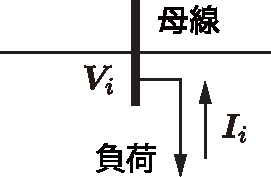
\includegraphics[width = .25\linewidth]{figs/loadbus}
\medskip
\caption{\textbf{Load connected to bus bar}}
\label{fig:loadbus}
\medskip
\end{figure}

As a static load model, three types of models — \textbf{constant impedance model}, \textbf{constant power model}, and \textbf{constant current model}— or their combinations are often used.
These are all static models described by algebraic equations related to the current phasor and voltage phasor. 
Let us assume that voltage phasor of a bus bar $i$ connected with a load is $\bm{V}_i$ and the current phase flowing from the load to the bus bar is $\bm{I}_i$ (\ref{fig:loadbus}).
At this time, the constant impedance model gives the following relationship:
\begin{subequations}\label{eq:ldynVI}
\begin{align}\label{eq:cimp}
\bm{I}_i= - \frac{ \bm{V}_i}{\bm{z}_{{\rm load}i}^{\star}}
\end{align}
where, $\bm{z}_{{\rm load}i}^{\star} \in \mathbb{C}$ is a constant that expresses the impedance of the load.
Here, the reason that there is a negative sign on the right side of Equation \ref{eq:cimp} is that the equipment that is equivalent to the load is grounded, and the direction of the flow from the load to the bus bar $i$ is defined as positive sign of the current phasor $\bm{I}_i$.
Specifically:
\[
\bm{I}_i= \frac{1}{\bm{z}_{{\rm load}i}^{\star}} (0-\bm{V}_i)
\]
Incandescent lamps and electric heaters are expressed as the constant impedance model.

The constant current model gives the following relationship with the constant that represents the fixed current phasor as $\bm{I}_{{\rm load}i}^{\star} \in \mathbb{C}$:
\begin{align}\label{eq:ccrt}
\bm{I}_i = \bm{I}_{{\rm load}i}^{\star} e^{\bm{j} \angle \bm{V}_i }
\end{align}
In other words, the following is true for the absolute value $|\bm{I}_{{\rm load}i}^{\star}|$ and phase $\angle \bm{I}_{{\rm load}i}^{\star}$:
\[
|\bm{I}_i| = |\bm{I}_{{\rm load}i}^{\star}|,\qquad
\angle \bm{I}_i = \angle \bm{I}_{{\rm load}i}^{\star} + \angle \bm{V}_i
\]
The constant power model gives the following relationship:
\begin{align}\label{eq:cpw}
\bm{I}_i = \frac{P_{{\rm load}i}^{\star} - \bm{j} Q_{{\rm load}i}^{\star} }{\overline{\bm{V}}_i}
\end{align}
\end{subequations}
where $P_{{\rm load}i}^{\star} \in \mathbb{R}$ and $Q_{{\rm load}i}^{\star} \in \mathbb{R}$ are constants that express the active and reactive power supplied to the bus bar $i$.
This is derived by considering the complex conjugate of:
\[
P_{{\rm load}i}^{\star} + \bm{j} Q_{{\rm load}i}^{\star} =
\bm{V}_i \overline{\bm{I}}_i
\]
The electric power converter is expressed as the constant current model and the constant power model based on its properties.

Depending on the purpose of the analysis, a dynamic load model might be employed.
Please see \cite[Section 7.1.2]{kundur1994power} for further details.


\subsection{Kron reduction of the load bus bar}

When there are generators and multiple types of loads, the relationship between the current phasor and voltage phasor of each device is stipulated by Equations (\ref{eq:gendynVI}) and (\ref{eq:ldynVI}), and by combining these with Equation \ref{eq:ohmY}, the mathematical model of the entire electrical power system can be obtained.
At this time, the constant impedance model of Equation \ref{eq:cimp} provides a linear relationship for the current phasor and voltage phasor.
On the other hand, since the constant current model of Equation \ref{eq:ccrt} and the constant power model of Equation \ref{eq:cpw} give a nonlinear relationship for the current phasor and voltage phasor, mathematical analysis of the obtained electrical power system model would generally be difficult.
Let us confirm with the following example.

\begin{example}{Kron reduction of load bus bar}\label{ex:genloadY}
Let us assume that in the electrical power system of the Example \ref{ex:derY}, the generators are connected as equipment 1 and equipment 2, and load is connected as equipment 3.
The relationship of the current phasor vector and voltage phasor vector of the admittance matrix of a power grid is given by Equation \ref{eq:exY}.
First, let us consider a case where the load is given as the constant impedance model.
If $\bm{z}_{{\rm load}3}^{\star}$ is the impedance of the load, the following Equation is obtained:
\[
\bm{I}_3 = -\frac{ \bm{V}_3}{\bm{z}_{{\rm load}3}^{\star}}
\]
If this is substituted into Equation \ref{eq:exY} to cancel $\bm{I}_3$, the following is obtained:
\begin{align}\label{eq:exYcimp}
\mat{
\bm{I}_1\\
\bm{I}_2\\
0\\
}
=
\mat{
\bm{y}_{12} & -\bm{y}_{12} & 0\\
-\bm{y}_{12} & \bm{y}_{12}+\bm{y}_{32} & -\bm{y}_{32}\\
0 & -\bm{y}_{32} & \bm{y}_{32}  + \tfrac{1}{\bm{z}_{{\rm load}3}^{\star}}
}
\mat{
\bm{V}_1\\
\bm{V}_2\\
\bm{V}_3\\
}
\end{align}
Please note that, with the Equation on the third row, voltage phasor $\bm{V}_3$ of the load bus bar is replaced by voltage phasor $\bm{V}_2$ of the generator bus.
Specifically, it can be expressed as:
\begin{align*}
\bm{V}_3 = \left(\bm{y}_{32} + \tfrac{1}{\bm{z}_{{\rm load}3}^{\star}} \right)^{-1} \bm{y}_{32} \bm{V}_2
\end{align*}

If we also eliminate $\bm{V}_3$ using this, the relationship between the current and voltage phasors of the generator bus bar group is
\begin{align*}
\mat{
\bm{I}_1\\
\bm{I}_2
}
=
\bm{Y}_{\rm Kron}
\mat{
\bm{V}_1\\
\bm{V}_2\\
}
\end{align*}
Here, the reduced admittance matrix of the load bus bar is obtained as:
\[
\bm{Y}_{\rm Kron}:=
\mat{
\bm{y}_{12} & -\bm{y}_{12}\\
-\bm{y}_{12} & \bm{y}_{12}+\bm{y}_{32}
}
-
\mat{
0\\
\bm{y}_{32}
}
\left( 
\bm{y}_{32} 
+ \tfrac{1}{\bm{z}_{{\rm load}3}^{\star}} 
\right)^{-1}
\mat{
0&\bm{y}_{32}
}
\]
Therefore, if the load is given as the constant impedance model, $\bm{Y}_{\rm Kron} \in \mathbb{C}^{2\times 2}$ obtained in this way 
is considered as the admittance matrix of a new power grid to cancel the load bus bar and its variable, allowing for equivalent transformation to a differential-algebraic equation system where only generators are connected to bus bars. 

Next, let us consider a situation where the load is given as the constant current model.
Let us assume that current phasor flows from the load to bus bar 3:
\[
\bm{I}_3 = \bm{I}_{{\rm load}3}^{\star} e^{\bm{j} \angle \bm{V}_3}
\]
At this time, in the same procedure as the constant impedance model, if $\bm{I}_3$ and $\bm{V}_3$ 
are cancelled from Equation \ref{eq:exY}, the following is obtained:
\begin{align*}
\mat{
\bm{I}_1\\
\bm{I}_2
}
=
\bm{Y}_{\rm Kron}'
\mat{
\bm{V}_1\\
\bm{V}_2\\
}
+
\mat{
0\\
-\bm{y}_{32}
}
\bm{y}_{32}^{-1}
\bm{I}_{{\rm load}3}^{\star} e^{\bm{j} \angle \bm{V}_3}
\end{align*}
where:
\[
\bm{Y}_{\rm Kron}' :=
\mat{
\bm{y}_{12} & -\bm{y}_{12}\\
-\bm{y}_{12} & \bm{y}_{12}+\bm{y}_{32}
}
-
\mat{
0\\
\bm{y}_{32}
}
\bm{y}_{32}^{-1}
\mat{
0&\bm{y}_{32}
}
\]
This means that, if the load is given as the constant current model, an affine relationship is given to the current phasor and voltage phasor of the generators.
However, phase $\angle \bm{V}_3$ of the voltage phasor of the load bus bar also has an impact on the current phasor of the generators.
Generally, phase $\angle \bm{V}_3$ of the voltage phasor is a nonlinear function of the voltage phasor $\bm{V}_3$.


Finally, let us consider a case wherein the load is given as the constant power model.
When a constant active power $P_{{\rm load}3}^{\star}$ and reactive power $Q_{{\rm load}3}^{\star}$ are supplied from the load to bus bar 3, the following relationship is given:
\begin{align*}
\bm{I}_3 = \frac{P_{{\rm load}3}^{\star} - \bm{j} Q_{{\rm load}3}^{\star} }{\overline{\bm{V}}_3}
\end{align*}
Since this is a nonlinear relationship of $\bm{I}_3$ and $\bm{V}_3$, to cancel $\bm{V}_3$ from Equation \ref{eq:exY}, nonlinear calculation is necessary.
Specifically, $\bm{V}_3$ is given as a solution for the quadratic equation related to complex variables:
\begin{align*}
\bm{y}_{32} \bm{V}_3 \overline{\bm{V}}_3 - \bm{y}_{32}  \bm{V}_2 \overline{\bm{V}}_3 -P_{{\rm load}3}^{\star} 
+ \bm{j} Q_{{\rm load}3}^{\star} =0
\end{align*}
Therefore, if the load of the constant power model is included in an electrical power system model, it is usually difficult to cancel the load bus bar through equivalent transformation.
\end{example}

As shown in Example \ref{ex:genloadY}, if the load is given as a static model expressed by Equation (\ref{eq:ldynVI}), the current phasor and voltage phasor of some or all load bus bars can be equivalently cancelled through algebraic calculation.
This operation is called \textbf{Kron reduction of the load bus bar}.
Specifically, when the load is given as the constant impedance model, Kron reduction of the load bus bar corresponds to reducing the dimension of the admittance matrix of the power grid by mathematically equivalent calculation.

If there is no equipment, such as a generator or load, connected to the bus bar, we can assume that the absolute value of $\bm{z}_{{\rm load}i}^{\star}$ in Equation \ref{eq:cimp} is where the load of an infinite constant impedance model is connected to the bus bar $i$.
This is equal to virtually connecting the load of the constant current model, where the current phasor between the load and the bus bar is always 0.
Therefore, the above-described Kron reduction of the load bus bar allows for equivalent cancellation of the bus bar without equipment.


\subsection{Mathematical properties of the admittance matrix with reduced load bus bar}

Let us analyze properties that hold for Kron reduction of the load bus bar when all loads are given by the constant impedance model.
First, we will show Kron reduction steps for the Example \ref{ex:genloadY} as a general form when generator buses and load bus bars are arbitrary.
The subscripts set of generator buses is $\mathcal{I}_{\rm G}$ and the subscripts set of load bus bars is $\mathcal{I}_{\rm L}$.
We assume that a smaller number is assigned to general buses than load bus bars without losing generality. In other words:
\begin{align*}
\mathcal{I}_{\rm G} = \{ 1,\ldots, n \},\qquad
\mathcal{I}_{\rm L} = \{ n+1,\ldots, n + m \}
\end{align*}
where $n$ and $m$ are numbers of generator buses and load bus bars, respectively.
The definition stipulates that $n+m$ is equal to the total number of bus bars $N$.

A vector with current phasors of all generator buses is $\bm{I}_{\rm G} \in \mathbb{C}^{n}$ and a vector with voltage phasors of all generator buses is $\bm{V}_{\rm G} \in \mathbb{C}^{n}$.
Similarly, a vector with current phasors of all load bus bars is $\bm{I}_{\rm L}\in \mathbb{C}^{m}$ and a vector of voltage phasors of all load bus bars is $\bm{V}_{\rm L} \in \mathbb{C}^{m}$.
At this time, the relationship between all current phasors and voltage phasors related to the admittance matrix of power grids $\bm{Y}\in \mathbb{C}^{N\times N}$ can be expressed as:
\begin{align}\label{eq:YGL}
\mat{
\bm{I}_{\rm G}\\
\bm{I}_{\rm L}
}
=
\underbrace{
\mat{
\bm{Y}_{\rm GG} & \bm{Y}_{\rm GL}\\
\bm{Y}_{\rm LG} & \bm{Y}_{\rm LL}
}
}_{\bm{Y}}
\mat{
\bm{V}_{\rm G}\\
\bm{V}_{\rm L}
}
\end{align}
The relationship between the current phasor and voltage phasor determined by the load of the constant impedance model can be expressed as follows by using the admittance, which is a reciprocal of the impedance:
\begin{align*}
\bm{I}_{\rm L}=- \sfdiag(\bm{y}_{{\rm load}i}^{\star} )_{i \in \mathcal{I}_{\rm L}}\bm{V}_{\rm L}
\end{align*}
Though $\bm{y}_{{\rm load}i}^{\star}$ defined as a reciprocal of $\bm{z}_{{\rm load}i}^{\star}$ of Equation \ref{eq:cimp} must have a non-zero value, since this is an expression of bus bars with no equipment connected, formally, $\bm{y}_{{\rm load}i}^{\star}$ is allowed to be 0.
If this is substituted into Equation \ref{eq:YGL} to cancel $\bm{V}_{\rm L}$:
\begin{align}\label{eq:Kron}
\bm{I}_{\rm G} = 
\Bigl\{ 
\underbrace{
\bm{Y}_{\rm GG} - \bm{Y}_{\rm GL} 
\bigl( \bm{Y}_{\rm LL} + \sfdiag(\bm{y}_{{\rm load}i}^{\star} )_{i \in \mathcal{I}_{\rm L}} \bigr)^{-1}
\bm{Y}_{\rm LG} 
}_{\bm{Y}_{\rm Kron}}
\Bigr\}
\bm{V}_{\rm G}
\end{align}
is obtained.
Note that, generally, when a load consumes active power and reactive power in terms of the admittances of the load, similar to a transmission line, the following is established: 
\begin{align}\label{eq:loadys}
\real[\bm{y}_{{\rm load}i}^{\star} ] \geq 0 ,\qquad
\imag[\bm{y}_{{\rm load}i}^{\star} ] \leq 0
,\qquad
\forall i \in \mathcal{I}_{\rm L}
\end{align}
The conductance and susceptance matrices, where the load bus bar, which is the real and imaginary part of $\bm{Y}_{\rm Kron}$, is reduced, are expressed as:
\[
G_{\rm Kron} := \real \bigl[  \bm{Y}_{\rm Kron}  \bigr] ,\qquad
B_{\rm Kron} := \imag \bigl[  \bm{Y}_{\rm Kron}  \bigr]
\]
This presents the following fact:

\begin{theorem}[Properties of the Kron-reduced admittance matrix]
\label{thm:Kron}
For the admittance matrix $\bm{Y}\in \mathbb{C}^{N\times N}$ of Equation \ref{eq:Ypig}, 
the partitioned matrix of Equation \ref{eq:YGL} defines the admittance matrix where the load bus bars have been Kron reduced as 
$\bm{Y}_{\rm Kron}\in \ \mathbb{C}^{n\times n}$ of Equation \ref{eq:Kron}. 
The admittance $\bm{y}_{{\rm load}i}^{\star} $ of each load satisfies Equation \ref{eq:loadys}. 
At this point, the reduced conductance matrix $G_{\rm Kron}$ is positive semi-definite, while the reduced susceptance matrix 
$B_{\rm Kron}$ is symmetric. If the following is true for generator buses:
\begin{subequations}\label{eq:betas}
\begin{align}\label{eq:betag}
\Cgi = 0
,\qquad
\forall i \in \mathcal{I}_{\rm G}
\end{align}
And the following is true for load bus bars:
\begin{align}\label{eq:betay}
\imag[\bm{y}_{{\rm load}i}^{\star} ] + \Cgi \leq 0
,\qquad
\forall i \in \mathcal{I}_{\rm L}
\end{align}
\end{subequations}
$B_{\rm Kron}$ is negative semi-definite.
where $\Cgi$ is a non-negative constant equivalent to the capacitance to ground of Equation \ref{eq:Ypig}. 
Specifically, if the inequality of Equation \ref{eq:betay} strictly holds for at least one load bus bar, 
$B_{\rm Kron}$ is negative definite.
\end{theorem}

\begin{proof}

\red{Translated with DeepL}
To show the subject using the Lemma \ref{lem: schur} at the end of the chapter
\begin{align*}
\bm{Y}' := 
\mat{
\bm{Y}_{\rm GG} & \bm{Y}_{\rm GL}\\
\bm{Y}_{\rm LG} & \bm{Y}_{\rm LL} +\sfdiag(\bm{y}_{{\rm load}i}^{\star} )_{i \in \mathcal{I}_{\rm L}}
}
\end{align*}
At this time, since the expression \ref{eq: Y0} and the expression \ref{eq: loadys} hold, the real part of $\bm{j} \bm{Y}'$ is symmetric, and the imaginary part is half.It is symmetry.
Therefore, the lemma \ref{lem: schur} shows that the real part of $\bm{j} \bm{Y}_{\rm Kron} $ is symmetric and the imaginary part is semi-positive.
This implies that the real part of $\bm{Y}_{\rm Kron}$, $G_{\rm Kron}$, is semi-positive definite and the imaginary part, $B_{\rm Kron}$, is symmetric.

Moreover, when the equation (\ref{eq:betas}) holds, the imaginary part of $\bm{Y}'$ is semi-negative definite, which shows the semi-negativity of $B_{\rm Kron}$ by the complement \ref{lem:schur}.
Similarly, the imaginary part of $\bm{Y}'$ is negative definite if the inequality in equation\ref{eq:betay} holds strictly for at least one load matrix.
Therefore, $B_{\rm Kron}$ is also negative definite.
\end{proof}

Theorem \ref{thm:Kron} shows that, if all loads are given by the constant impedance model, even if the load bus bars were Kron reduced, 
the positive semi-definite nature of the conductance matrix and symmetry of the susceptance matrix in the admittance matrix of Equation \ref{eq:Ypig} is preserved.
Therefore, it can be similarly applied to the electrical power system model, in which the generator buses and load bus bars in Section \ref{sec:allgen} are Kron reduced.
Theorem \ref{thm:Kron} shows a case where all load bus bars are Kron reduced simultaneously. However, the same fact is shown when only some of load bus bars are Kron reduced.

As discussed above, while the definiteness of the admittance matrix is invariable to Kron reduction, the “element signs” of the real part and imaginary part are not necessarily invariable. 
Let us confirm this with the next Example.
\

\begin{example}{Sign change of the admittance matrix by Kron reduction of bus bars}\label{ex:kronsign}
In the admittance matrix $\bm{Y}_0$ where the capacitance to ground of Equation (\ref{eq:Y0prop}) can be ignored, the conductance matrix $G_0$ is positive semi-definite, and the susceptance matrix $B_0$ is negative semi-definite.
At this time, the diagonal and non-diagonal elements of $G_0$ are non-negative and non-positive, respectively, and the diagonal and non-diagonal elements of $B_0$ are non-positive and non-negative, respectively.
For example, let us consider a case where bus bar 1 and bus bar 2 are generator buses, bus bar 3 is the load bus bar, and the admittance of the load and the admittance matrix of the power grids are:
\begin{align*}
\bm{y}_{{\rm load}3}^{\star} = \alpha - \bm{j} \beta 
,\qquad
\bm{Y}=  
\underbrace{
\gamma \mat{
1&-1&0\\
-1&1&0\\
0&0&0
}
}_{G_0}+
\bm{j} 
\underbrace{
\mat{
-2&1&1\\
1&-2&1\\
1&1&-2
}
}_{B_0}
\end{align*}
where $\alpha$, $\beta$, and $\gamma$ are non-negative constants.
Please note that the signs of the real and imaginary parts of the admittance of the load are the same as the signs of the diagonal element of the admittance matrix. 

Kron reduction of the load bus bar causes the admittance matrix of Equation \ref{eq:Kron} that has been Kron reduced to become:
\begin{align*}
\spliteq{
& \bm{Y}_{\rm Kron}
= 
\underbrace{
\gamma
\mat{
1&-1\\
-1&1\\
}
+
\frac{\alpha}{\alpha^2 + (2+\beta)^2}
\mat{
1&1\\
1&1\\
}
}_{G_{\rm Kron}}
\\
& \hspace{7em} +
\bm{j} 
\underbrace{
\left(
\mat{
-2&1\\
1&-2\\
}
+
\frac{2+\beta}{\alpha^2 + (2+\beta)^2}
\mat{
1&1\\
1&1\\
}
\right)
}_{B_{\rm Kron}}
}
\end{align*}
Here, for arbitrary non-negative constants, $\alpha$, $\beta$, and $\gamma$, the diagonal element of $G_{\rm Kron}$ is non-negative 
and the diagonal and non-diagonal elements of $B_{\rm Kron}$ are negative and positive, respectively. 
However, the non-diagonal element of $G_{\rm Kron}$ is positive when:
\begin{align*}
\gamma < \frac{\alpha}{\alpha^2 + (2+\beta)^2} 
\end{align*}
As such, when the load bus bar is Kron reduced, the sign of the non-diagonal element of the admittance matrix is not always invariable. The sign of the diagonal element is invariable because of the positive semi-definite nature of $G_0$ and negative semi-definite nature of $B_0$.

As for changes in the sign of the non-diagonal element, these can occur when the conductance and susceptance are not 0 for the load or transmission line connected to bus bars that have been Kron reduced. For example, in the above case, the admittance of the load is a pure imaginary number when $\alpha=0$. The admittance of the transmission line connected to bus bar 3; in other words, the elements of the third column and row of $\bm{Y}$ are all pure imaginary numbers. In such a case, the signs of elements in the conductance and susceptance matrices do not change. 

\end{example}

The above-described Kron reduction has been known as a mathematical operation related to the derivation of an equivalent circuit \cite{kron1939tensor}.
Specifically, in an enalysis of an electrical power system, it is applied to the power flow calculations explained in Section \ref{sec:howtocal}.
Kron reduction has also been analyzed from the perspective of graph theory, and has mathematically interesting properties \cite{dorfler2013kron}.


%\section{蓄電池の数理モデル?}
%
%\section{再エネの数理モデル?}

%\bibliographystyle{myjunsrt}		% bib style
%\bibliography{reference}	% your bib database


\section*{Mathematical Supplement}
\red{Entire section translated with DeepL}
\begin{lemma}\label{lem:nonsing}
Assume that the running matrix $M$ is regular.
The necessary and sufficient condition for $M+ \bm{j} N$ to be regular for a running matrix $N$ is that $M+NM^{-1}N$ is regular.
\end{lemma}

\begin{proof}
First, the fact that $M+ \bm{j} N$ is regular is equivalent to the fact that there exist certain real square matrices $P$ and $Q$ such that $(M+ \bm{j} N)(P+ \bm{j} Q)=I$.
If we rearrange these two equations for the real and imaginary parts, we get
\begin{align}\label{eq:MNinv}
\underbrace{
\mat{
M & -N\\
N & M
}
}_{L}
\mat{
P & -Q\\
Q & P
}
=I
\end{align}
This means that the regularity of $M+ \bm{j} N$ is equivalent to the regularity of $L$.
Furthermore, from the properties of the determinant of the block matrix:
\begin{align*}
\sfdet L =\sfdet M \sfdet \left(M+NM^{-1}N\right)
\end{align*}
From the assumption that $\sfdet M \neq 0$, the regularity of $L$ is equivalent to the regularity of $M+NM^{-1}N$.
From the above, the subject follows the intent of the title.
\end{proof}

 \begin{lemma}\label{lem:sdreim}
The real part of the complex matrix $\bm{Z}$ is assumed to be positive definite.
If the imaginary part of $\bm{Z}$ is symmetric, then the real part of $\bm{Z}^{-1}$ is positive definite and the imaginary part is symmetric.
In particular, if the imaginary part of $\bm{Z}$ is semipositive definite, then the imaginary part of $\bm{Z}^{-1}$ is seminegative definite.
Also, if the imaginary part of $\bm{Z}$ is positive definite, then the imaginary part of $\bm{Z}^{-1}$ is negative definite.
 \end{lemma}

\begin{proof}
Using a real positive definite matrix $M$ and a symmetric matrix $N$, denote $\bm{Z}$ by $M+ \bm{j} N$.
Also, denote the real part of $\bm{Z}^{-1}$ by $P$ and the imaginary part by $Q$.
From the complement \ref{lem:nonsing}, $M+NM^{-1}N$ is positive definite and therefore $\bm{Z}$ is regular.
Therefore

\[
(M+ \bm{j} N)(P+ \bm{j} Q)=I
\]
The equations for the real and imaginary parts of $L$ are equivalent to the equations in equation\ref{eq:MNinv}.
This means that the diagonal and off-diagonal blocks of the inverse of $L$ are $P$ and $Q$.
From the properties of the inverse of the block matrix
\begin{align*}
L^{-1}=
\mat{
(M+NM^{-1}N)^{-1} & M^{-1}N(M+NM^{-1}N)^{-1} \\
-(M+NM^{-1}N)^{-1}NM^{-1} & (M+NM^{-1}N)^{-1}
}
\end{align*}

Therefore,
\begin{align*}
P=(M+NM^{-1}N)^{-1},\qquad
Q=-M^{-1}N(M+NM^{-1}N)^{-1}
\end{align*}
From the assumption that $N$ is symmetric and $M$ is positive definite, $P$ is positive definite.
Also, using the positive definite matrix $\sqrt{M^{-1}}$ such that $M^{-1}=\sqrt{M^{-1}}\sqrt{M^{-1}}$, $Q$ is
\begin{align*}
Q=-\sqrt{M^{-1}} 
\underbrace{
\sqrt{M^{-1}} N \sqrt{M^{-1}}
\left(
I + (\sqrt{M^{-1}} N \sqrt{M^{-1}} )^2
\right)^{-1}
}_{X}
\sqrt{M^{-1}}
\end{align*}
where $\sqrt{M^{-1}} N \sqrt{M^{-1}}$ is symmetric, so it can be diagonalized by the orthogonal matrix $V$ and
\begin{align*}
X = V \Lambda \left(
I + \Lambda^2
\right)^{-1}
V^{\sf T}
\end{align*}
However, $\Lambda$ is a real diagonal matrix of eigenvalues of $\sqrt{M^{-1}} N \sqrt{M^{-1}}$.
From this, since $X$ is symmetric, $Q$ is also symmetric.
Furthermore, if $N$ is semi-definite, then $\Lambda$ is also semi-definite, and if $N$ is positive, then $\Lambda$ is also positive.
Therefore, if $N$ is semi-positive definite, then $Q$ is semi-negative definite, and if $N$ is positive definite, then $Q$ is negative definite.
From the above, the subject follows.
\end{proof}



\begin{lemma}\label{lem:schur}
\red{Translated with DeepL}
Consider symmetric running matrices $M$ and $N$.
They are partitioned into block matrices
\begin{align}\label{eq:defbmZ}
\mat{
\bm{Z}_{11} & \bm{Z}_{12} \\
\bm{Z}_{21} & \bm{Z}_{22}
}
:=
\underbrace{
\mat{
M_{11} & M_{12} \\ 
M_{12}^{\sfT} & M_{22}
}
}_{M}
+\bm{j}
\underbrace{
\mat{
N_{11} & N_{12} \\ 
N_{12}^{\sfT} & N_{22}
}
}_{N}
\end{align}
For $\bm{Z}_{11} - \bm{Z}_{12}\bm{Z}_{22}^{-1}\bm{Z}_{21}$ denote $\bm{Z}_{\rm S}$.
Also assume that $M$ is semi-definite and that $M_{22}$ is positive definite.
In this case, the real part of $\bm{Z}_{\rm S}$ is semipositive definite and the imaginary part is symmetric.
In particular, if $N$ is semipositive definite, then the imaginary part of $\bm{Z}_{\rm S}$ is semipositive definite.
Also, if $N$ is positive definite, then the imaginary part of $\bm{Z}_{\rm S}$ is positive definite.
Furthermore, if $M$ is positive definite, then the real part of $\bm{Z}_{\rm S}$ is positive definite.
\end{lemma}

\begin{proof}
\red{Translated with DeepL}
Denote by $\bm{Z}$ the matrix on the left-hand side of the Equation \ref{eq:defbmZ}.
First, if $M$ is positive definite, then the real part of $\bm{Z}_{\rm S}$ is positive definite and the imaginary part is symmetric.
Now, from the positive definiteness of $M_{22}$, $\bm{Z}_{22}$ is regular from the complement \ref{lem:nonsing}.
Therefore, by the inverse property of the block matrix, $\bm{Z}_{\rm S}^{-1}$ coincides with the upper left block of $\bm{Z}^{-1}$.
Here, from the complementation\ref{lem:sdreim}, the real part of $\bm{Z}^{-1}$ is positive definite and the imaginary part is symmetric.
This means that the real part of $\bm{Z}_{\rm S}^{-1}$ is positive definite and the imaginary part is symmetric.
Therefore, applying the complementation \ref{lem:sdreim} to $\bm{Z}_{\rm S}^{-1}$ shows that the real part of $\bm{Z}_{\rm S}$ is positive definite and the imaginary part is symmetric.
Similarly, if $N$ is semipositive definite, then from the complementation \ref{lem:sdreim}, the imaginary part of $\bm{Z}^{-1}$ is semidefinite, which means that the imaginary part of $\bm{Z}_{\rm S}^{-1}$ is semidefinite.
Therefore, by applying the complementation \ref{lem:sdreim} again to $\bm{Z}_{\rm S}^{-1}$, it can be shown that the imaginary part of $\bm{Z}_{\rm S}$ is semipositive definite.


Next, consider the case where $M$ is semidefinite and $N$ is symmetric.
First, show that both the real and imaginary parts of $\bm{Z}_{\rm S}$ are symmetric.
Now, since the real part $M_{22}$ of $\bm{Z}_{22}$ is positive definite and the imaginary part $N_{22}$ is symmetric, both real and imaginary parts of $\bm{Z}_{22}^{-1}$ are symmetric.
Therefore,
\begin{align*}
\spliteq{
\real [\bm{Z}_{\rm S} ] &= \real [\bm{Z}_{11} ]
- \real [\bm{Z}_{12} ] \real [\bm{Z}_{22}^{-1} ] \real [\bm{Z}_{21} ]\\
&+ \imag [\bm{Z}_{12} ] \imag [\bm{Z}_{22}^{-1} ] \real [\bm{Z}_{21} ]
+ \imag [\bm{Z}_{12} ] \real [\bm{Z}_{22}^{-1} ] \imag [\bm{Z}_{21} ] \\
&+ \real [\bm{Z}_{12} ] \imag [\bm{Z}_{22}^{-1} ] \imag [\bm{Z}_{21} ]\\
&= M_{11} - M_{12}  \real [\bm{Z}_{22}^{-1} ] M_{12}^{\sfT} 
+ N_{12}  \imag [\bm{Z}_{22}^{-1} ] M_{12}^{\sfT} 
+ N_{12}  \real [\bm{Z}_{22}^{-1} ] N_{12}^{\sfT} \\
&+ M_{12}  \imag [\bm{Z}_{22}^{-1} ] N_{12}^{\sfT}
}
\end{align*}
From this we see that the real part of $\bm{Z}_{\rm S}$ is symmetric.
Similarly,
\begin{align*}
\spliteq{
\imag [\bm{Z}_{\rm S} ]& = N_{11} + N_{12}  \imag [\bm{Z}_{22}^{-1} ] N_{12}^{\sfT} 
- N_{12}  \real [\bm{Z}_{22}^{-1} ] M_{12}^{\sfT} \\
& - M_{12}  \imag [\bm{Z}_{22}^{-1} ] M_{12}^{\sfT} 
- M_{12}  \real [\bm{Z}_{22}^{-1} ] N_{12}^{\sfT}
}
\end{align*}
From this we see that the imaginary part of $\bm{Z}_{\rm S}$ is also symmetric.

When $M$ in the expression \ref{eq:defbmZ} is semi-definite, $\bm{Z}$ is not necessarily regular, since $\bm{Z}^{-1}$ is not necessarily regular.
In contrast, in what follows, for any $\epsilon >0$:
\begin{align*}
\bm{Z}^{+}
:=
\mat{
\bm{Z}_{11}+ \epsilon I & \bm{Z}_{12} \\
\bm{Z}_{21} & \bm{Z}_{22}+ \epsilon I
}
\end{align*}
The real part of $N$, $M+\epsilon I$, is positive definite.
Now, when $N$ is semi-definite, for any $\epsilon >0$ we have
\begin{align*}
\bm{Z}_{\rm S}^{+}:=\bm{Z}_{11} + \epsilon I - \bm{Z}_{12} (\bm{Z}_{22}+ \epsilon I)^{-1}\bm{Z}_{21}
\end{align*}
The real part of $(\bm{Z}_{22}+ \epsilon I)^{-1}$ is positive definite, and the imaginary part is semi-positive definite.
Also, by expanding $(\bm{Z}_{22}+ \epsilon I)^{-1}$ using the auxiliary theorem of the inverse matrix the following is obtained.
\begin{align*}
\bm{Z}_{\rm S}^{+}=
\bm{Z}_{\rm S}
+ \underbrace{
\epsilon
\left\{
I + \bm{Z}_{12} \bm{Z}_{22}^{-1}
(I +\epsilon \bm{Z}_{22}^{-1} )^{-1}
\bm{Z}_{22}^{-1}\bm{Z}_{21}
\right\}
}_{\Delta(\epsilon)}
\end{align*}
As mentioned above, since the real and imaginary parts of $\bm{Z}_{\rm S}^{+}$ and $\bm{Z}_{\rm S}$ are symmetric,
the real and imaginary parts of $\Delta(\epsilon)$ are also symmetric.

Next, we show that the imaginary part of $\bm{Z}_{\rm S}^{+}$ is semipositive definite if and only if $\bm{Z}_{\rm S}$ is semipositive definite.
Note that the same argument can be used to show the semi- positive definiteness of the real part.
For the following discussion
\begin{align*}
\mathcal{X} := \left\{
x: 
x^{\sf T} \imag[\Delta (\epsilon)] x >0
,\quad 
\forall \epsilon >0
\right\}
\end{align*}
is defined as follows.
From this definition of $\mathcal{X}$, for arbitrarily chosen $x \notin \mathcal{X}$, there exists some $\epsilon_0 >0$ such that
\[
x^{\sf T} \imag[\Delta(\epsilon_0)]x \leq 0
\]
Therefore, the imaginary part of $ \bm{Z}_{\rm S}^{+} $ is semi-positive definite, 
\begin{align*}
x^{\sf T} \imag [\bm{Z}_{\rm S}] x + x^{\sf T} \imag[\Delta(\epsilon_0)]x \geq 0
\end{align*}
is derived.
This leads to the following for all $x \notin \mathcal{X}$, 
\begin{align}\label{eq:xZxgeq}
x^{\sf T}\imag[\bm{Z}_{\rm S}] x \geq 0
\end{align}

Furthermore, if the imaginary part of $ \bm{Z}_{\rm S}^{+} $ is semi-positive definite, we show by contraposition that the expression \ref{eq:xZxgeq} holds for all $x \in \mathcal{X}$.
That is, for some $x \in \mathcal{X}$, we have
\begin{align}\label{eq:xZxleq}
x^{\sf T} \imag[\bm{Z}_{\rm S}] x < 0
\end{align}
then the imaginary part of $ \bm{Z}_{\rm S}^{+} $ is not semidefinite.
Now, noting that the imaginary part of $\Delta(\epsilon)$ asymptotes to 0 in the limit of $\epsilon \rightarrow 0$, if for some $x \in \mathcal{X}$ the expression\ref{eq:xZxleq}
\begin{align*}
x^{\sf T} \imag[ \bm{Z}_{\rm S}] x 
+
x^{\sf T} \imag[\Delta(\epsilon_0)]x < 0
\end{align*}
This means that the imaginary part of $\bm{Z}_{\rm S}^{+} $ is not semi- positive definite.
The above facts show that the imaginary part of $\bm{Z}_{\rm S}$ is semi-positive definite.

Finally, we show that if $N$ is positive definite, then the imaginary part of $\bm{Z}_{\rm S}$ is positive definite.
For this purpose, 
\begin{align*}
-\bm{j} \bm{Z} = N - \bm{j} M
\end{align*}
is positive definite and the imaginary part is symmetric.
Applying the results for the case where the real part is positive definite to this $-\bm{j} \bm{Z}_{\rm S}$, it can be shown that the real part of $-\bm{j} \bm{Z}_{\rm S}$ is positive definite.
This implies that the imaginary part of $\bm{Z}_{\rm S}$ is positive definite.
\end{proof}


%\newpage
\end{document}